% ============================================================
% "Learning the Geography of Political Violence"
% Built on Jared's standard working template (article class), NOT the official
% apsr_submission.cls -- switched per his 2026-09-29 instruction that locking in
% the submission-formatted class this early is premature. Reformat into
% apsr_submission.cls only once the draft is actually going out the door.
% ============================================================
\documentclass[11pt, letterpaper]{article}
\ProvidesClass{classname}[notes]
\PassOptionsToPackage{dvipsnames,table}{xcolor}
\usepackage[left=2.5cm, right=2.5cm, top=2.15cm, bottom=2.15cm]{geometry}
 \usepackage{helvet}
 \usepackage[english]{babel}
 \usepackage[ruled,vlined]{algorithm2e}
 \usepackage{quiver}
 \usepackage[hyphens,spaces,obeyspaces]{url}
 \usepackage{caption}
\usepackage{graphics}
\usepackage{pgfplots}
 \usepackage{amsmath}
\usepackage{tikz}
\usetikzlibrary{positioning,calc,backgrounds,fit}
\usepackage[skins,breakable]{tcolorbox}
% Colorblind-friendly palette (Okabe-Ito inspired, lightened for edges)
\definecolor{cbblue}{HTML}{4A90E2}
\definecolor{cbbluedk}{HTML}{1F4E79}
\definecolor{cborange}{HTML}{F0B060}
\definecolor{cborangedk}{HTML}{B87020}
\definecolor{cbmagenta}{HTML}{D890B8}
\definecolor{cbmagentadk}{HTML}{9A3F73}
\definecolor{cbgray}{HTML}{888780}
\definecolor{nodegray}{HTML}{D3D1C7}
\definecolor{nodestroke}{HTML}{5F5E5A}
\definecolor{cbpurple}{HTML}{B8A4D4}
\definecolor{cbpurpledk}{HTML}{6A4C93}
\definecolor{cbgraydk}{HTML}{4A4A47}
 \usepackage{amssymb}
 \usepackage{titling}
\usepackage{abstract}
\usepackage{setspace}
 \usepackage{natbib}
\usepackage{grffile}
 \setcitestyle{aysep={}}
\newcommand\blfootnote[1]{%
 \begingroup
 \renewcommand\thefootnote{}\footnote{#1}%
 \addtocounter{footnote}{-1}%
 \endgroup
}
\setlength{\topmargin}{-.25in}
\setlength{\headheight}{15pt}
\setlength{\headsep}{25pt}
\setlength{\textheight}{9in}
\setlength{\oddsidemargin}{-0.25in}
\setlength{\evensidemargin}{-0.25in}
\setlength{\textwidth}{6.5in}
 \usepackage{tcolorbox}
 \usepackage{array}
 \usepackage{multirow}
 \usepackage{booktabs}
 \usepackage{threeparttable} % NOTE: added -- not in your pasted template, but
   % the five results tables (tables/*.tex) all use threeparttable for their
   % source-note footnotes, and compilation fails without it.
\usepackage{siunitx}
 \usepackage{float}
 \usepackage{algorithmic}
 \usepackage{adjustbox}
\usepackage{subcaption}
\usepackage{bigdelim}
\usepackage{tkz-tab}
\usetikzlibrary{shapes.geometric}
 \usepackage[labelfont=bf]{caption}
 \usepackage{nicematrix,tikz}
 \usetikzlibrary{decorations.pathreplacing}
 \usepackage{amssymb,amsmath,amsthm}
 \usepackage{color}
 \usepackage{titling,lipsum}
 \usepackage{fixltx2e}
 \usepackage{fancyvrb}
 \usepackage{changepage}
 \usepackage{rotating}
\usepackage{dcolumn}
\newcolumntype{d}[1]{D{.}{.}{#1}}
 \DeclareMathOperator{\aVar}{aVar}
\usepackage{fancyhdr}
\pagestyle{fancy}
\usepackage{enumerate, booktabs, dcolumn, lscape, enumitem, listing, setspace, multicol, natbib, amsfonts, amsmath, amssymb, subcaption, centernot}
\usepackage[toc,page]{appendix}
\usepackage[table]{xcolor}
\usepackage{longtable}
\usepackage{soul}
\allowdisplaybreaks
 \usepackage[autostyle]{csquotes}
 \setcitestyle{aysep={,}}
 \renewcommand{\bibsection}{}
\fancyhf{}
\fancyhead[R]{\thepage}
\fancyhead[L]{Anonymous}
\usetikzlibrary{arrows,positioning}
\tikzset{
 >=stealth',
 punkt/.style={rectangle, rounded corners, draw=black, very thick, text width=6.5em, minimum height=2em, text centered},
 pil/.style={->, thick, shorten <=2pt, shorten >=2pt,}
}
\newcommand\MyTikzMark[2]{%
 \tikz[overlay,remember picture] \node (#1) at (#2){};
}

\usepackage{titletoc} % ADDED 2026-10-20 by Claude (appendix table of contents)
\begin{document}

\begin{titlingpage}
\thispagestyle{empty}
\clearpage\thispagestyle{empty}
\clearpage
\renewcommand{\abstractname}{}
\renewcommand{\absnamepos}{empty}
\title{Spatial Violence Embeddings for Geographic Transfer Learning}\bigskip
\author{Anonymous}
\clearpage\maketitle

\begin{abstract}
Transfer learning has transformed prediction in vision and language but remains rare in political science outside text. I develop a pipeline for pretraining transformer encoders on structured event records and test whether an encoder pretrained on political violence events generalizes to world regions it never saw. Under a leave-one-region-out design, I compare it against a persistence model, a gradient-boosted model without the encoder’s embedding, and the same network trained from scratch (starting from random rather than pretrained parameters) on 0.25 to 10 percent of the held-out region’s data. I then apply the encoder to homicide, suicide, traffic deaths, and drowning in Brazil. The embedding improves forecasts in every held-out region, fine-tuning helps only when local labels are very scarce, and the encoder improves prediction of some new outcomes. To my knowledge, this is the first political science study to pretrain a transformer encoder on structured event records and reuse it for transfer learning, with implications for data-poor settings.
\end{abstract}
\begin{center}
\textbf{Keywords:} Transfer Learning $|$ Pretrained Encoders $|$ Structured Event Data $|$ Domain Adaptation $|$ Political Violence\\
% DRAFT NOTE commented out 2026-10-09: \textbf{Word count: [ ] -- run texcount once the draft body is written}
\end{center}
\end{titlingpage}
\newpage
\clearpage
\doublespacing

\section{Introduction}
\label{sec:intro}
Transformers and related deep learning architectures have helped scholars improve their research across multiple domains, including labeling data \citep{burnham2026debate, timoneda2025bert}, extracting features from multimodal data \citep{tarr2023automated, wu2022marmot, zhang2019casm}, and creating latent measures \citep{lemens2024positioning, rodriguez2023embedding}, among other areas of study \citep{halterman2025synthetic, wankmuller2024neural}. These advances have benefited from transfer learning, which reuses representations learned during initial training, or pretraining, to improve prediction in a target setting \citep{burnham2026debate, choi2026finetuned, laurer2024less, sui2026high}. Much of the political science scholarship that uses transfer learning relies on pretrained embeddings from text, image, audio, or video data.  However, transformers can learn representations from many forms of data, beyond these sources. Other disciplines have already put this into practice. Biochemists train transformers on molecular representations to predict properties relevant to drug discovery \citep{chithrananda2020chemberta}, genomicists apply them to raw DNA sequences to predict regulatory elements \citep{ji2021dnabert}, and climate scientists use them to forecast weather and climate patterns from simulation and reanalysis data \citep{nguyen2023climax}.

Together, these applications suggest that transformers are especially useful when (a) high-dimensional pretraining data already exist and (b) little new data are available for the target task. Both conditions apply to conflict forecasting. Rich event data exist, recording the location, type, actors, and fatalities of each event. However, conflict forecasters are often built with data from a single region or country, which limits the data available to them \citep{dorff2020networks, hegre2019views, radford2022highres}. This poses two challenges. First, forecasting tends to be weakest in places with little recent history of violence, such as countries experiencing civil or interstate war after a long period of peace \citep{hegre2019views, mueller2018reading}. Second, regions with less violence provide fewer positive training examples for within-region forecasters. A transformer that uses transfer learning may therefore be especially useful for early-warning prediction in these data-scarce settings.

I propose a general pipeline for pretraining transformer encoders on structured event records, in which each unit is a set of records described by categorical fields, and apply it to political violence. I test geographic transfer learning with a spatial encoder that maps a grid cell's event history and geographic context into a learned vector, or embedding. To do so, I use event data from the Armed Conflict Location and Event Data (ACLED) project \citep{raleigh2010acled} and the Uppsala Conflict Data Program (UCDP) \citep{sundberg2013ucdp}, aggregating individual events into a panel of 0.5-degree PRIO-GRID cell-months and harmonizing event types across the two sources. I evaluate geographic transfer with a leave-one-region-out protocol across six world regions---Africa, Middle East and North Africa (MENA), Europe, the Americas, South Asia, and Asia-Pacific.\footnote{See Appendix Section~\ref{app:harmonize} for country-to-region assignments.} In each fold, I pretrain the encoder on five source regions and apply it in the sixth, target region, where the downstream forecaster is trained on local labels, or observed outcomes.


First, as a simple reference point, I compare a gradient-boosted forecaster that uses the embedding from a frozen pretrained encoder, whose parameters are held fixed, alongside baseline features (recent violence, event counts, and grid-cell covariates) with a persistence model, which predicts next month's violence from the current month. Second, I compare that forecaster against the same gradient-boosted forecaster using baseline features alone, which isolates what the embedding adds. Third, I fine-tune the pretrained encoder, updating all its parameters, on between 0.25 and 10 percent of the held-out region's training data and compare it with the same network trained from scratch on the same data. Next, I assess cross-outcome transfer by using the frozen conflict encoder's embedding to forecast counts of homicide, suicide, traffic deaths, and drowning in Brazil. This exploratory exercise tests whether representations learned from conflict events improve forecasts of other spatial processes. 

Overall, I find support for this approach. The forecaster with the embedding beats persistence in all six held-out regions, and appending the embedding to the gradient-boosted model improves forecasts in all six with no tuning of the forecaster. Pretraining also helps under a clear boundary condition. With 0.25 percent of the region's training data, the fine-tuned encoder outperforms the same network trained from scratch in five of the six regions (no change in Africa), but the average advantage turns negative once the network sees 2.5 percent or more. Finally, the Brazil exercise suggests that the encoder can also improve forecasts beyond conflict. Similar to pretrained text and image embeddings, the out-of-domain results indicate that spatial encoders could be broadly used for transfer learning and forecasting on geographic data.

In addition to demonstrating that transformers can be used for transfer learning on conflict event data, this article makes two other contributions. First, I provide public access to a smaller, general-purpose version of this encoder on Hugging Face, so that other scholars can tune the transformer for their own forecasting efforts \citep{edgerton2026geoconflict}.\footnote{The public encoder is trained on UCDP data only, because of ACLED's terms of use. It also differs from the encoders evaluated in this article. It is pretrained to predict masked parts of the event input, rather than with the contrastive objective in Section~\ref{sec:general_encoder}, takes UCDP event fields without the PRIO-GRID covariates, and is trained on all regions through 2020, with 2021 held out for early stopping, rather than under the leave-one-region-out protocol. It is therefore a starting point for other forecasting tasks, not a replication of the results reported here.} Second, forecasting violence in places with little recent history of conflict is difficult \citep{bazzi2022promise, cederman2017predicting, mueller2022hard}, and a pretrained encoder could help practitioners in exactly those settings.

Although this article introduces a transformer approach for transfer learning to forecast violence, its implications go further. The findings suggest that transformers can be trained on other high-dimensional data in political science, such as legislative roll-call voting records \citep{poole1985spatial}, relational data on interstate alliances and conflict networks \citep{leeds2002atop, minhas2019amen, olivella2022dsbm}, and large-scale behavioral data such as protest mobilization \citep{larson2019protest}. In turn, labeling, prediction, and forecasting tasks that use these data could also benefit from transformers used for downstream transfer learning.
\section{Related Work and Contribution}
\label{sec:related}
My article draws from two streams of literature: (a) research on transformers \citep{devlin2019bert, vaswani2017attention} and (b) conflict forecasting \citep{goldstone2010pitf, hegre2019views, hegre2021views2020, mueller2018reading}. I pay special attention to work at the intersection of machine learning and conflict research, as it is most directly relevant to the transfer learning experiment \citep{dorff2020networks, hu2022conflibert, radford2022highres}. 

\subsection{Transformer Development and Use Cases}
The use of transformers and related deep learning architectures has rapidly expanded within political science \citep{hu2022conflibert, brandt2026extractive, halterman2025synthetic}, with a large share of the scholarship relying on these tools for data classification exercises \citep{timoneda2025bert, laurer2024less, sui2026high} and identifying characteristics or attributes in high-dimensional data \citep{tarr2023automated, zhang2019casm}.

The first group of research in this area has analyzed how transformers can support classification and measurement \citep{heseltine2024large, dileo2025mapping, halterman2025synthetic, choi2026finetuned}. \cite{brandt2026extractive} compare the classification accuracy of domain-specific encoders---or models that read and represent inputs---against all-purpose generative models. Their findings support the use of domain-specific encoders such as ConfliBERT for conflict-text classification. %A similar set of scholarship has assessed how decoders---or models that generate text by predicting the next token---can be used for data labeling as zero-shot classifiers, or models that classify data without task-specific training \citep{}. %\footnote{The generative models discussed here, including the GPT, Llama, Gemma, and Qwen families, are decoder-only transformers. Encoder-decoder transformers such as T5 \citep{raffel2020t5} pair both components and are less common in political science applications.} 
Other data labeling work has bridged the two approaches \citep{laurer2024less, burnham2026debate, halterman2026codebook}. \cite{halterman2026codebook} show that training large language models with labeled examples improves their ability to classify political text according to a codebook.

%The second group of research in this area has analyzed how transformers can be used to create and validate measures \citep{griswold2026stay, rodriguez2023embedding, bonikowski2022politics}. \cite{lemens2024positioning} show that instruction-tuned large language models (LLMs) can position political texts on ideological scales. Across tweets, senator statements, party manifestos, and multilingual policy speeches, they find that averaging repeated LLM judgments correlates above 0.90 with expert, crowd, and roll-call benchmarks and outperforms supervised classifiers. Other research has explored how generative models can support survey research \citep{argyle2023out, mellon2024ais, velez2025confronting}. \cite{argyle2023out} condition GPT-3 on the demographic profiles of real survey respondents and show that the resulting synthetic samples reproduce subgroup response distributions. In contrast, other work has demonstrated that synthetic responses from generative models underestimate the variance in human responses to survey questions \citep{bisbee2024synthetic}, suggesting that these data cannot fully replace human data.

The second group of research in this area has shown how computational and deep learning methods can extract features from high-dimensional data such as text, image, audio, and video \citep{dietrich2019pitch, tarr2023automated, zhang2019casm, knox2021dynamic}. \cite{rodriguez2023embedding} develop embedding regression, which measures how groups use the same words differently. For selected political terms in the Congressional Record, they find greater differences by party than by gender. Other work has used transformers and other deep learning approaches to study affect, demographic cues, and behavioral signals from audio, image, and video data \citep{mestre2026audio, jeon2026faces, wu2022marmot}.
\subsection{Forecasting Conflict}
Researchers have extensively used statistical and machine learning approaches to forecast conflict processes. Much of the early work used logistic regression or tree-based approaches for forecasting \citep{goldstone2010pitf, ward2010perils, muchlinski2016comparing, blair2020forecasting, hegre2019views}. %This work produced substantial gains where violence is already under way, but forecasting the onset of violence or changes in its intensity has proven far harder, and many models fail to outperform simple persistence or no-change baselines on these tasks \citep{vesco2022united, mueller2018reading}.
Recent scholarship has turned to text-derived features \citep{mueller2018reading} and deep learning, including convolutional and recurrent networks \citep{radford2022highres}, and has begun to apply transformer architectures to conflict time series \citep{walterskirchen2024tft}. \cite{radford2022highres} uses a convolutional long short-term memory network to forecast violence at the PRIO-GRID cell-month level, using a grid of 0.5$^\circ$ cells covering Africa, so that each cell's forecast draws on the recent history of violence in surrounding cells.

Other work has adopted ensemble approaches, pooling information across models to improve forecasts \citep{beger2014irregular, montgomery2012ebma, vesco2022united}. \cite{hegre2019views} combine several models to forecast state-based conflict, non-state conflict, and one-sided violence against civilians. The authors train models on different groups of features, such as conflict history, natural and social geography, protest, and political institutions, and pool their estimates. For state-based conflict at the grid-cell-month level, the resulting ensemble reaches an area under the precision--recall curve (PR-AUC) of $0.277$, with higher values indicating better forecasting.

\subsection{Contribution}
Although there is extensive research on applications of transformers \citep{brandt2026extractive, halterman2025synthetic} and on conflict forecasting \citep{dorff2020networks, hegre2025views, mueller2018reading, radford2022highres}, few studies combine these approaches. This is especially true for scholarship examining the use of transfer learning in political processes. This gap is notable for two reasons.

First, other academic fields have begun applying transformers to domain-specific data beyond text, image, audio, and video. These applications expand the questions scholars can study and the predictions they can make. In particular, biochemists, genomicists, medical researchers, and climate scientists are using large existing stores of high-dimensional data---e.g., molecular representations \citep{chithrananda2020chemberta, schwaller2019molecular}, protein and DNA sequences \citep{ji2021dnabert, lin2023esmfold}, single-cell gene expression \citep{theodoris2023geneformer}, patient health records \citep{li2020behrt, rasmy2021medbert}, and gridded climate data \citep{nguyen2023climax, bi2023pangu}---to model complex relationships. %They then use these encoders to inform their research. For example, biochemists predict molecular properties relevant to drug discovery and the products of chemical reactions \citep{chithrananda2020chemberta, schwaller2019molecular}, as well as protein structure directly from sequence \citep{lin2023esmfold}. Genomicists identify regulatory elements in DNA \citep{ji2021dnabert} and, with limited task-specific data, predict how disrupting genes alters cellular networks linked to disease \citep{theodoris2023geneformer}. Medical researchers forecast patients' future diagnoses from their coded medical histories \citep{li2020behrt, rasmy2021medbert}, and climate scientists produce medium-range weather forecasts that rival operational forecasting systems \citep{bi2023pangu, nguyen2023climax}. 
Broadly, transformers in these fields allow scholars to build on large existing data to make predictions where new data are scarce and accuracy is important. 

Second, political science questions and data are well-suited for transfer learning. Indeed, much of the data the field relies on are high-dimensional---e.g., extensive survey responses, voter profiles, roll-call votes \citep{poole1985spatial}, alliance treaty provisions \citep{leeds2002atop}, and protest events \citep{larson2019protest}. Moreover, scholars often need accurate predictions or labels when data for the specific question at hand are scarce. This suggests that a framework for developing and assessing transformers beyond media data could benefit multiple areas of political science research. 


\section{Data and Modeling Approach}
\label{sec:data}
In this section, I explain how transformers are constructed and then relate this process to the spatial political violence encoder used in the present analyses. 

\subsection{A Transformer Encoder for Structured Data}
\label{sec:general_encoder}

Figure~\ref{fig:architecture} shows how the transformer architecture is set up. In box 1 of Panel A (blue), I start with an observation, or unit, made up of many records ($r_1, \ldots, r_n$), each described by the same set of categorical fields ($f_1, \ldots, f_K$). Next, each field receives its own vocabulary, a lookup table that assigns every value in that field an integer identifier (box 2). The vocabulary works like a codebook that the model uses internally. For example, the values $a$ and $b$ in field $f_1$ could be assigned 2 and 3, respectively.%\footnote{See Appendix Section~\ref{app:encoder_details} for the vocabulary, padding, unknown-value, and positional-encoding conventions.}

Each identifier is then converted into a learned vector (box 3) \citep{guo2016entity}. For every field $k$, the model keeps an embedding table $E_k$, a matrix with one row for each value in the vocabulary and $d$ columns. The identifier selects a row, so the vector for a value is the row of $E_k$ indexed by its identifier. The $K$ vectors for a record are then concatenated and multiplied by a learned matrix $W$, which compresses them into a single vector of length $d$. Each record therefore becomes one token that summarizes all of its fields. The values in $E_k$ and $W$ are estimated during pretraining, described below.

% fig_architecture.tex -- how the encoder is built, written so the design can be reused for
% any domain whose observations are sets of records with categorical fields.
% Generic version; the paper's specific choices are in tables/table_design_choices.tex. Requires tikz.
% Usage in main.tex:  % fig_architecture.tex -- how the encoder is built, written so the design can be reused for
% any domain whose observations are sets of records with categorical fields.
% Generic version; the paper's specific choices are in tables/table_design_choices.tex. Requires tikz.
% Usage in main.tex:  % fig_architecture.tex -- how the encoder is built, written so the design can be reused for
% any domain whose observations are sets of records with categorical fields.
% Generic version; the paper's specific choices are in tables/table_design_choices.tex. Requires tikz.
% Usage in main.tex:  \input{figures/fig_architecture.tex}
\usetikzlibrary{positioning, arrows.meta, fit, backgrounds, calc}
\begin{figure}[t]
\centering
\resizebox{\textwidth}{!}{%
\begin{tikzpicture}[
  font=\sffamily\small,
  >={Stealth[length=2.4mm]},
  hd/.style={font=\sffamily\bfseries\small, text width=4.5cm, align=left, anchor=north west, inner sep=0pt, minimum height=0.9cm,
             execute at begin node={\hyphenpenalty=10000\exhyphenpenalty=10000}},
  bx/.style={draw=black!65, rounded corners=2pt, fill=#1, text width=4.3cm, align=center,
             inner sep=5pt, anchor=north west, minimum height=4.2cm,
             execute at begin node={\hyphenpenalty=10000\exhyphenpenalty=10000}},
  bx/.default=white,
  nt/.style={font=\sffamily\footnotesize\itshape, text=black!55, text width=4.5cm, align=left,
             execute at begin node={\hyphenpenalty=10000\exhyphenpenalty=10000},
             anchor=north west, inner sep=0pt},
  arr/.style={->, very thick, draw=black!65},
  panel/.style={draw=black!25, rounded corners=5pt, inner sep=7pt},
  ptag/.style={font=\sffamily\bfseries\footnotesize, text=black!45, anchor=south east, inner sep=2pt}
]
\definecolor{cIn}{HTML}{DCE9F5}
\definecolor{cTok}{HTML}{E8F1E4}
\definecolor{cEnc}{HTML}{F6E6CF}
\definecolor{cPre}{HTML}{EFE3F3}
\definecolor{cTr}{HTML}{F7DADA}

% ======================= Panel A: build the encoder =======================
\def\xA{0}\def\xB{5.05}\def\xC{10.1}\def\xD{15.15}\def\xE{20.2}

\node[hd] (h1) at (\xA,0) {1.\ An observation is a set of records};
\node[bx=cIn, below=2mm of h1.south west, anchor=north west] (b1)
  {unit $u$ with records $r_1,\dots,r_n$\\[4pt]
   {\footnotesize\setlength{\tabcolsep}{3pt}%
   \begin{tabular}{c|cccc}
            & $f_1$ & $f_2$ & $\cdots$ & $f_K$\\\hline
   $r_1$    & $a$     & $p$     & $\cdots$ & $x$\\
   $r_2$    & $b$     & $p$     & $\cdots$ & $y$\\
   $\vdots$ &         &         &          &    \\
   $r_n$    & $a$     & $q$     & $\cdots$ & $x$
   \end{tabular}}\\[4pt]
   every field is categorical};

\node[hd] (h2) at (\xB,0) {2.\ Tokenize each field};
\node[bx=cTok, below=2mm of h2.south west, anchor=north west] (b2)
  {\\[6pt]
   category $\;\mapsto\;$ integer id\\[6pt]
   };

\node[hd] (h3) at (\xC,0) {3.\ Embed each record as a token};
\node[bx=cTok, below=2mm of h3.south west, anchor=north west] (b3)
  {\\[2pt]
   $e_{jk} = E_k[\mathrm{id}_{jk}] \in \mathbb{R}^{d}$\\[6pt]
   concatenate and project\\[2pt]
   $x_j = W\,[e_{j1};\ldots;e_{jK}] \in \mathbb{R}^{d}$\\[6pt]
   };

\node[hd] (h4) at (\xD,0) {4.\ Add unit-level context};
\node[bx=cTok, below=2mm of h4.south west, anchor=north west] (b4)
  {a learned summary token $c$\\ ([CLS]) represents the unit\\[6pt]
   $c \leftarrow c + V s_u$\\[6pt]
   };

\node[hd] (h5) at (\xE,0) {5.\ Transformer encoder};
\node[bx=cEnc, below=2mm of h5.south west, anchor=north west] (b5)
  {$L$ layers of\\ multi-head self-attention\\ over $\{c, x_1, \ldots, x_n\}$\\ plus a feed-forward block\\[6pt]
   $z_u = \mathrm{LayerNorm}(h_{c}) \in \mathbb{R}^{d}$};

\draw[arr] (b1.east) -- (b2.west);
\draw[arr] (b2.east) -- (b3.west);
\draw[arr] (b3.east) -- (b4.west);
\draw[arr] (b4.east) -- (b5.west);

\begin{scope}[on background layer]
  \node[panel, fit={(h1) (b1) (b2) (b3) (b4) (b5) (h5)}] (pA) {};
\end{scope}
\node[ptag] at (pA.north east) {A.\ Build the encoder};

% ======================= Panel B: pretrain, then transfer =======================
\coordinate (rowB) at ($(pA.south west)+(7pt,-0.9)$);

\node[hd, text width=5.6cm] (h6) at (rowB) {6.\ Pretrain without labels on source domains};
\node[bx=cPre, text width=5.4cm, minimum height=4.9cm, below=2mm of h6.south west, anchor=north west] (b6)
  {make two views of each unit by\\ randomly dropping some of its records\\[6pt]
   encoder $\rightarrow$ projection head $\rightarrow$ $g_u,\ g'_u$\\[6pt]
   contrastive (NT-Xent) loss pulls the two\\ views of a unit together and pushes\\ different units apart};

\node[hd, text width=4.6cm] (h7) at ($(rowB)+(7.3,0)$) {7a.\ Transfer a frozen embedding};
\node[bx=cTr, text width=4.4cm, minimum height=4.9cm, below=2mm of h7.south west, anchor=north west] (b7)
  {encode target-domain units\\ with the frozen encoder\\[6pt]
   add $z_u$ to an existing\\ model's inputs $x_u$\\[2pt]
   $\hat{y}_u = f([\,z_u;\ x_u\,])$\\[6pt]
   compare with the same\\ model without $z_u$};

\node[hd, text width=4.6cm] (h8) at ($(rowB)+(13.55,0)$) {7b.\ Or fine-tune the encoder};
\node[bx=cTr, text width=4.4cm, minimum height=4.9cm, below=2mm of h8.south west, anchor=north west] (b8)
  {add a linear output layer to $z_u$\\[6pt]
   update encoder and output layer\\ on a small share of the\\ target domain's labeled data\\[6pt]
   compare with the same network\\ trained from scratch};

\node[hd, text width=3.6cm] (h9) at ($(rowB)+(19.8,0)$) {8.\ Evaluate};
\node[bx, text width=3.5cm, minimum height=4.9cm, below=2mm of h9.south west, anchor=north west] (b9)
  {predict the outcome\\ $y_u$ for each\\ target-domain unit\\[6pt]
   score out of sample,\\ in periods after\\ the training data};

\draw[arr] (b6.east) -- node[above, font=\sffamily\footnotesize]{weights} (b7.west);
\draw[arr] (b7.east) -- (b8.west);
\draw[arr] (b8.east) -- (b9.west);

\begin{scope}[on background layer]
  \node[panel, fit={(h6) (b6) (b7) (b8) (h9) (b9)}] (pB) {};
\end{scope}
\node[ptag] at (pB.north east) {B.\ Pretrain, then transfer};

% ======================= Reuse box =======================
\node[draw=black!40, fill=black!3, rounded corners=3pt, anchor=north west, inner sep=7pt,
      text width=24.6cm, align=left, font=\sffamily\small]
  (reuse) at ($(pB.south west)+(0,-0.45)$)
  {\textbf{Applying the design to other data.} Choose (i) the \emph{unit} to forecast or classify, (ii) the \emph{records} that describe it,
   (iii) the \emph{categorical fields} of each record, (iv) any \emph{unit-level covariates}, and (v) which domains serve as \emph{sources} and which as \emph{targets}.};%\\[4pt]
   %{\footnotesize\textit{Roll-call voting}: unit = legislator-session; records = votes; fields = bill topic, vote cast, sponsor party, committee.
   %\quad \textit{Alliances}: unit = state dyad-year; records = treaty provisions; fields = obligation type, scope, partner region.
   %\quad \textit{Protest}: unit = user-week; records = online actions; fields = action type, target, tie type.}};
\end{tikzpicture}%
}
\caption{Building a transformer encoder for structured data. Panel A turns an observation made of many categorical records into a single learned vector. Panel B pretrains the encoder without labels on source domains, then transfers it to a target domain either as a frozen embedding or by fine-tuning. The projection head is a learned mapping used for the pretraining loss. Transfer uses the encoder embedding. The bottom box lists the five decisions needed to apply the design to other political science data.}
\label{fig:architecture}
\end{figure}

\usetikzlibrary{positioning, arrows.meta, fit, backgrounds, calc}
\begin{figure}[t]
\centering
\resizebox{\textwidth}{!}{%
\begin{tikzpicture}[
  font=\sffamily\small,
  >={Stealth[length=2.4mm]},
  hd/.style={font=\sffamily\bfseries\small, text width=4.5cm, align=left, anchor=north west, inner sep=0pt, minimum height=0.9cm,
             execute at begin node={\hyphenpenalty=10000\exhyphenpenalty=10000}},
  bx/.style={draw=black!65, rounded corners=2pt, fill=#1, text width=4.3cm, align=center,
             inner sep=5pt, anchor=north west, minimum height=4.2cm,
             execute at begin node={\hyphenpenalty=10000\exhyphenpenalty=10000}},
  bx/.default=white,
  nt/.style={font=\sffamily\footnotesize\itshape, text=black!55, text width=4.5cm, align=left,
             execute at begin node={\hyphenpenalty=10000\exhyphenpenalty=10000},
             anchor=north west, inner sep=0pt},
  arr/.style={->, very thick, draw=black!65},
  panel/.style={draw=black!25, rounded corners=5pt, inner sep=7pt},
  ptag/.style={font=\sffamily\bfseries\footnotesize, text=black!45, anchor=south east, inner sep=2pt}
]
\definecolor{cIn}{HTML}{DCE9F5}
\definecolor{cTok}{HTML}{E8F1E4}
\definecolor{cEnc}{HTML}{F6E6CF}
\definecolor{cPre}{HTML}{EFE3F3}
\definecolor{cTr}{HTML}{F7DADA}

% ======================= Panel A: build the encoder =======================
\def\xA{0}\def\xB{5.05}\def\xC{10.1}\def\xD{15.15}\def\xE{20.2}

\node[hd] (h1) at (\xA,0) {1.\ An observation is a set of records};
\node[bx=cIn, below=2mm of h1.south west, anchor=north west] (b1)
  {unit $u$ with records $r_1,\dots,r_n$\\[4pt]
   {\footnotesize\setlength{\tabcolsep}{3pt}%
   \begin{tabular}{c|cccc}
            & $f_1$ & $f_2$ & $\cdots$ & $f_K$\\\hline
   $r_1$    & $a$     & $p$     & $\cdots$ & $x$\\
   $r_2$    & $b$     & $p$     & $\cdots$ & $y$\\
   $\vdots$ &         &         &          &    \\
   $r_n$    & $a$     & $q$     & $\cdots$ & $x$
   \end{tabular}}\\[4pt]
   every field is categorical};

\node[hd] (h2) at (\xB,0) {2.\ Tokenize each field};
\node[bx=cTok, below=2mm of h2.south west, anchor=north west] (b2)
  {\\[6pt]
   category $\;\mapsto\;$ integer id\\[6pt]
   };

\node[hd] (h3) at (\xC,0) {3.\ Embed each record as a token};
\node[bx=cTok, below=2mm of h3.south west, anchor=north west] (b3)
  {\\[2pt]
   $e_{jk} = E_k[\mathrm{id}_{jk}] \in \mathbb{R}^{d}$\\[6pt]
   concatenate and project\\[2pt]
   $x_j = W\,[e_{j1};\ldots;e_{jK}] \in \mathbb{R}^{d}$\\[6pt]
   };

\node[hd] (h4) at (\xD,0) {4.\ Add unit-level context};
\node[bx=cTok, below=2mm of h4.south west, anchor=north west] (b4)
  {a learned summary token $c$\\ ([CLS]) represents the unit\\[6pt]
   $c \leftarrow c + V s_u$\\[6pt]
   };

\node[hd] (h5) at (\xE,0) {5.\ Transformer encoder};
\node[bx=cEnc, below=2mm of h5.south west, anchor=north west] (b5)
  {$L$ layers of\\ multi-head self-attention\\ over $\{c, x_1, \ldots, x_n\}$\\ plus a feed-forward block\\[6pt]
   $z_u = \mathrm{LayerNorm}(h_{c}) \in \mathbb{R}^{d}$};

\draw[arr] (b1.east) -- (b2.west);
\draw[arr] (b2.east) -- (b3.west);
\draw[arr] (b3.east) -- (b4.west);
\draw[arr] (b4.east) -- (b5.west);

\begin{scope}[on background layer]
  \node[panel, fit={(h1) (b1) (b2) (b3) (b4) (b5) (h5)}] (pA) {};
\end{scope}
\node[ptag] at (pA.north east) {A.\ Build the encoder};

% ======================= Panel B: pretrain, then transfer =======================
\coordinate (rowB) at ($(pA.south west)+(7pt,-0.9)$);

\node[hd, text width=5.6cm] (h6) at (rowB) {6.\ Pretrain without labels on source domains};
\node[bx=cPre, text width=5.4cm, minimum height=4.9cm, below=2mm of h6.south west, anchor=north west] (b6)
  {make two views of each unit by\\ randomly dropping some of its records\\[6pt]
   encoder $\rightarrow$ projection head $\rightarrow$ $g_u,\ g'_u$\\[6pt]
   contrastive (NT-Xent) loss pulls the two\\ views of a unit together and pushes\\ different units apart};

\node[hd, text width=4.6cm] (h7) at ($(rowB)+(7.3,0)$) {7a.\ Transfer a frozen embedding};
\node[bx=cTr, text width=4.4cm, minimum height=4.9cm, below=2mm of h7.south west, anchor=north west] (b7)
  {encode target-domain units\\ with the frozen encoder\\[6pt]
   add $z_u$ to an existing\\ model's inputs $x_u$\\[2pt]
   $\hat{y}_u = f([\,z_u;\ x_u\,])$\\[6pt]
   compare with the same\\ model without $z_u$};

\node[hd, text width=4.6cm] (h8) at ($(rowB)+(13.55,0)$) {7b.\ Or fine-tune the encoder};
\node[bx=cTr, text width=4.4cm, minimum height=4.9cm, below=2mm of h8.south west, anchor=north west] (b8)
  {add a linear output layer to $z_u$\\[6pt]
   update encoder and output layer\\ on a small share of the\\ target domain's labeled data\\[6pt]
   compare with the same network\\ trained from scratch};

\node[hd, text width=3.6cm] (h9) at ($(rowB)+(19.8,0)$) {8.\ Evaluate};
\node[bx, text width=3.5cm, minimum height=4.9cm, below=2mm of h9.south west, anchor=north west] (b9)
  {predict the outcome\\ $y_u$ for each\\ target-domain unit\\[6pt]
   score out of sample,\\ in periods after\\ the training data};

\draw[arr] (b6.east) -- node[above, font=\sffamily\footnotesize]{weights} (b7.west);
\draw[arr] (b7.east) -- (b8.west);
\draw[arr] (b8.east) -- (b9.west);

\begin{scope}[on background layer]
  \node[panel, fit={(h6) (b6) (b7) (b8) (h9) (b9)}] (pB) {};
\end{scope}
\node[ptag] at (pB.north east) {B.\ Pretrain, then transfer};

% ======================= Reuse box =======================
\node[draw=black!40, fill=black!3, rounded corners=3pt, anchor=north west, inner sep=7pt,
      text width=24.6cm, align=left, font=\sffamily\small]
  (reuse) at ($(pB.south west)+(0,-0.45)$)
  {\textbf{Applying the design to other data.} Choose (i) the \emph{unit} to forecast or classify, (ii) the \emph{records} that describe it,
   (iii) the \emph{categorical fields} of each record, (iv) any \emph{unit-level covariates}, and (v) which domains serve as \emph{sources} and which as \emph{targets}.};%\\[4pt]
   %{\footnotesize\textit{Roll-call voting}: unit = legislator-session; records = votes; fields = bill topic, vote cast, sponsor party, committee.
   %\quad \textit{Alliances}: unit = state dyad-year; records = treaty provisions; fields = obligation type, scope, partner region.
   %\quad \textit{Protest}: unit = user-week; records = online actions; fields = action type, target, tie type.}};
\end{tikzpicture}%
}
\caption{Building a transformer encoder for structured data. Panel A turns an observation made of many categorical records into a single learned vector. Panel B pretrains the encoder without labels on source domains, then transfers it to a target domain either as a frozen embedding or by fine-tuning. The projection head is a learned mapping used for the pretraining loss. Transfer uses the encoder embedding. The bottom box lists the five decisions needed to apply the design to other political science data.}
\label{fig:architecture}
\end{figure}

\usetikzlibrary{positioning, arrows.meta, fit, backgrounds, calc}
\begin{figure}[t]
\centering
\resizebox{\textwidth}{!}{%
\begin{tikzpicture}[
  font=\sffamily\small,
  >={Stealth[length=2.4mm]},
  hd/.style={font=\sffamily\bfseries\small, text width=4.5cm, align=left, anchor=north west, inner sep=0pt, minimum height=0.9cm,
             execute at begin node={\hyphenpenalty=10000\exhyphenpenalty=10000}},
  bx/.style={draw=black!65, rounded corners=2pt, fill=#1, text width=4.3cm, align=center,
             inner sep=5pt, anchor=north west, minimum height=4.2cm,
             execute at begin node={\hyphenpenalty=10000\exhyphenpenalty=10000}},
  bx/.default=white,
  nt/.style={font=\sffamily\footnotesize\itshape, text=black!55, text width=4.5cm, align=left,
             execute at begin node={\hyphenpenalty=10000\exhyphenpenalty=10000},
             anchor=north west, inner sep=0pt},
  arr/.style={->, very thick, draw=black!65},
  panel/.style={draw=black!25, rounded corners=5pt, inner sep=7pt},
  ptag/.style={font=\sffamily\bfseries\footnotesize, text=black!45, anchor=south east, inner sep=2pt}
]
\definecolor{cIn}{HTML}{DCE9F5}
\definecolor{cTok}{HTML}{E8F1E4}
\definecolor{cEnc}{HTML}{F6E6CF}
\definecolor{cPre}{HTML}{EFE3F3}
\definecolor{cTr}{HTML}{F7DADA}

% ======================= Panel A: build the encoder =======================
\def\xA{0}\def\xB{5.05}\def\xC{10.1}\def\xD{15.15}\def\xE{20.2}

\node[hd] (h1) at (\xA,0) {1.\ An observation is a set of records};
\node[bx=cIn, below=2mm of h1.south west, anchor=north west] (b1)
  {unit $u$ with records $r_1,\dots,r_n$\\[4pt]
   {\footnotesize\setlength{\tabcolsep}{3pt}%
   \begin{tabular}{c|cccc}
            & $f_1$ & $f_2$ & $\cdots$ & $f_K$\\\hline
   $r_1$    & $a$     & $p$     & $\cdots$ & $x$\\
   $r_2$    & $b$     & $p$     & $\cdots$ & $y$\\
   $\vdots$ &         &         &          &    \\
   $r_n$    & $a$     & $q$     & $\cdots$ & $x$
   \end{tabular}}\\[4pt]
   every field is categorical};

\node[hd] (h2) at (\xB,0) {2.\ Tokenize each field};
\node[bx=cTok, below=2mm of h2.south west, anchor=north west] (b2)
  {\\[6pt]
   category $\;\mapsto\;$ integer id\\[6pt]
   };

\node[hd] (h3) at (\xC,0) {3.\ Embed each record as a token};
\node[bx=cTok, below=2mm of h3.south west, anchor=north west] (b3)
  {\\[2pt]
   $e_{jk} = E_k[\mathrm{id}_{jk}] \in \mathbb{R}^{d}$\\[6pt]
   concatenate and project\\[2pt]
   $x_j = W\,[e_{j1};\ldots;e_{jK}] \in \mathbb{R}^{d}$\\[6pt]
   };

\node[hd] (h4) at (\xD,0) {4.\ Add unit-level context};
\node[bx=cTok, below=2mm of h4.south west, anchor=north west] (b4)
  {a learned summary token $c$\\ ([CLS]) represents the unit\\[6pt]
   $c \leftarrow c + V s_u$\\[6pt]
   };

\node[hd] (h5) at (\xE,0) {5.\ Transformer encoder};
\node[bx=cEnc, below=2mm of h5.south west, anchor=north west] (b5)
  {$L$ layers of\\ multi-head self-attention\\ over $\{c, x_1, \ldots, x_n\}$\\ plus a feed-forward block\\[6pt]
   $z_u = \mathrm{LayerNorm}(h_{c}) \in \mathbb{R}^{d}$};

\draw[arr] (b1.east) -- (b2.west);
\draw[arr] (b2.east) -- (b3.west);
\draw[arr] (b3.east) -- (b4.west);
\draw[arr] (b4.east) -- (b5.west);

\begin{scope}[on background layer]
  \node[panel, fit={(h1) (b1) (b2) (b3) (b4) (b5) (h5)}] (pA) {};
\end{scope}
\node[ptag] at (pA.north east) {A.\ Build the encoder};

% ======================= Panel B: pretrain, then transfer =======================
\coordinate (rowB) at ($(pA.south west)+(7pt,-0.9)$);

\node[hd, text width=5.6cm] (h6) at (rowB) {6.\ Pretrain without labels on source domains};
\node[bx=cPre, text width=5.4cm, minimum height=4.9cm, below=2mm of h6.south west, anchor=north west] (b6)
  {make two views of each unit by\\ randomly dropping some of its records\\[6pt]
   encoder $\rightarrow$ projection head $\rightarrow$ $g_u,\ g'_u$\\[6pt]
   contrastive (NT-Xent) loss pulls the two\\ views of a unit together and pushes\\ different units apart};

\node[hd, text width=4.6cm] (h7) at ($(rowB)+(7.3,0)$) {7a.\ Transfer a frozen embedding};
\node[bx=cTr, text width=4.4cm, minimum height=4.9cm, below=2mm of h7.south west, anchor=north west] (b7)
  {encode target-domain units\\ with the frozen encoder\\[6pt]
   add $z_u$ to an existing\\ model's inputs $x_u$\\[2pt]
   $\hat{y}_u = f([\,z_u;\ x_u\,])$\\[6pt]
   compare with the same\\ model without $z_u$};

\node[hd, text width=4.6cm] (h8) at ($(rowB)+(13.55,0)$) {7b.\ Or fine-tune the encoder};
\node[bx=cTr, text width=4.4cm, minimum height=4.9cm, below=2mm of h8.south west, anchor=north west] (b8)
  {add a linear output layer to $z_u$\\[6pt]
   update encoder and output layer\\ on a small share of the\\ target domain's labeled data\\[6pt]
   compare with the same network\\ trained from scratch};

\node[hd, text width=3.6cm] (h9) at ($(rowB)+(19.8,0)$) {8.\ Evaluate};
\node[bx, text width=3.5cm, minimum height=4.9cm, below=2mm of h9.south west, anchor=north west] (b9)
  {predict the outcome\\ $y_u$ for each\\ target-domain unit\\[6pt]
   score out of sample,\\ in periods after\\ the training data};

\draw[arr] (b6.east) -- node[above, font=\sffamily\footnotesize]{weights} (b7.west);
\draw[arr] (b7.east) -- (b8.west);
\draw[arr] (b8.east) -- (b9.west);

\begin{scope}[on background layer]
  \node[panel, fit={(h6) (b6) (b7) (b8) (h9) (b9)}] (pB) {};
\end{scope}
\node[ptag] at (pB.north east) {B.\ Pretrain, then transfer};

% ======================= Reuse box =======================
\node[draw=black!40, fill=black!3, rounded corners=3pt, anchor=north west, inner sep=7pt,
      text width=24.6cm, align=left, font=\sffamily\small]
  (reuse) at ($(pB.south west)+(0,-0.45)$)
  {\textbf{Applying the design to other data.} Choose (i) the \emph{unit} to forecast or classify, (ii) the \emph{records} that describe it,
   (iii) the \emph{categorical fields} of each record, (iv) any \emph{unit-level covariates}, and (v) which domains serve as \emph{sources} and which as \emph{targets}.};%\\[4pt]
   %{\footnotesize\textit{Roll-call voting}: unit = legislator-session; records = votes; fields = bill topic, vote cast, sponsor party, committee.
   %\quad \textit{Alliances}: unit = state dyad-year; records = treaty provisions; fields = obligation type, scope, partner region.
   %\quad \textit{Protest}: unit = user-week; records = online actions; fields = action type, target, tie type.}};
\end{tikzpicture}%
}
\caption{Building a transformer encoder for structured data. Panel A turns an observation made of many categorical records into a single learned vector. Panel B pretrains the encoder without labels on source domains, then transfers it to a target domain either as a frozen embedding or by fine-tuning. The projection head is a learned mapping used for the pretraining loss. Transfer uses the encoder embedding. The bottom box lists the five decisions needed to apply the design to other political science data.}
\label{fig:architecture}
\end{figure}


Before the record tokens enter the encoder, a single summary token, $c$, is added to each unit (box 4). This token does not correspond to any record. It is a learned vector that gathers information from the unit's records, and its final value becomes the unit's embedding \citep{devlin2019bert}. Covariates that describe the unit as a whole can be converted to a vector of length $d$ and added to the summary token.%

Finally, the summary token and the record tokens are passed through the transformer encoder (box 5), which consists of $L$ stacked layers \citep{vaswani2017attention}. In each layer, every token compares itself with every other token in the same unit and assigns each a score measuring its relevance. The scores are converted into weights that sum to one, and each token's representation is updated with a weighted average of all tokens in the unit, including itself, before passing through a small feed-forward network. % 
This process is repeated several times in parallel within each layer, and each of these attention heads can learn a different kind of relationship among records, allowing the model to track several relationships at once. As a result, the representation of each record reflects the other records it appears with. After the final layer, the summary token's vector, which has gathered information from all of the unit's records, is normalized and becomes the unit's embedding, $z_u$.

Panel B shows how the parameters of the encoder in Panel A, which begin as random values, are estimated through pretraining (box 6). First, two views of each unit are created by randomly dropping a share of its records. Second, both views are passed through the encoder, producing two embeddings per unit. Third, a contrastive loss is computed, which is low when the two views of the same unit are close together and far from the embeddings of other units \citep{chen2020simclr}. Fourth, backpropagation calculates how much each parameter contributes to the loss, using the chain rule. Fifth, an optimizer moves every parameter a small step in the direction that reduces the loss. These steps repeat over many passes through the data until performance on a held-out validation period stops improving (early stopping).

After pretraining is completed, the encoder can be transferred to a target domain in two ways: (a) as a frozen encoder whose embedding is added to an existing model or (b) by fine-tuning it on a small share of labeled data. In the first approach, the encoder's parameters are not changed (box 7a). Each target-domain unit is passed through the encoder, and the resulting embedding, $z_u$, is added to the inputs of an existing model. % 
In the second approach, a simple output layer is added to the encoder, and the encoder and output layer are trained on a small share of labeled data from the target domain (box 7b). This fine-tuning repeats the training steps above, but the loss now measures error in predicting the outcome. % 
In both cases, predictions are evaluated out of sample, in periods after the training data (box 8).


\subsubsection{Application to Conflict Data}
\label{sec:application}
To demonstrate that a transformer architecture can be used for transfer learning on high-dimensional, non-media data, I develop and validate a transformer for conflict forecasting. Table~\ref{tab:design} displays the design choices.\footnote{See Appendix Section~\ref{app:supp} for a visualization of the data pipeline.} 

In step 1, I create units from the PRIO-GRID cell-month ($0.5^\circ \times 0.5^\circ$, about 55 km at the equator) \citep{tollefsen2012priogrid} and records from ACLED \citep{raleigh2010acled} and UCDP \citep{sundberg2013ucdp} events that occurred in that cell over the prior 12 months. For a forecast of violence in month $t+1$, the sequence contains events from months $t-12$ through $t-1$. The baseline features and the persistence model use information through month $t$, so the embedding enters the forecaster with one month less event history than the features it is compared against.\footnote{See Appendix Section~\ref{app:harmonize} for data releases, coverage, harmonization, and forecast cutoffs.} 

In step 2, I define seven fields: (a) event type (e.g., battles, violence against civilians, protests), (b) sub-event type (e.g., armed clash, air or drone strike, attack), (c) the first actor (e.g., a national military), (d) the second actor (e.g., a named rebel group), (e) the first actor's type (e.g., state forces, rebel group, identity militia), (f) the second actor's type (e.g., civilians, protesters, political militia), and (g) the month offset, which records how many months before the unit's month the event occurred (1 to 12).\footnote{See Appendix Section~\ref{app:fields} for information on each of these fields.}

In step 3, I create one embedding table per field, in which each row is a 128-dimensional vector ($d = 128$) with values initially drawn at random from a standard normal distribution. Values that do not appear in an encoder's pretraining data, such as actors active only in the held-out region, share a single unknown row. In step 4, I add 34 static PRIO-GRID covariates, which are standardized, projected to the embedding dimension, and added to the summary token \citep{tollefsen2012priogrid}. In step 5, the encoder is given four layers, each with eight attention heads and a feed-forward block of width 512 ($4d$), and is trained with a learning rate (the optimizer's step size) of $5 \times 10^{-4}$. In step 6, I pretrain the encoder with a contrastive objective \citep{chen2020simclr}, in which two views of each cell-month are created by dropping each record independently with probability 0.15 and the encoder learns to match the two views of the same cell-month while separating different cell-months. The objective makes the representation stable to the record-dropping augmentation. Pretraining uses months through December 2020, with 2021 held out for early stopping, and during pretraining the encoder never sees the held-out region or any month from 2022 onward.


% table_design_choices.tex -- maps each generic step in Figure fig:architecture to the
% choice made in the conflict application. Values verified against
% scripts/phase4_scaling/train_repr_obj.py (featset "e", capacity L, contrastive),
% build_sequences_super.py, and transfer_eval_region*.py.
% Braces grouping steps 1-5 and 6-8 are drawn with nicematrix (\SubMatrix), which sizes
% them to the actual row heights. Requires \usepackage{nicematrix} (already in main.tex).
\begin{table}[t]
\centering
\caption{Design choices in the conflict application.}
\label{tab:design}
\small
\begin{NiceTabular}{@{}c@{\hspace{5mm}}>{\raggedright\arraybackslash}p{0.27\textwidth}p{0.65\textwidth}@{}}
\toprule
 & Step in Figure~\ref{fig:architecture} & Choice in this paper \\
\midrule
\Block{5-1}<\rotate\scriptsize>{Build the encoder\\ (Figure~\ref{fig:architecture}, Panel A)}
 & 1. Unit and records & PRIO-GRID cell-month; records are ACLED and UCDP events in the cell over the prior 12 months, keeping the 200 most recent \\
 & 2. Fields and vocabularies & 7 fields: event type, sub-event type, actor 1, actor 2, two actor types, and month offset (months before the unit's month, 1--12); the 500 most frequent actors are kept, the rest map to ``unknown'' \\
 & 3. Embedding & $d = 128$, one embedding table per field \\
 & 4. Unit-level context & 34 PRIO-GRID covariates, z-scored and added to the summary token; time enters only through the month-offset field \\
 & 5. Encoder & 4 layers, 8 attention heads, feed-forward width $4d$ \\
%\midrule
\Block{4-1}<\rotate\scriptsize>{Pretrain, then transfer\\ (Figure~\ref{fig:architecture}, Panel B)}
 & 6. Pretraining & Contrastive (NT-Xent, normalized temperature-scaled cross-entropy; temperature $\tau = 0.1$); views made by dropping 15\% of records; sources are five of six world regions; trained on months through 2020, early stopping on 2021 \\
 & 7a. Frozen transfer & $f$ is XGBoost (gradient-boosted trees) with lagged violence, event counts, time since the last event, spatial lag, and PRIO-GRID covariates as $x_u$ \\
 & 7b. Fine-tuning & 0.25, 0.5, 0.75, 1, 2.5, 5, and 10\% of target-region training data \\
 & 8. Evaluation & Held-out region; violence in the cell next month; PR-AUC on forecasts from January 2022 on \\
\bottomrule
\CodeAfter
  \SubMatrix\{{2-2}{6-3}.[xshift=1mm]
  \SubMatrix\{{7-2}{10-3}.[xshift=1mm]
\end{NiceTabular}
\end{table}


\subsection{Out-of-Sample Forecast}
After pretraining is complete, I test the encoder in two ways across three exercises. First, in step 7a the frozen embedding is concatenated with the baseline features (lagged violence, event counts, time since the last event, spatial lag (mean violence in the four neighboring cells the prior month), and PRIO-GRID covariates) in an XGBoost (gradient-boosted tree) forecaster, which is compared with (a) a persistence model and (b) the same forecaster using the baseline features alone.\footnote{I use XGBoost because tree-based learners are standard in grid-cell conflict forecasting, including the Violence and Impacts Early-Warning System (ViEWS) \citep{hegre2021views2020} and gradient-boosted entries to the ViEWS prediction competition \citep{vestby2022gradient}. The XGBoost settings are fixed in advance and identical in both forecasters, so neither benefits from tuning.} In step 7b, the encoder is fine-tuned on a small share of the held-out region's training data, with all of its parameters and an output layer trained, and compared with the same network trained from scratch on the same rows. 

In step 8, I evaluate these approaches by PR-AUC\footnote{Conflict models are trained through 2020 and validated on 2021. I compute PR-AUC as average precision, summarizing precision (the share of alerts that are correct) across recall levels (the share of violent observations detected). Higher PR-AUC indicates better forecasting. I use PR-AUC because violent cell-months are rare, and it rewards ranking those few cell-months highly without being inflated by the many peaceful ones. For the persistence model, whose forecast is yes or no, average precision is computed from that single threshold.} on forecasts of whether any violent event (battles, explosions or remote violence, or violence against civilians) occurs in each grid cell of the held-out region in the following month, made from January 2022 through April 2025 (so forecast outcomes run from February 2022 to May 2025).\footnote{April 30, 2025 is the last day of data used for forecasting; the final forecasts are of violence in May 2025. See Appendix Section~\ref{app:ensemble} for alternative conflict outcomes.}

\subsubsection{Leave-One-Region-Out Transfer and Fine-Tuning Protocols}
I assess the transfer learning exercise against three comparison models: (a) a persistence model, which carries the outcome in month $t$ forward to month $t+1$; (b) an XGBoost forecaster trained on the baseline features alone (hereafter the base model; with the embedding, the base plus embedding model), which is nested within the forecaster that adds the embedding (hereafter the nested comparison; step 7a in Figure~\ref{fig:architecture}); and (c) the same transformer network trained from scratch (the comparison for step 7b in Figure~\ref{fig:architecture}). Each trained baseline uses the same rows of the held-out region's data as the model it is compared with. The persistence model helps answer whether the models offer any benefit compared with a naive guess. %---i.e., whether the model tells us anything beyond predicting that the next period will match the prior period. 
For the nested exercise, the XGBoost forecaster with the baseline features helps answer whether adding the encoder's embedding improves a model trained on the same data. The network trained from scratch offers the most direct test of pretraining, because it uses the same architecture as the fine-tuned encoder and differs only in starting from random values rather than pretrained ones. Both networks read the same inputs, so actor values the pretrained encoder never saw are coded as unknown for the scratch network as well. 

Figure~\ref{fig:loro} Panel A displays the design for the first and second exercises, which compare the XGBoost forecaster that includes the embedding against the persistence model and against the same forecaster without the embedding. For these exercises, I keep the encoders frozen to see if training only from other regions adds predictive value. In total, I fit 18 encoders, one for each combination of the six regions and three random seeds (values controlling random choices during training). Each encoder leaves one region out (LORO)---e.g., in fold 1, three encoders (one per seed) are fit on the Middle East and North Africa (MENA), Europe, the Americas, South Asia, and Asia-Pacific, with Africa left out as the transfer learning test region. The XGBoost forecasters are trained on the held-out region's data from January 1990 to December 2020, which the encoder never saw. 

% fig_loro_design.tex -- Figure 2, one row x two columns. A: frozen embedding, exercises (1)-(2). B: fine-tuning, exercise (3).
% Requires \usepackage{graphicx} and \usetikzlibrary{patterns,arrows.meta}
\begin{figure}[t]
\centering
\resizebox{\textwidth}{!}{%
\begin{tikzpicture}[x=1cm,y=1cm,font=\scriptsize,
  src/.style={draw=white,line width=0.6pt,fill=blue!55!black!45},
  hold/.style={draw=white,line width=0.6pt,fill=gray!12,postaction={pattern=north east lines,pattern color=gray!60}},
  head/.style={draw=white,line width=0.6pt,fill=teal!55},
  tst/.style={draw=white,line width=0.6pt,fill=orange!75!red!70},
  box/.style={draw=gray!70,rounded corners=2pt,fill=white,align=center,inner sep=2.5pt,font=\scriptsize,text width=2.95cm,minimum height=0.95cm},
  arr/.style={-{Stealth[length=3.5pt]},gray!70,line width=0.6pt},
  cmp/.style={anchor=west,font=\scriptsize}]
\def\regs{{"Africa","MENA","Europe","Americas","South Asia","Asia-Pacific"}}
% ================= Panel A =================
\node[anchor=west,font=\footnotesize\bfseries] at (-1.0,5.4) {A.\ Frozen embedding (exercises 1--2)};
\node[font=\scriptsize\bfseries,align=center,anchor=south] at (1.72,3.75) {Six regions\\[-2pt]hatched = held out};
\node[font=\scriptsize,align=left,anchor=west,rotate=90] at (4.13,3.75) {Pretrain\\[-2pt]$\leq$2020};
\node[font=\scriptsize,align=left,anchor=west,rotate=90] at (4.91,3.75) {Stop\\[-2pt]2021};
\node[font=\scriptsize,align=left,anchor=west,rotate=90] at (5.69,3.75) {Head\\[-2pt]$\leq$2020};
\node[font=\scriptsize,align=left,anchor=west,rotate=90] at (7.09,3.75) {Test\\[-2pt]2022+};
\foreach \i in {0,...,5}{ \pgfmathsetmacro{\yy}{3.4-\i*0.62}
  \node[anchor=east,font=\scriptsize] at (-0.05,\yy) {Fold \the\numexpr\i+1\relax};
  \foreach \j in {0,...,5}{ \ifnum\i=\j \fill[hold] (\j*0.58,\yy-0.26) rectangle ++(0.54,0.52);
    \else \fill[src] (\j*0.58,\yy-0.26) rectangle ++(0.54,0.52); \fi }
  \fill[src] (3.76,\yy-0.26) rectangle ++(0.74,0.52);
  \fill[src,opacity=0.55] (4.54,\yy-0.26) rectangle ++(0.74,0.52);
  \fill[head] (5.32,\yy-0.26) rectangle ++(0.74,0.52);
  \pgfmathsetmacro{\lab}{\regs[\i]}
  \fill[tst] (6.10,\yy-0.26) rectangle ++(1.98,0.52);
  \node[font=\scriptsize\bfseries,white] at (7.09,\yy) {\lab}; }
\draw[gray!60] (3.62,0.0) -- (3.62,5.0);
\node[cmp] at (-1.0,-0.3)  {(1) Persistence vs.\ base + embedding};
\node[cmp] at (-1.0,-0.65) {(2) Base features vs.\ base + embedding};
% ================= Panel B =================
\begin{scope}[xshift=8.75cm]
\node[anchor=west,font=\footnotesize\bfseries] at (-0.3,5.4) {B.\ Fine-tuning (exercise 3), one fold};
\node[anchor=south,font=\scriptsize\bfseries] at (2.90,3.75) {Held-out region rows, 1990--2020};
\fill[hold] (-0.3,3.14) rectangle (6.1,3.66);
\foreach \x/\w in {-0.06/0.024,0.79/0.048,1.63/0.085,2.48/0.121,3.38/0.205,4.35/0.326,5.25/0.507}{
  \fill[head] (\x,3.14) rectangle ++(\w,0.52);}
\node[font=\scriptsize,align=center] at (2.90,2.78) {Slices of $n$\% of rows, 5 stratified draws per share};
\node[box] (ft) at (1.30,1.55) {Pretrained encoder\\[-1pt]\textbf{updated} on slice};
\node[box] (sc) at (4.50,1.55) {Same network\\[-1pt]random init, slice only};
\draw[arr] (1.30,2.52) -- (ft.north);
\draw[arr] (4.50,2.52) -- (sc.north);
\fill[tst] (-0.3,0.04) rectangle (6.1,0.56);
\node[font=\scriptsize\bfseries,white] at (2.90,0.3) {Test on held-out region, 2022+};
\draw[arr] (ft.south) -- (1.30,0.61);
\draw[arr] (sc.south) -- (4.50,0.61);
\node[cmp] at (-0.3,-0.3) {(3) Fine-tuned vs.\ from scratch at each share};
\end{scope}
% ================= Legend =================
\begin{scope}[yshift=-1.35cm,xshift=1.2cm]
\fill[src] (0,0) rectangle ++(0.35,0.3); \node[anchor=west] at (0.4,0.15) {Pretrain encoder};
\fill[hold] (2.9,0) rectangle ++(0.35,0.3); \node[anchor=west] at (3.3,0.15) {Held out of pretraining};
\fill[head] (6.6,0) rectangle ++(0.35,0.3); \node[anchor=west] at (7.0,0.15) {Target-region training};
\fill[tst] (10.2,0) rectangle ++(0.35,0.3); \node[anchor=west] at (10.6,0.15) {Evaluated};
\end{scope}
\end{tikzpicture}%
}
\caption{Leave-one-region-out design. In each fold the encoder is pretrained on five regions and scored on the held-out region. Panel A holds the encoder fixed and trains a gradient-boosted head on the held-out region's 1990--2020 rows. Panel B updates the encoder on small slices of those rows against the same network trained from scratch.}
\label{fig:loro}
\end{figure}

Figure~\ref{fig:loro} Panel B displays the design for the third exercise, in which I fine-tune the pretrained encoder on 0.25\%, 0.5\%, 0.75\%, 1\%, 2.5\%, 5\%, and 10\% of the held-out region's data from 1990 to 2020. For each share, I draw five stratified random samples that preserve the held-out region's share of violent cell-months, and I average results across the five draws and three seeds.\footnote{Appendix Table~\ref{tab:share_months} reports training sample sizes. Section~\ref{app:shares} repeats the frozen-embedding comparison at the same shares, and Section~\ref{app:ft_details} provides fine-tuning details.} If the pretrained encoder adds predictive value, I would expect these gains to be most pronounced when there is little training data. 

\subsubsection{Model Performance}
For the three exercises, I compare models by the difference in PR-AUC over the held-out region's test period, averaged across three encoder seeds (123, 456, and 789) and, for the third exercise, the five draws, with 95\% paired bootstrap intervals from 1,000 replicates that resample $5^\circ \times 5^\circ$ blocks of grid cells and keep all test months of a block together. Violence is correlated across neighboring cells and consecutive months, so resampling single cell-months would make the intervals too narrow. Each block covers 100 grid cells, both models are scored on the same resampled blocks, and the intervals hold the fitted models fixed, so they reflect uncertainty from which locations are observed.\footnote{The XGBoost forecasters and the training-data draws use a fixed seed (123). See Appendix Section~\ref{app:bootstrap} for the resampling procedure and the sources of uncertainty covered by the intervals.} 

To express PR-AUC differences in substantive terms, I count true alarms. Specifically, for each model I rank all of the held-out region’s test cell-months by its predicted probability and flag the $k$ highest-ranked cell-months as alerts.\footnote{Setting $k$ from the number of violent test cell-months uses the realized test prevalence, so it is an evaluation convention that holds the alert budget fixed across models rather than an operational alert rule. An agency would fix its budget before observing the test period.} A true alarm is a flagged cell-month with violence in the following month, and a false alarm is a flagged cell-month without it. In each comparison exercise both models flag the same number of cell-months, so every additional true alarm replaces a false alarm.\footnote{Against persistence, $k$ is the number of cell-months persistence flags (those with violence in the current month).} In all other comparisons, $k$ equals the number of violent cell-months in the test period. 

\section{Results}
\label{sec:results}
This section reports three exercises of transfer learning, which compare (a) an XGBoost forecaster that includes the frozen embedding against a persistence model; (b) the nested analysis that uses the same XGBoost forecaster with and without the embedding; and (c) the fine-tuned encoder against the same network trained from scratch on 0.25--10\% of the held-out region's data.

\subsection{Frozen Encoder Comparisons}
Figure \ref{fig:loro_gains} reports the first two exercises. The base plus embedding model outperforms persistence in every held-out region, with an equal-weight mean gain of 0.31 in PR-AUC (Panel A). In the nested comparison (Panel B), the embedding improves the same forecaster in every region, with gains from +0.005 to +0.031. The gain is positive in 18 of 18 region-seed runs. Averaged over regions, the gain is +0.013, and Europe is the only region where the interval overlaps zero. Figure \ref{fig:cell_maps} maps the cell-level nested comparison over the test period. At the same number of alerts, the base plus embedding model identifies 710 more violent cell-months than the base model summed across the six held-out regions (Panel A) and 197 more within Africa (Panel B).\footnote{The totals count additional true alarms. Maps show true alarms gained minus false alarms added. See Appendix Section~\ref{app:cell_alerts}.}



\begin{figure}[t]
\centering
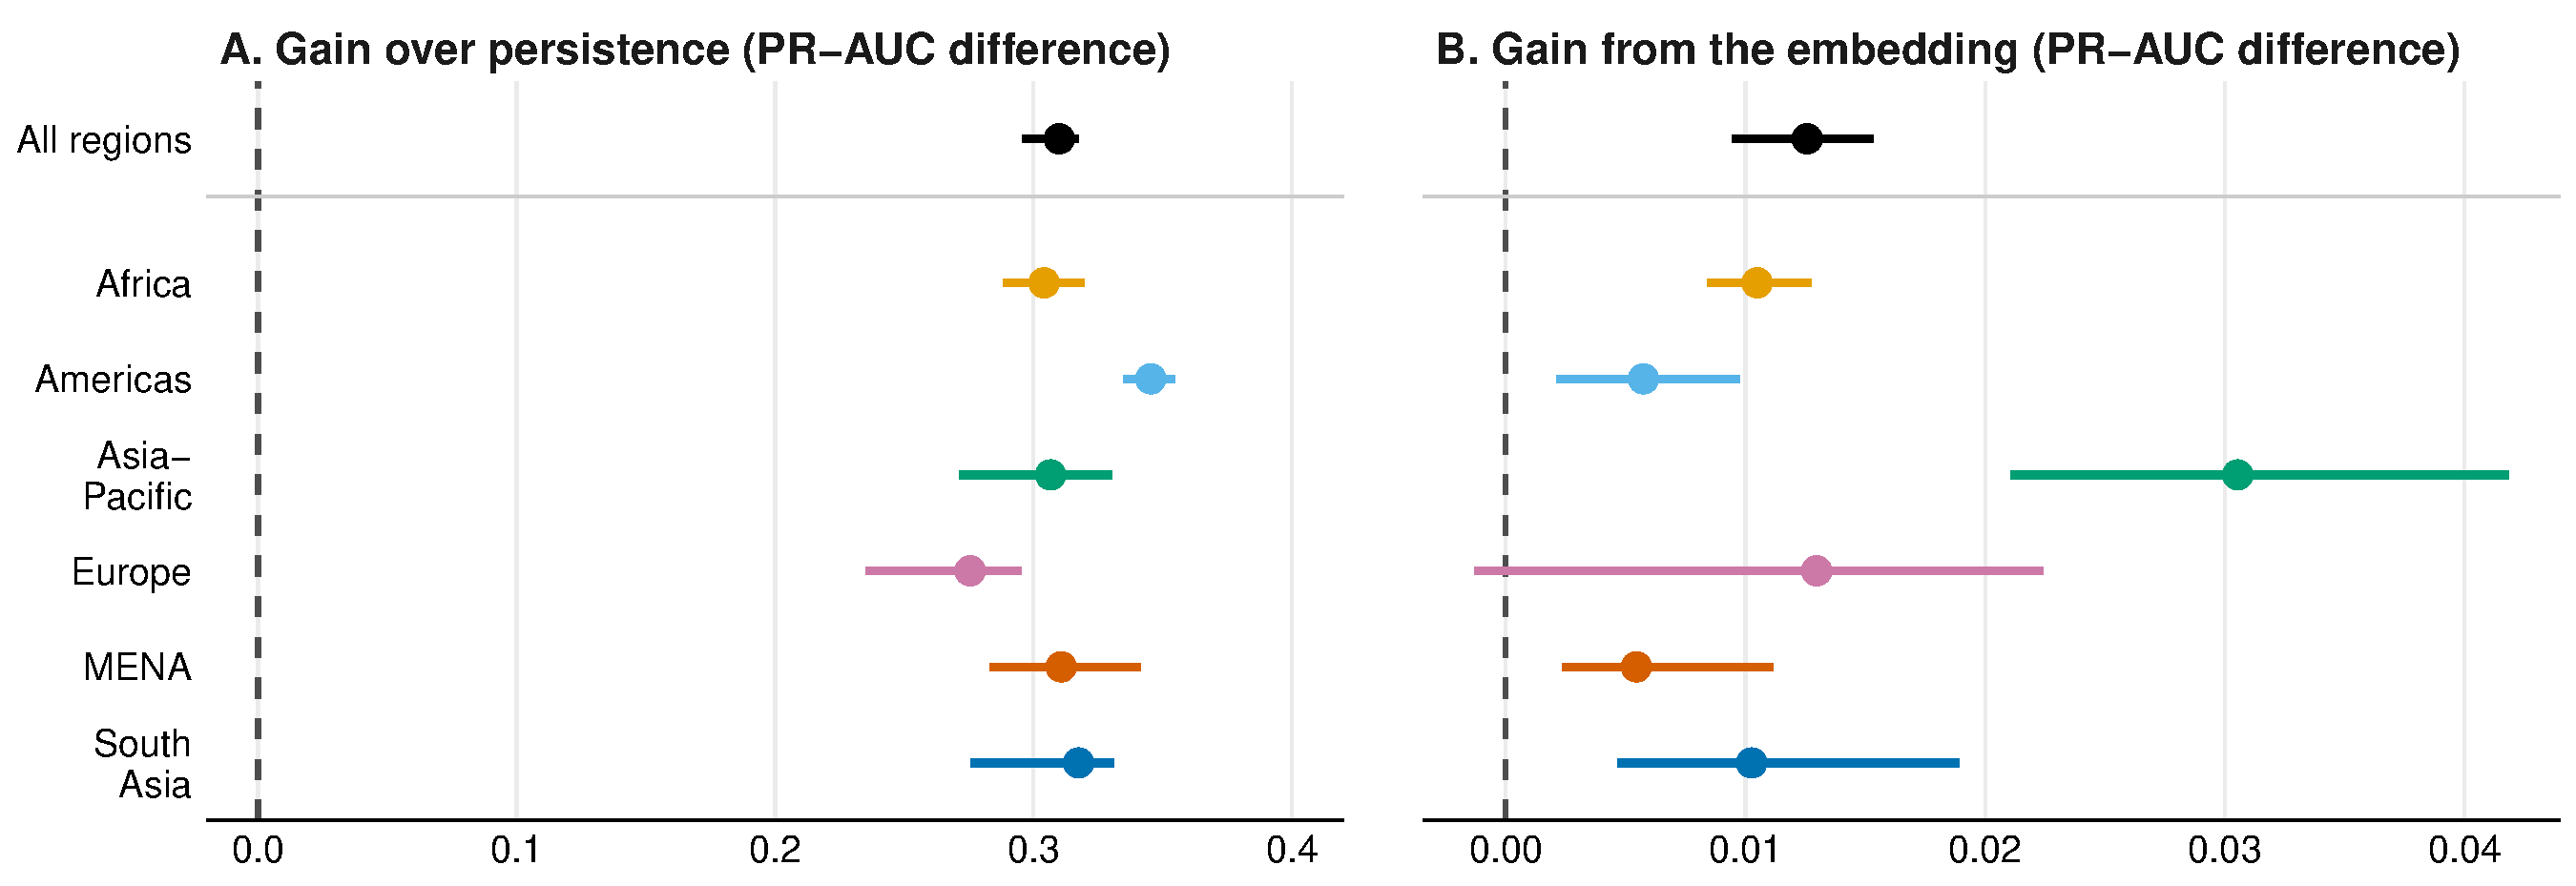
\includegraphics[width=\textwidth]{figures/fig_loro_gains.pdf}
\caption{Gain in PR-AUC over the persistence model (A) and over the base model without the embedding (B), by held-out region. Points show estimates and bars show 95\% bootstrap intervals.}
\label{fig:loro_gains}
\end{figure}


% Against the base model, the forecaster with the frozen embedding identifies 197 more violent cell-months in Africa, 184 more in the Americas, 151 more in Asia-Pacific, 60 more in Europe, 18 more in MENA, and 99 more in South Asia. 





\subsection{Fine-Tuning With Minimal Local Data}
\label{sec:finetune}
Figure~\ref{fig:finetune_gains} displays the fine-tuning results, with Panel A displaying the equal-weight mean across the six held-out regions and Panel B providing a breakdown by region.\footnote{See Appendix Section~\ref{app:finetune_table} for a full table of the results, including a variant that tunes only the top two layers.} With 0.25 percent of the training data, the fine-tuned encoder outperforms the network trained from scratch in five of the six regions, with gains ranging from +0.040 (South Asia) to +0.101 (Asia-Pacific), no change in Africa, and an equal-weight mean across the six regions of +0.053. This corresponds to 2,204 more violent cell-months identified at 0.25 percent compared with the network trained from scratch at the same number of alerts. The advantage reverses as more local data become available, which marks the boundary of where pretraining helps. 


\begin{figure}[t]
\centering
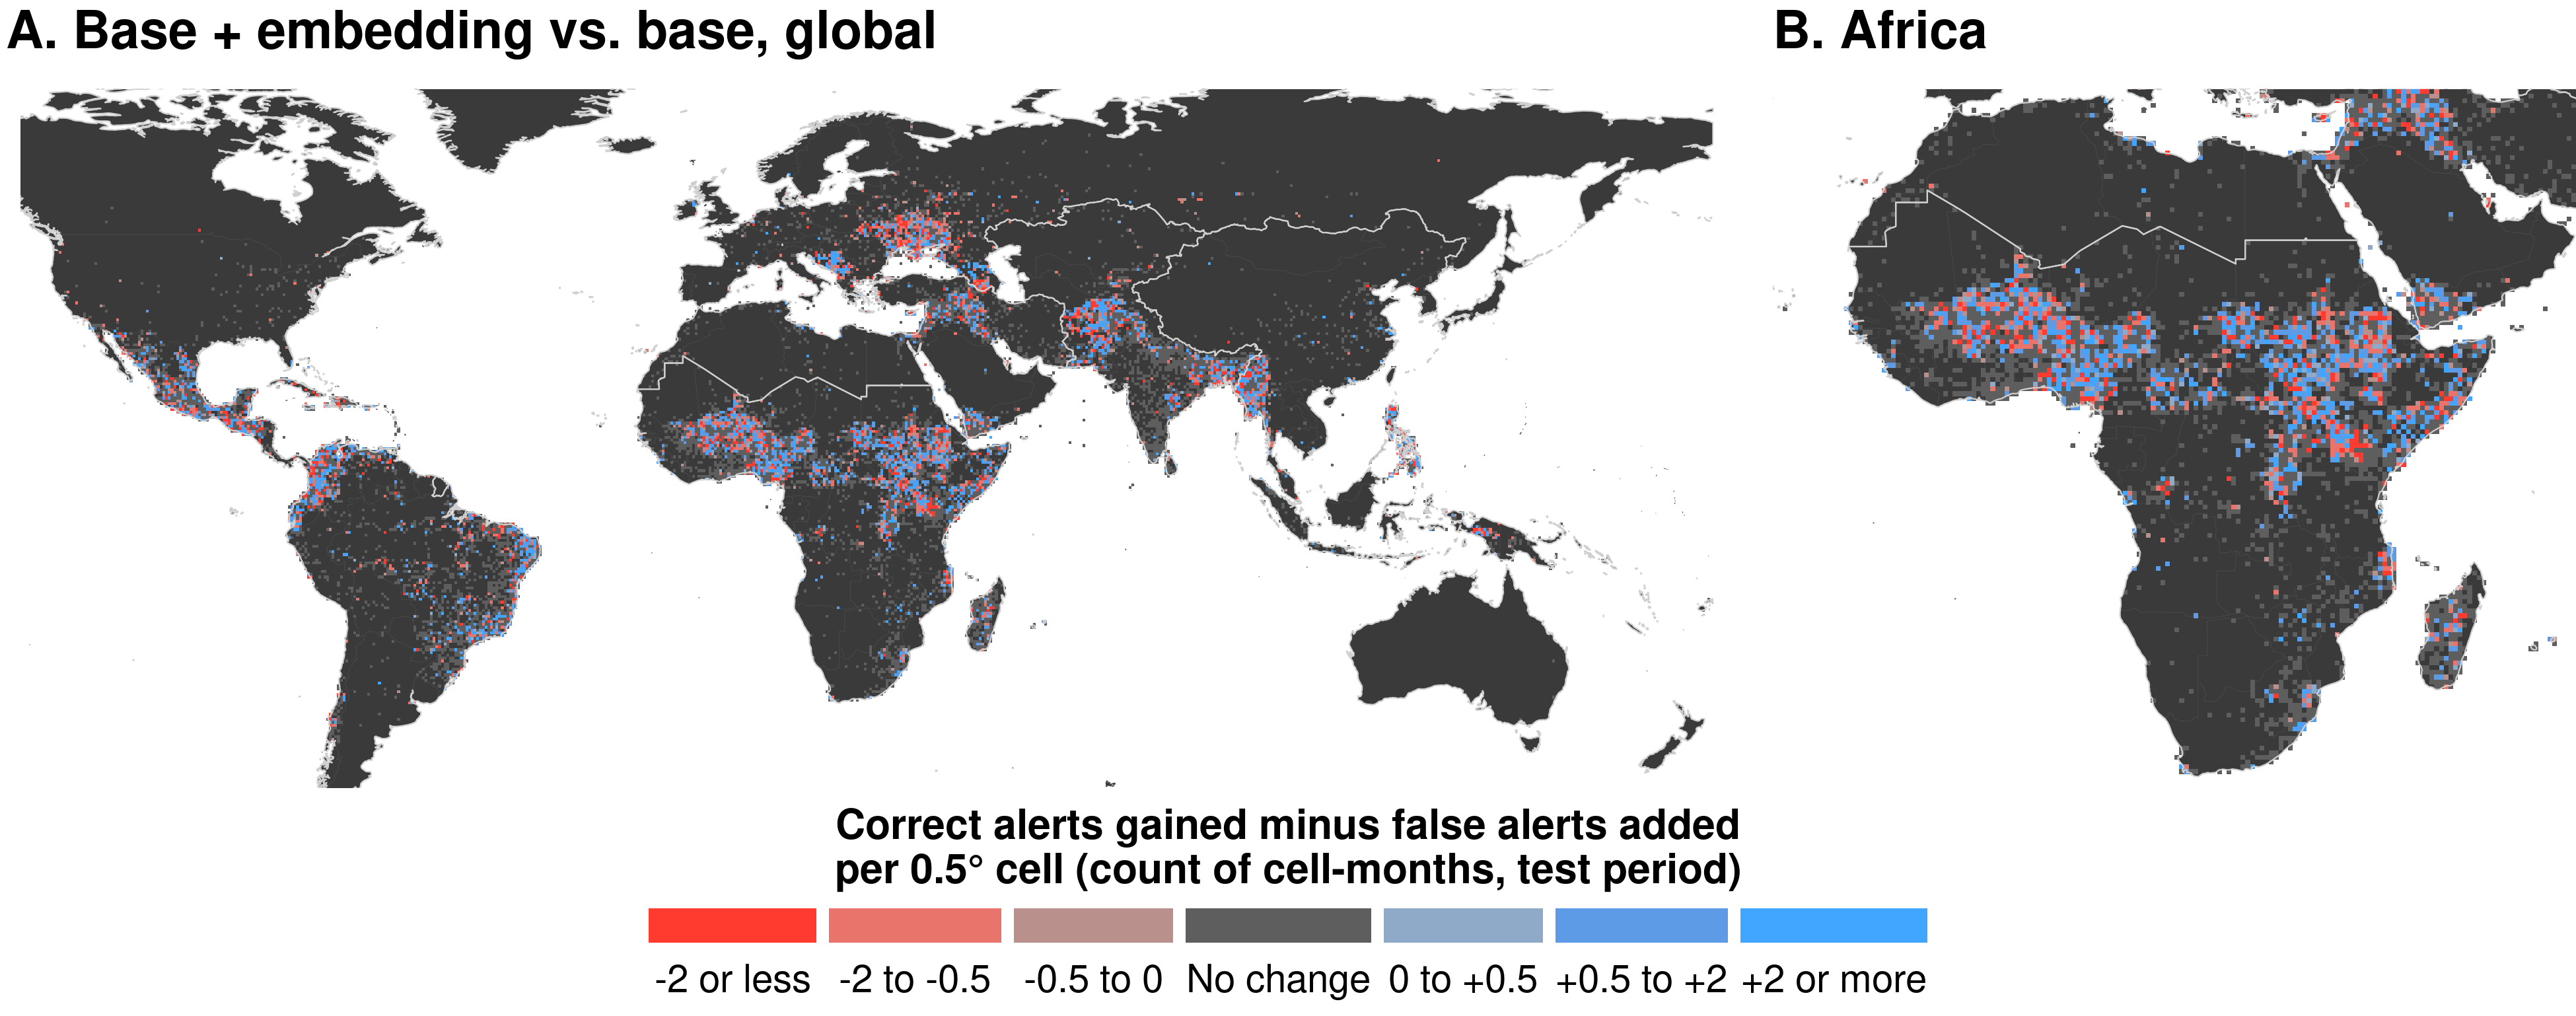
\includegraphics[width=\textwidth]{figures/fig_cell_alerts_maps_nested_M_fullsrc.png}
\caption{Each 0.5$^\circ$ cell shows true alarms gained minus false alarms added by the base plus embedding model relative to the base model, averaged over three encoder seeds, with the number of violent test cell-months as the alert count. Blue indicates gains; red indicates losses.}
\label{fig:cell_maps}
\end{figure}


At 0.5 percent, the fine-tuned encoder still improves forecasting overall, with a mean gain of +0.014 in PR-AUC, and the mean gain remains positive at 0.75 and 1 percent (+0.025 and +0.014, with intervals that exclude zero). Performance varies across regions. At 0.5 percent the gain excludes zero in the Americas, Asia-Pacific, and South Asia, and no region has a loss whose interval excludes zero. On average, the pretrained encoder does worse than the network trained from scratch at 2.5--10 percent. Pretraining is therefore most useful when labeled local data are very scarce, the setting transfer learning is meant for. 


\begin{figure}[t]
\centering
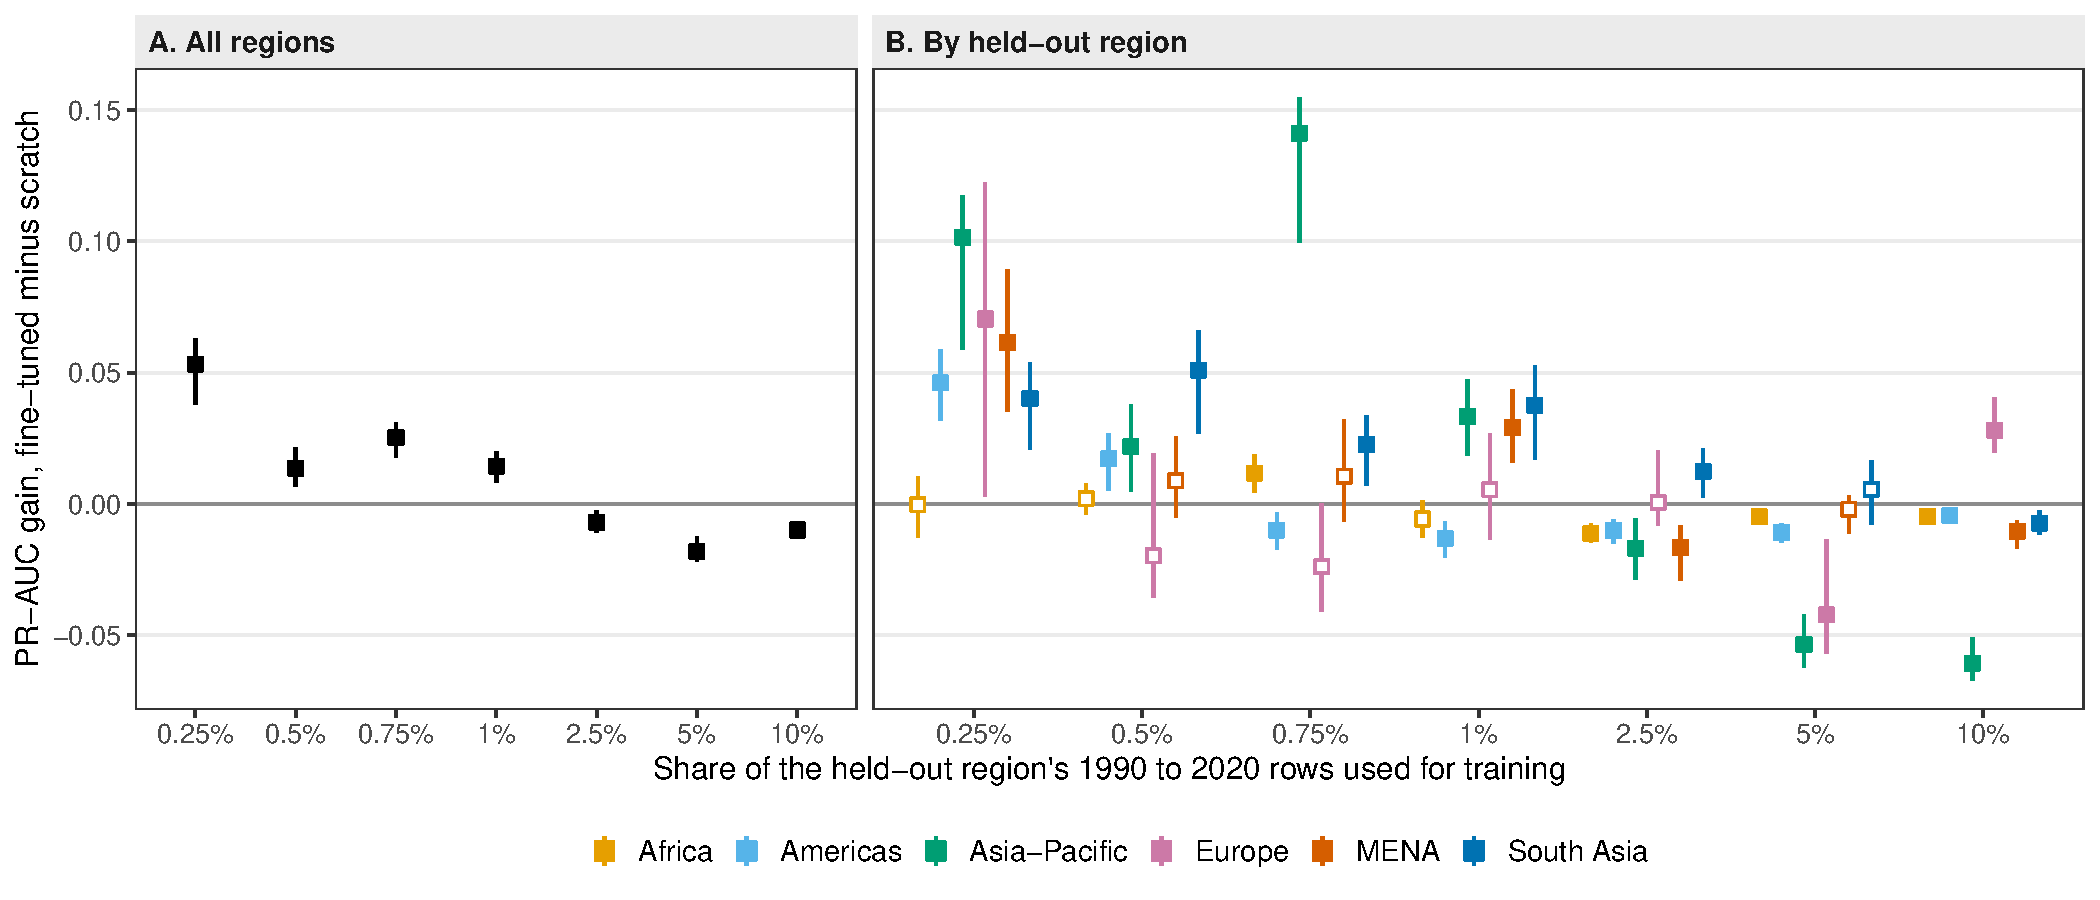
\includegraphics[width=\textwidth]{figures/fig_finetune_gains.pdf}
\caption{Gain from fine-tuning the pretrained encoder over the same network trained from scratch, by share of the held-out region's 1990--2020 training data (PR-AUC) with bars showing the 95\% bootstrap intervals. Panel A is the equal-weight mean across the six regions; Panel B is by region. Filled squares mark intervals that exclude zero.}
\label{fig:finetune_gains}
\end{figure}

\section{Transfer to New Domains}
\label{sec:brazil}
Across the three exercises, I find evidence that pretrained embeddings improve forecasting for conflict events in regions that were not part of the encoder's training data. Here, I assess whether the pretrained encoder can improve forecasting in new domains---homicides, suicides, traffic deaths, and drowning in Brazil, recorded in the Mortality Information System (SIM) \citep{sim_datasus}. This exploratory exercise tests whether the frozen conflict encoder improves forecasts of these four mortality outcomes.

For each outcome, I assign municipality-level deaths to PRIO-GRID cell-months using municipality centroids. Each death is recoded into the pretrained encoder's input fields, following how ACLED codes comparable events in Brazil.\footnote{See Appendix Section~\ref{app:vocab} for the mortality-record mapping, spatial aggregation, training periods, baseline features, and uncertainty procedure.}  I then compare a gradient-boosted forecaster with the frozen embedding, at 0.25 to 100 percent of the training data, against the same forecaster without the embedding. For each forecast origin $t$, I predict the count of deaths in month $t+1$ using predictors through $t-1$. Because these outcomes are counts rather than binary events, I compare Poisson deviance for origins from January 2022 to November 2024, corresponding to outcomes from February 2022 to December 2024.\footnote{Poisson deviance measures prediction error for counts, with lower values indicating better performance. Gains are relative deviance reductions, so positive values are better.}

Figure \ref{fig:placebo_gradient_ab_M} displays the results. In this comparison the embedding delivers a far smaller gain for drowning than for the other three outcomes at every training share, and the separation among outcomes is sharpest when local data are scarce. With 0.25 percent of Brazil's training data, the forecaster with the frozen embedding reduces Poisson deviance by 2.9 percent for homicides, 9.8 percent for suicides, and 5.0 percent for traffic deaths relative to the same forecaster without the embedding, and raises it by 1.0 percent for drowning. The homicide and drowning intervals both include zero.

\begin{figure}[t]
\centering
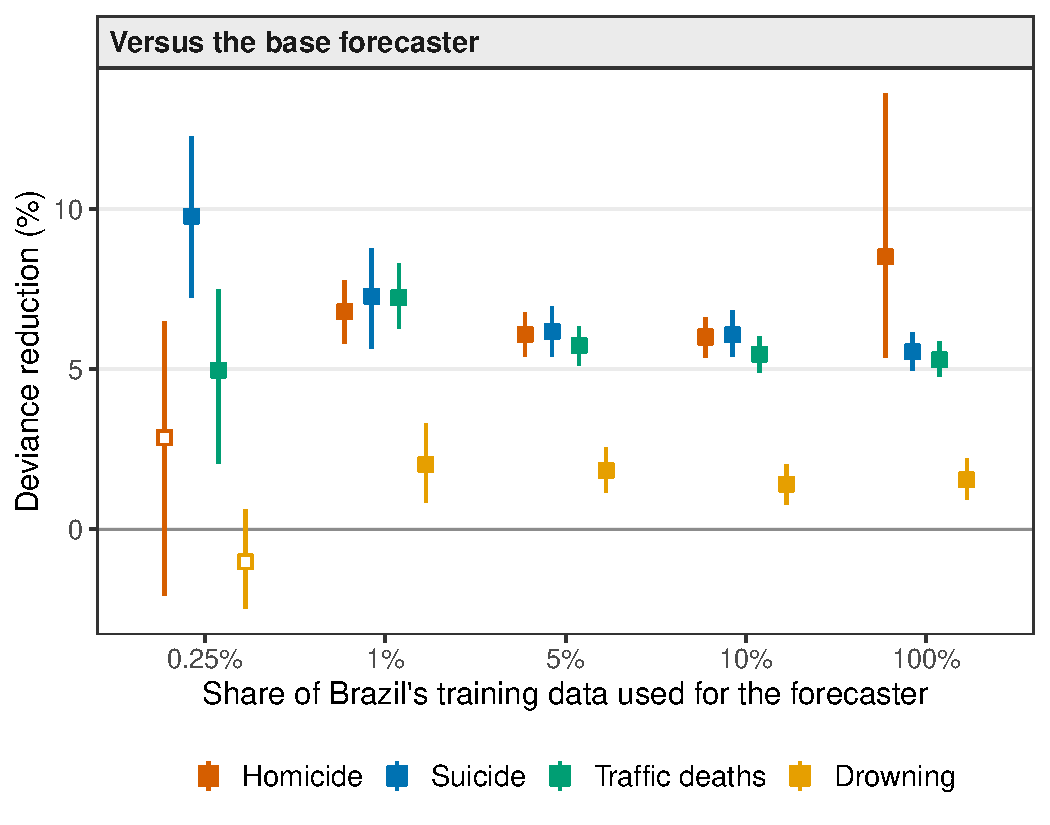
\includegraphics[width=\textwidth]{figures/fig_placebo_gradient_ab_M.pdf}
\caption{Relative reduction in Poisson deviance (\%) for the forecaster with the frozen embedding versus the same forecaster without it, by outcome and share of Brazil's training data. Positive values favor the embedding. Bars show 95\% bootstrap intervals from a two-way bootstrap that resamples grid cells and seed and draw pairs; filled squares mark intervals excluding zero.}
\label{fig:placebo_gradient_ab_M}
\end{figure}



%\section{Discussion}


\section{Discussion and Conclusion}
\label{sec:discussion}
In this article, I demonstrate how transformers can be used in transfer learning exercises outside of media data. This is, to my knowledge, the first political science study to pretrain a transformer encoder on structured event records and reuse it for transfer learning. Overall, the findings support geographic transfer learning, especially when local labels are scarce, and suggest potential for transfer across outcomes. Although I validate and test this approach in several ways, I wish to note three potential limitations.

First, I argue that transformers can be used for transfer learning across many unexplored domains in political science when high-dimensional data already exist. However, the main encoder is trained only on conflict data. In Appendix Section~\ref{app:domains}, I seek to address this issue with three alternative transfer learning exercises: (a) forecasting validated voter turnout in different regions using Cooperative Election Study (CES) data; (b) crime forecasting across cities in the United States; and (c) forecasting dengue spread across municipalities in Brazil. Each application pretrains its own domain-specific encoder and shows forecasting gains when local data are scarcest, with the gains persisting at larger shares for turnout and crime. %Specifically, with 0.25 percent of the training data, fine-tuning the pretrained encoder improves on the same network trained from scratch by +0.033 for CES turnout prediction, +0.085 for crime outcomes, and +0.059 for disease spread (Appendix Section~\ref{app:domains}). These correspond to 1,204, 3,799, and 121 more true alarms and 1,204, 3,799, and 121 fewer false alarms, respectively.


Second, I show that the inclusion of a pretrained encoder is useful for transfer learning in my forecasts. Notably, this does not rule out that the encoder architecture, rather than its pretraining, drives the observed gains. I address this in Appendix Section~\ref{app:random} by comparing the main results against a randomly initialized encoder in the same LORO design. A randomly initialized encoder with the same architecture recovers a portion of the embedding's gain, but the pretrained encoder scores higher in 14 of 18 region-seed runs (one-sided binomial test, $p = 0.015$), with a mean gain of +0.005 PR-AUC (95\% CI [0.002, 0.007]). 

%Third, for the main analyses, I pretrain the encoder with a contrastive objective. In turn, the observed results could be driven in part by that choice. I address this issue in Appendix Table~\ref{tab:ar_baseline} by pretraining the encoder with an autoregressive objective, which learns to predict the next event in a sequence, and evaluating it on 26 held-out countries. Adding this embedding improves the base model in all 15 combinations of feature set and seed (five feature sets; Appendix Sections~\ref{app:ar} and~\ref{app:pooled}).

Third, I assess transfer learning using a LORO test, in which a pretrained encoder is evaluated on future conflict data in places it has not seen. This design tests transfer to new regions rather than to new wars after long periods of peace, the early-warning setting that motivates the article. In the appendix, I use the 2022 Russia-Ukraine War as one such case and find that fine-tuning the encoder on 0.25 percent of Europe's training data improves forecasting in Ukraine over the test period relative to the network trained from scratch. Assessing transfer in short, recent conflict histories is a natural next step. 

%Fourth, in the article I show that transfer learning can be used for spatial politics through LORO and fine-tuning protocols. These findings suggest that spatial data in other parts of the world can be useful for forecasting conflict in new areas. However, these tests assess only whether any violent event occurs. In Appendix Section~\ref{app:ensemble}, I tune the pretrained encoders and test them on four outcomes in the held-out test data from January 2022 onward to assess how well the model forecasts civilian victimization, violence onset (violence in a cell with none the month before), overall violence, and fatal violence (25 or more deaths). The embedding clearly improves forecasts of civilian victimization and violence onset, matches the XGBoost forecaster on overall violence, and does not beat persistence for fatal violence.

The limitations notwithstanding, this article advances political scientists' understanding of transformers and transfer learning processes. Although I apply the pipeline to political violence, the implications of this article are wide-ranging in political science and social science scholarship broadly. Indeed, the present article suggests that scholars can achieve improvements in forecasting and labeling in political and social processes across a range of issues---e.g., predicting low-propensity voter behavior, disease spread, or crime. These issues, and many others, are plagued by small and sporadic amounts of data but are nevertheless consequential. Pretrained encoders and transfer learning in different domains can help us improve data labeling, prediction, and forecasting.

\section{References}
\bibliographystyle{apalike}
\bibliography{bibliography}


% ============================================================
% APPENDIX (unlimited length per USHMM/APSR norms -- put robustness detail here)
% ============================================================
\newpage
\appendix

\counterwithin{table}{section}
\counterwithin{figure}{section}

\renewcommand{\thetable}{\thesection\arabic{table}}
\renewcommand{\thefigure}{\thesection\arabic{figure}}
\ifdefined\theHtable \renewcommand{\theHtable}{A\arabic{table}}\fi   % keeps hyperref links unique
\ifdefined\theHfigure \renewcommand{\theHfigure}{A\arabic{figure}}\fi
% ADDED 2026-10-20 by Claude: appendix table of contents (titletoc; compile twice)
\startcontents[appendix]

\begin{singlespacing}

\section*{Appendix Contents}
\printcontents[appendix]{}{1}{\setcounter{tocdepth}{2}}

\end{singlespacing}

\newpage
\section{Supplementary Tables and Figures}
\label{app:supp}
This section contains supplementary details on the data pipeline, the encoder, and additional results. % EDIT: was "supplementary materials and tables on the data and figures"

\subsection{Data Pipeline}
Figure~\ref{fig:pipeline} groups the code by stage. Stage 01 builds the cell-month panel, the event records, and the baseline features. Stage 02 pretrains 18 leave-one-region-out encoders for each encoder size. Stages 03 and 04 run the frozen-embedding comparisons and the fine-tuning grids, and stages 05 and 06 compute the bootstrap intervals and alert counts. Stages 07 and 08 build and evaluate the Ukraine case, the Brazil mortality outcomes, and the turnout, crime, and dengue applications. Stage 09 writes every figure and table. A single driver (\texttt{pipeline/run.sh}) checks all inputs before submitting any job and then submits each stage through one job script (\texttt{pipeline/tasks.sbatch}). Raw ACLED data and the trained encoders are not distributed, in keeping with ACLED's terms of use.

% fig_pipeline.tex -- code pipeline of the consolidated replication package (pipeline/run.sh stages 00-09).
% Updated 2026-11-05 to the consolidated layout on branch consolidate-p1 (58-file manifest). Script names match the manifest.
% If the stage-01 merge (build_panel.py) is committed, replace the stage-01 script names with build_panel.py <step>.
% Requires tikz (already loaded in main.tex). Usage: % fig_pipeline.tex -- code pipeline of the consolidated replication package (pipeline/run.sh stages 00-09).
% Updated 2026-11-05 to the consolidated layout on branch consolidate-p1 (58-file manifest). Script names match the manifest.
% If the stage-01 merge (build_panel.py) is committed, replace the stage-01 script names with build_panel.py <step>.
% Requires tikz (already loaded in main.tex). Usage: % fig_pipeline.tex -- code pipeline of the consolidated replication package (pipeline/run.sh stages 00-09).
% Updated 2026-11-05 to the consolidated layout on branch consolidate-p1 (58-file manifest). Script names match the manifest.
% If the stage-01 merge (build_panel.py) is committed, replace the stage-01 script names with build_panel.py <step>.
% Requires tikz (already loaded in main.tex). Usage: \input{figures/fig_pipeline.tex}
\usetikzlibrary{positioning, arrows.meta, calc}
\begin{figure}[!htbp]
\centering
\resizebox{\textwidth}{!}{%
\begin{tikzpicture}[
font=\sffamily\small,
>={Stealth[length=2.3mm]},
sc/.style={draw=black!65, rounded corners=2pt, fill=#1, align=center, inner sep=4pt,
text width=5.4cm, minimum height=1.3cm,
execute at begin node={\hyphenpenalty=10000\exhyphenpenalty=10000}},
sc/.default=white,
src/.style={draw=black!65, fill=black!6, align=center, inner sep=4pt, text width=4.9cm, minimum height=1.0cm},
lane/.style={font=\sffamily\bfseries\small, text=black!55, rotate=90, anchor=south, align=center},
arr/.style={->, thick, draw=black!65},
ln/.style={draw=black!15, thick}
]
\definecolor{cB}{HTML}{DCE9F5}
\definecolor{cF}{HTML}{E8F1E4}
\definecolor{cP}{HTML}{EFE3F3}
\definecolor{cE}{HTML}{F7DADA}
\definecolor{cU}{HTML}{FBEFD9}
\definecolor{cO}{HTML}{F6E6CF}
\providecommand{\scr}[1]{{\ttfamily\footnotesize\bfseries #1}}
\def\xa{0}\def\xb{5.6}\def\xc{11.2}\def\xd{16.8}\def\xab{2.8}

% Sources
\node[src] (acled) at (\xa,0) {\textbf{ACLED events}};
\node[src] (ucdp) at (\xb,0) {\textbf{UCDP GED events}};
\node[src] (prio) at (\xc,0) {\textbf{PRIO-GRID covariates}};
\node[src] (oth) at (\xd,0) {\textbf{Other domains}\\ Brazil SIM deaths, CES, crime, dengue};

% Stage 01: panel and inputs
\node[sc=cB, text width=10.5cm] (ing) at (\xab,-2.0)
{\scr{build\_panel.py} steps acled, ucdp, merge\\
harmonize both sources to one event schema (settings in \scr{build\_panel.py})};
\node[sc=cB] (pst) at (\xc,-2.0) {\scr{build\_panel.py} step prio\\ standardize covariates};
\node[sc=cB] (dom) at (\xd,-2.0) {\scr{prep\_sim.py}, \scr{brazil\_panel.py}, \scr{prep\_ces.py}, \scr{crime\_ingest.py}, \scr{dengue\_ingest.py}\\ domain panels (run in stages 07--08)};
\node[sc=cB, text width=10.5cm] (grd) at (\xab,-4.0)
{\scr{build\_panel.py} steps grid, aggregate\\ cell-month panel and outcome};
\node[sc=cF] (seq) at (\xa,-6.2) {\scr{build\_panel.py} steps sequences, super, \scr{build\_seen\_tokens\_fullsrc.py}\\ event records for each cell-month};
\node[sc=cF] (fea) at (\xb,-6.2) {\scr{build\_panel.py} steps baseline, pgm\\ baseline features and targets};
\draw[arr] (acled) -- (acled |- ing.north);
\draw[arr] (ucdp) -- (ucdp |- ing.north);
\draw[arr] (prio) -- (pst);
\draw[arr] (oth) -- (dom);
\draw[arr] (ing) -- (grd);
\draw[arr] (grd.south -| seq.north) -- (seq.north);
\draw[arr] (grd.south -| fea.north) -- (fea.north);

% Stage 02: pretraining
\node[sc=cP, text width=10.5cm] (pre) at (\xab,-8.4)
{\scr{train\_repr\_obj.py}\\ 18 leave-one-region-out encoders per size (S, M, L), seeds 123, 456, 789};
\draw[arr] (seq) -- (seq |- pre.north);
\draw[thick, draw=black!65] (pst.south) -- (\xc,-7.45);
\draw[arr] (\xc,-7.45) -| ($(pre.north east)+(-0.4,0)$);

% Stages 03, 04, 07, 08: evaluation
\node[sc=cE] (e1) at (\xa,-11.0) {\scr{transfer\_eval\_region\_fullpreds.py}, \scr{vocab\_remap.py}\\ persistence, base, base plus embedding, random encoder};
\node[sc=cE] (e2) at (\xb,-11.0) {\scr{share\_grid\_fullsrc.py}\\ nested and fine-tuning grids, 7 shares $\times$ 5 draws $\times$ 3 seeds};
\node[sc=cE] (e3) at (\xc,-11.0) {\scr{country\_slice\_fullsrc.py}, \scr{country\_window\_fullsrc.py}\\ Ukraine};
\node[sc=cE] (e4) at (\xd,-11.0) {\scr{xd\_grid\_brazil\_v6.py} (Brazil); \scr{pretrain\_domain.py}, \scr{share\_grid\_domain.py}, \scr{pretrain\_ces.py}, \scr{share\_grid\_ces.py} (turnout, crime, dengue)};
\draw[arr] ($(pre.south)+(-3.4,0)$) -- ($(e1.north)+(-0.6,0)$);
\draw[arr] ($(pre.south)+(1.6,0)$) -- ($(e2.north)+(-1.2,0)$);
\draw[arr] (pre.east) -| (e3.north);
\draw[arr] (\xc,-8.4) -- (15.6,-8.4) -- ($(e4.north)+(-1.2,0)$);
\draw[arr] ($(dom.south)+(1.2,0)$) -- ($(e4.north)+(1.2,0)$);
\draw[thick, draw=black!65] (fea.east) -- (8.7,-6.2) -- (8.7,-9.95) -- (1.2,-9.95);
\draw[arr] (1.2,-9.95) -- (1.2,-9.95 |- e1.north);
\draw[arr] (6.8,-9.95) -- (6.8,-9.95 |- e2.north);

% Stages 05, 06, 07, 08: intervals, alerts, maps
\node[sc=cU] (b1) at (\xa,-13.8) {\scr{bootstrap\_ci\_fullsrc.py}, \scr{alert\_counts\_fullsrc.py}, \scr{cell\_alerts\_agg\_fullsrc.py}, \scr{persistence\_month\_t\_fullsrc.py}};
\node[sc=cU] (b2) at (\xb,-13.8) {\scr{bootstrap\_ft\_fullsrc.py},\\ {\ttfamily\scriptsize\bfseries alert\_counts\_finetune\_fullsrc\_full.py}};
\node[sc=cU] (b3) at (\xc,-13.8) {\scr{export\_ukraine\_map\_fullsrc.py}\\ Ukraine maps};
\node[sc=cU] (b4) at (\xd,-13.8) {\scr{xd\_boot.py}, \scr{xd\_placebo\_boot\_v3M.py}, \scr{domain\_tp\_fp\_f0025.py}};
\draw[arr] (e1) -- (b1); \draw[arr] (e2) -- (b2); \draw[arr] (e3) -- (b3); \draw[arr] (e4) -- (b4);

% Stage 09: outputs
\node[sc=cO, text width=21.2cm] (out) at (8.4,-16.4)
{\scr{figures.R}, \scr{make\_tables.py}\\ every generated figure and table in the article and appendix};
\draw[arr] (b1) -- (b1 |- out.north); \draw[arr] (b2) -- (b2 |- out.north);
\draw[arr] (b3) -- (b3 |- out.north); \draw[arr] (b4) -- (b4 |- out.north);

% Lane labels and guides
\foreach \y/\t in {0/Sources, -4.1/Stage 01, -8.4/Stage 02, -11.0/{Stages 03, 04,\\ 07, 08}, -13.8/{Stages 05--08}, -16.4/Stage 09} {
\node[lane] at (-2.85,\y) {\t};
}
\foreach \y in {-0.8, -7.3, -9.6, -12.4, -15.2} {
\draw[ln] (-3.6,\y) -- (19.4,\y);
}
\end{tikzpicture}%
}
\caption{\textbf{Code pipeline.} The driver \texttt{pipeline/run.sh} checks all inputs (stage 00) and then submits stages 01 to 09 as Slurm jobs through one job script, \texttt{pipeline/tasks.sbatch}. Each box names the scripts that perform a step. Every conflict model trains on months through December 2020, and all reported conflict forecasts are for January 2022 onward.}
\label{fig:pipeline}
\end{figure}

\usetikzlibrary{positioning, arrows.meta, calc}
\begin{figure}[!htbp]
\centering
\resizebox{\textwidth}{!}{%
\begin{tikzpicture}[
font=\sffamily\small,
>={Stealth[length=2.3mm]},
sc/.style={draw=black!65, rounded corners=2pt, fill=#1, align=center, inner sep=4pt,
text width=5.4cm, minimum height=1.3cm,
execute at begin node={\hyphenpenalty=10000\exhyphenpenalty=10000}},
sc/.default=white,
src/.style={draw=black!65, fill=black!6, align=center, inner sep=4pt, text width=4.9cm, minimum height=1.0cm},
lane/.style={font=\sffamily\bfseries\small, text=black!55, rotate=90, anchor=south, align=center},
arr/.style={->, thick, draw=black!65},
ln/.style={draw=black!15, thick}
]
\definecolor{cB}{HTML}{DCE9F5}
\definecolor{cF}{HTML}{E8F1E4}
\definecolor{cP}{HTML}{EFE3F3}
\definecolor{cE}{HTML}{F7DADA}
\definecolor{cU}{HTML}{FBEFD9}
\definecolor{cO}{HTML}{F6E6CF}
\providecommand{\scr}[1]{{\ttfamily\footnotesize\bfseries #1}}
\def\xa{0}\def\xb{5.6}\def\xc{11.2}\def\xd{16.8}\def\xab{2.8}

% Sources
\node[src] (acled) at (\xa,0) {\textbf{ACLED events}};
\node[src] (ucdp) at (\xb,0) {\textbf{UCDP GED events}};
\node[src] (prio) at (\xc,0) {\textbf{PRIO-GRID covariates}};
\node[src] (oth) at (\xd,0) {\textbf{Other domains}\\ Brazil SIM deaths, CES, crime, dengue};

% Stage 01: panel and inputs
\node[sc=cB, text width=10.5cm] (ing) at (\xab,-2.0)
{\scr{build\_panel.py} steps acled, ucdp, merge\\
harmonize both sources to one event schema (settings in \scr{build\_panel.py})};
\node[sc=cB] (pst) at (\xc,-2.0) {\scr{build\_panel.py} step prio\\ standardize covariates};
\node[sc=cB] (dom) at (\xd,-2.0) {\scr{prep\_sim.py}, \scr{brazil\_panel.py}, \scr{prep\_ces.py}, \scr{crime\_ingest.py}, \scr{dengue\_ingest.py}\\ domain panels (run in stages 07--08)};
\node[sc=cB, text width=10.5cm] (grd) at (\xab,-4.0)
{\scr{build\_panel.py} steps grid, aggregate\\ cell-month panel and outcome};
\node[sc=cF] (seq) at (\xa,-6.2) {\scr{build\_panel.py} steps sequences, super, \scr{build\_seen\_tokens\_fullsrc.py}\\ event records for each cell-month};
\node[sc=cF] (fea) at (\xb,-6.2) {\scr{build\_panel.py} steps baseline, pgm\\ baseline features and targets};
\draw[arr] (acled) -- (acled |- ing.north);
\draw[arr] (ucdp) -- (ucdp |- ing.north);
\draw[arr] (prio) -- (pst);
\draw[arr] (oth) -- (dom);
\draw[arr] (ing) -- (grd);
\draw[arr] (grd.south -| seq.north) -- (seq.north);
\draw[arr] (grd.south -| fea.north) -- (fea.north);

% Stage 02: pretraining
\node[sc=cP, text width=10.5cm] (pre) at (\xab,-8.4)
{\scr{train\_repr\_obj.py}\\ 18 leave-one-region-out encoders per size (S, M, L), seeds 123, 456, 789};
\draw[arr] (seq) -- (seq |- pre.north);
\draw[thick, draw=black!65] (pst.south) -- (\xc,-7.45);
\draw[arr] (\xc,-7.45) -| ($(pre.north east)+(-0.4,0)$);

% Stages 03, 04, 07, 08: evaluation
\node[sc=cE] (e1) at (\xa,-11.0) {\scr{transfer\_eval\_region\_fullpreds.py}, \scr{vocab\_remap.py}\\ persistence, base, base plus embedding, random encoder};
\node[sc=cE] (e2) at (\xb,-11.0) {\scr{share\_grid\_fullsrc.py}\\ nested and fine-tuning grids, 7 shares $\times$ 5 draws $\times$ 3 seeds};
\node[sc=cE] (e3) at (\xc,-11.0) {\scr{country\_slice\_fullsrc.py}, \scr{country\_window\_fullsrc.py}\\ Ukraine};
\node[sc=cE] (e4) at (\xd,-11.0) {\scr{xd\_grid\_brazil\_v6.py} (Brazil); \scr{pretrain\_domain.py}, \scr{share\_grid\_domain.py}, \scr{pretrain\_ces.py}, \scr{share\_grid\_ces.py} (turnout, crime, dengue)};
\draw[arr] ($(pre.south)+(-3.4,0)$) -- ($(e1.north)+(-0.6,0)$);
\draw[arr] ($(pre.south)+(1.6,0)$) -- ($(e2.north)+(-1.2,0)$);
\draw[arr] (pre.east) -| (e3.north);
\draw[arr] (\xc,-8.4) -- (15.6,-8.4) -- ($(e4.north)+(-1.2,0)$);
\draw[arr] ($(dom.south)+(1.2,0)$) -- ($(e4.north)+(1.2,0)$);
\draw[thick, draw=black!65] (fea.east) -- (8.7,-6.2) -- (8.7,-9.95) -- (1.2,-9.95);
\draw[arr] (1.2,-9.95) -- (1.2,-9.95 |- e1.north);
\draw[arr] (6.8,-9.95) -- (6.8,-9.95 |- e2.north);

% Stages 05, 06, 07, 08: intervals, alerts, maps
\node[sc=cU] (b1) at (\xa,-13.8) {\scr{bootstrap\_ci\_fullsrc.py}, \scr{alert\_counts\_fullsrc.py}, \scr{cell\_alerts\_agg\_fullsrc.py}, \scr{persistence\_month\_t\_fullsrc.py}};
\node[sc=cU] (b2) at (\xb,-13.8) {\scr{bootstrap\_ft\_fullsrc.py},\\ {\ttfamily\scriptsize\bfseries alert\_counts\_finetune\_fullsrc\_full.py}};
\node[sc=cU] (b3) at (\xc,-13.8) {\scr{export\_ukraine\_map\_fullsrc.py}\\ Ukraine maps};
\node[sc=cU] (b4) at (\xd,-13.8) {\scr{xd\_boot.py}, \scr{xd\_placebo\_boot\_v3M.py}, \scr{domain\_tp\_fp\_f0025.py}};
\draw[arr] (e1) -- (b1); \draw[arr] (e2) -- (b2); \draw[arr] (e3) -- (b3); \draw[arr] (e4) -- (b4);

% Stage 09: outputs
\node[sc=cO, text width=21.2cm] (out) at (8.4,-16.4)
{\scr{figures.R}, \scr{make\_tables.py}\\ every generated figure and table in the article and appendix};
\draw[arr] (b1) -- (b1 |- out.north); \draw[arr] (b2) -- (b2 |- out.north);
\draw[arr] (b3) -- (b3 |- out.north); \draw[arr] (b4) -- (b4 |- out.north);

% Lane labels and guides
\foreach \y/\t in {0/Sources, -4.1/Stage 01, -8.4/Stage 02, -11.0/{Stages 03, 04,\\ 07, 08}, -13.8/{Stages 05--08}, -16.4/Stage 09} {
\node[lane] at (-2.85,\y) {\t};
}
\foreach \y in {-0.8, -7.3, -9.6, -12.4, -15.2} {
\draw[ln] (-3.6,\y) -- (19.4,\y);
}
\end{tikzpicture}%
}
\caption{\textbf{Code pipeline.} The driver \texttt{pipeline/run.sh} checks all inputs (stage 00) and then submits stages 01 to 09 as Slurm jobs through one job script, \texttt{pipeline/tasks.sbatch}. Each box names the scripts that perform a step. Every conflict model trains on months through December 2020, and all reported conflict forecasts are for January 2022 onward.}
\label{fig:pipeline}
\end{figure}

\usetikzlibrary{positioning, arrows.meta, calc}
\begin{figure}[!htbp]
\centering
\resizebox{\textwidth}{!}{%
\begin{tikzpicture}[
font=\sffamily\small,
>={Stealth[length=2.3mm]},
sc/.style={draw=black!65, rounded corners=2pt, fill=#1, align=center, inner sep=4pt,
text width=5.4cm, minimum height=1.3cm,
execute at begin node={\hyphenpenalty=10000\exhyphenpenalty=10000}},
sc/.default=white,
src/.style={draw=black!65, fill=black!6, align=center, inner sep=4pt, text width=4.9cm, minimum height=1.0cm},
lane/.style={font=\sffamily\bfseries\small, text=black!55, rotate=90, anchor=south, align=center},
arr/.style={->, thick, draw=black!65},
ln/.style={draw=black!15, thick}
]
\definecolor{cB}{HTML}{DCE9F5}
\definecolor{cF}{HTML}{E8F1E4}
\definecolor{cP}{HTML}{EFE3F3}
\definecolor{cE}{HTML}{F7DADA}
\definecolor{cU}{HTML}{FBEFD9}
\definecolor{cO}{HTML}{F6E6CF}
\providecommand{\scr}[1]{{\ttfamily\footnotesize\bfseries #1}}
\def\xa{0}\def\xb{5.6}\def\xc{11.2}\def\xd{16.8}\def\xab{2.8}

% Sources
\node[src] (acled) at (\xa,0) {\textbf{ACLED events}};
\node[src] (ucdp) at (\xb,0) {\textbf{UCDP GED events}};
\node[src] (prio) at (\xc,0) {\textbf{PRIO-GRID covariates}};
\node[src] (oth) at (\xd,0) {\textbf{Other domains}\\ Brazil SIM deaths, CES, crime, dengue};

% Stage 01: panel and inputs
\node[sc=cB, text width=10.5cm] (ing) at (\xab,-2.0)
{\scr{build\_panel.py} steps acled, ucdp, merge\\
harmonize both sources to one event schema (settings in \scr{build\_panel.py})};
\node[sc=cB] (pst) at (\xc,-2.0) {\scr{build\_panel.py} step prio\\ standardize covariates};
\node[sc=cB] (dom) at (\xd,-2.0) {\scr{prep\_sim.py}, \scr{brazil\_panel.py}, \scr{prep\_ces.py}, \scr{crime\_ingest.py}, \scr{dengue\_ingest.py}\\ domain panels (run in stages 07--08)};
\node[sc=cB, text width=10.5cm] (grd) at (\xab,-4.0)
{\scr{build\_panel.py} steps grid, aggregate\\ cell-month panel and outcome};
\node[sc=cF] (seq) at (\xa,-6.2) {\scr{build\_panel.py} steps sequences, super, \scr{build\_seen\_tokens\_fullsrc.py}\\ event records for each cell-month};
\node[sc=cF] (fea) at (\xb,-6.2) {\scr{build\_panel.py} steps baseline, pgm\\ baseline features and targets};
\draw[arr] (acled) -- (acled |- ing.north);
\draw[arr] (ucdp) -- (ucdp |- ing.north);
\draw[arr] (prio) -- (pst);
\draw[arr] (oth) -- (dom);
\draw[arr] (ing) -- (grd);
\draw[arr] (grd.south -| seq.north) -- (seq.north);
\draw[arr] (grd.south -| fea.north) -- (fea.north);

% Stage 02: pretraining
\node[sc=cP, text width=10.5cm] (pre) at (\xab,-8.4)
{\scr{train\_repr\_obj.py}\\ 18 leave-one-region-out encoders per size (S, M, L), seeds 123, 456, 789};
\draw[arr] (seq) -- (seq |- pre.north);
\draw[thick, draw=black!65] (pst.south) -- (\xc,-7.45);
\draw[arr] (\xc,-7.45) -| ($(pre.north east)+(-0.4,0)$);

% Stages 03, 04, 07, 08: evaluation
\node[sc=cE] (e1) at (\xa,-11.0) {\scr{transfer\_eval\_region\_fullpreds.py}, \scr{vocab\_remap.py}\\ persistence, base, base plus embedding, random encoder};
\node[sc=cE] (e2) at (\xb,-11.0) {\scr{share\_grid\_fullsrc.py}\\ nested and fine-tuning grids, 7 shares $\times$ 5 draws $\times$ 3 seeds};
\node[sc=cE] (e3) at (\xc,-11.0) {\scr{country\_slice\_fullsrc.py}, \scr{country\_window\_fullsrc.py}\\ Ukraine};
\node[sc=cE] (e4) at (\xd,-11.0) {\scr{xd\_grid\_brazil\_v6.py} (Brazil); \scr{pretrain\_domain.py}, \scr{share\_grid\_domain.py}, \scr{pretrain\_ces.py}, \scr{share\_grid\_ces.py} (turnout, crime, dengue)};
\draw[arr] ($(pre.south)+(-3.4,0)$) -- ($(e1.north)+(-0.6,0)$);
\draw[arr] ($(pre.south)+(1.6,0)$) -- ($(e2.north)+(-1.2,0)$);
\draw[arr] (pre.east) -| (e3.north);
\draw[arr] (\xc,-8.4) -- (15.6,-8.4) -- ($(e4.north)+(-1.2,0)$);
\draw[arr] ($(dom.south)+(1.2,0)$) -- ($(e4.north)+(1.2,0)$);
\draw[thick, draw=black!65] (fea.east) -- (8.7,-6.2) -- (8.7,-9.95) -- (1.2,-9.95);
\draw[arr] (1.2,-9.95) -- (1.2,-9.95 |- e1.north);
\draw[arr] (6.8,-9.95) -- (6.8,-9.95 |- e2.north);

% Stages 05, 06, 07, 08: intervals, alerts, maps
\node[sc=cU] (b1) at (\xa,-13.8) {\scr{bootstrap\_ci\_fullsrc.py}, \scr{alert\_counts\_fullsrc.py}, \scr{cell\_alerts\_agg\_fullsrc.py}, \scr{persistence\_month\_t\_fullsrc.py}};
\node[sc=cU] (b2) at (\xb,-13.8) {\scr{bootstrap\_ft\_fullsrc.py},\\ {\ttfamily\scriptsize\bfseries alert\_counts\_finetune\_fullsrc\_full.py}};
\node[sc=cU] (b3) at (\xc,-13.8) {\scr{export\_ukraine\_map\_fullsrc.py}\\ Ukraine maps};
\node[sc=cU] (b4) at (\xd,-13.8) {\scr{xd\_boot.py}, \scr{xd\_placebo\_boot\_v3M.py}, \scr{domain\_tp\_fp\_f0025.py}};
\draw[arr] (e1) -- (b1); \draw[arr] (e2) -- (b2); \draw[arr] (e3) -- (b3); \draw[arr] (e4) -- (b4);

% Stage 09: outputs
\node[sc=cO, text width=21.2cm] (out) at (8.4,-16.4)
{\scr{figures.R}, \scr{make\_tables.py}\\ every generated figure and table in the article and appendix};
\draw[arr] (b1) -- (b1 |- out.north); \draw[arr] (b2) -- (b2 |- out.north);
\draw[arr] (b3) -- (b3 |- out.north); \draw[arr] (b4) -- (b4 |- out.north);

% Lane labels and guides
\foreach \y/\t in {0/Sources, -4.1/Stage 01, -8.4/Stage 02, -11.0/{Stages 03, 04,\\ 07, 08}, -13.8/{Stages 05--08}, -16.4/Stage 09} {
\node[lane] at (-2.85,\y) {\t};
}
\foreach \y in {-0.8, -7.3, -9.6, -12.4, -15.2} {
\draw[ln] (-3.6,\y) -- (19.4,\y);
}
\end{tikzpicture}%
}
\caption{\textbf{Code pipeline.} The driver \texttt{pipeline/run.sh} checks all inputs (stage 00) and then submits stages 01 to 09 as Slurm jobs through one job script, \texttt{pipeline/tasks.sbatch}. Each box names the scripts that perform a step. Every conflict model trains on months through December 2020, and all reported conflict forecasts are for January 2022 onward.}
\label{fig:pipeline}
\end{figure}


\subsection{Encoder Implementation Details}
\label{app:encoder_details}
In each vocabulary, zero and one are reserved. Zero is used for padding. Because units contain different numbers of records, empty slots are filled with zeros so that every unit has the same length, and padding slots receive no attention weight. % EDIT: merged "the model ignores these slots" with "padding slots also receive no attention weight", which said the same thing
In every field except the month offset, one is used for unknown values, meaning any value not in the vocabulary, either because it did not appear in the training data or because it falls outside the most frequent values kept for that field.

Whether to add positional encodings depends on the data. They are needed when the order of records carries meaning, as with words in a sentence, and can be omitted when records form an unordered set, with any timing information entered as a field. Here the records in a cell-month form an unordered set, so no positional encodings are used and timing enters through the month-offset field.

Following \citet{chen2020simclr}, the contrastive loss is computed on a small projection of the two embeddings rather than on the embeddings themselves. The positive pair is two augmented views of the same cell-month, and every other cell-month in the batch is treated as a negative, including cell-months with similar event histories. Grouping similar histories together is therefore a property the representation may learn, not something the loss enforces directly. Pretraining runs for at most 30 epochs and stops when the contrastive loss on the 2021 validation data has not improved for 15 consecutive epochs. The XGBoost settings are maximum depth 6, learning rate 0.1, subsample 0.8, column subsample 0.8, and 200 rounds.

\subsection{Frozen Embedding Comparison}
In the main text, I compare the frozen embedding against a persistence model and an XGBoost forecaster with and without the embedding. Table~\ref{tab:nested_embbase} displays point estimates for the same comparisons under the pooled evaluation, in which test cell-months are drawn across all years in five folds. The table reports the base plus embedding model against persistence and the base model with and without the embedding. The gains in the pooled evaluation are smaller than in the temporal test.

% UPDATED 2026-10-26 (Claude) to the M full-source encoders: eval_region_M_contrastive_e_fullsrc_loro_* (A_pooled_f0-4 means, incidence). Persistence (month t) column unchanged: it does not depend on the encoder (base and month t-1 persistence reproduce the old values exactly).
\begin{table}[!htbp]
\centering\footnotesize\setlength{\tabcolsep}{4pt}
\caption{Held-out regions, pooled five-fold test: persistence, base model and base model with the embedding (PR-AUC)}
\label{tab:nested_embbase}
\begin{tabular}{lcccccc}
\hline
 & \multicolumn{3}{c}{PR-AUC} & Base + emb. & Base + emb. & Runs \\
Held-out region & Persistence & Base & Base + emb. & $-$ persistence & $-$ base & gain $>0$ \\
\hline
Africa & 0.237 & 0.544 & 0.555 & $+0.317$ & $+0.010$ & 3/3 \\
Americas & 0.278 & 0.642 & 0.650 & $+0.372$ & $+0.009$ & 3/3 \\
Asia-Pacific & 0.261 & 0.609 & 0.617 & $+0.356$ & $+0.008$ & 3/3 \\
Europe & 0.326 & 0.662 & 0.664 & $+0.338$ & $+0.002$ & 3/3 \\
MENA & 0.426 & 0.764 & 0.770 & $+0.344$ & $+0.005$ & 3/3 \\
South Asia & 0.306 & 0.649 & 0.658 & $+0.352$ & $+0.009$ & 3/3 \\
\hline
All regions & 0.306 & 0.645 & 0.652 & $+0.347$ & $+0.007$ & 18/18 \\
\hline
\end{tabular}
\begin{minipage}{0.98\textwidth}\footnotesize\vspace{0.5ex}
Notes. Means over three encoder seeds (123, 456, 789). Target is any violent event in the 0.5$^\circ$ cell in month $t+1$; all models use information through month $t$. Persistence is the presence of violence in month $t$. Base is gradient boosting on hand-built and PRIO-GRID features; Base + emb. adds the frozen encoder embedding. Runs gain $>0$ counts region-seed runs in which Base + emb. beats Base. Pooled scores average five folds drawn over cell-months. Persistence measured in month $t-1$ averages 0.285.
\end{minipage}
\end{table}


% CUT 2026-11-08 (needs a multi-day GPU rerun; Jared): \subsection{Interregion Transfer}
% FLAG: the transfer matrix and network come from the old single-source L encoders (seed 123, scratch at a fixed learning rate of 1e-4). Their scripts are not in the replication pipeline. Cut or rerun before submission.
% CUT 2026-11-08 (needs a multi-day GPU rerun; Jared): In the main text, I use held-out regions for the pretrained encoder and a test region. Here, I display how well encoders pretrained on a single source region transfer to each target region. Table~\ref{tab:transfer_matrix} displays the results.

% CUT 2026-11-08 (needs a multi-day GPU rerun; Jared): Each source encoder is fine-tuned on 1 and 5 percent of the target region's training data and compared with the same network trained from scratch on the same rows. The diagonal cells display an encoder pretrained on only the target region, and the last row is the LORO encoder.

% CUT 2026-11-08 (needs a multi-day GPU rerun; Jared): At 1 percent, most of the pairs gain, and the LORO encoder gains in five of six regions. At 5 percent, those results mostly disappear or reverse, matching the boundary results in the main text.\footnote{The gains in Europe are from an unstable scratch baseline with a PR-AUC of 0.18.}

% CUT 2026-11-08 (needs a multi-day GPU rerun; Jared): \input{tables/table_transfer_matrix.tex}

% CUT 2026-11-08 (needs a multi-day GPU rerun; Jared): Figure~\ref{fig:transfer_network} breaks it down as a weighted network. Arrows run from the source to the target region, with the width indicating the size of the gain or loss. Blue arrows indicate a gain and orange arrows indicate a loss. Through this, we can see that the regions generally provide gains for Europe at 1 percent; every source region improves forecasts for MENA and the Americas at 1 percent, and the Americas encoder improves forecasts in every target region; and at 5 percent, every source region still improves forecasts for South Asia, while every source region lowers them for Asia-Pacific.

% CUT 2026-11-08 (needs a multi-day GPU rerun; Jared): \input{figures/fig_transfer_network.tex} % EDIT: moved up from the end of the section
\section{Pretrained Versus Random Encoder}
\label{app:random}
In the main text, I assess whether a pretrained encoder can be used for transfer learning. Here, I assess how much of the transfer effect is due to the encoder's architecture versus its pretraining. To do so, I compare the main results against an XGBoost model that uses an encoder with the same architecture and random initialization for the LORO nested analyses.

Table~\ref{tab:random_temporal} displays the results of the nested models against a randomly initialized encoder. The pretrained encoder improves on the base model by +0.013, while the random encoder improves on it by +0.008. The pretrained encoder beats the random encoder in 14 of 18 region-seed runs. This suggests that pretraining accounts for +0.005 PR-AUC (95\% block bootstrap interval [+0.002, +0.007]). For the pooled estimates, the gap is +0.001 and positive in 15 of 18 runs (see Table~\ref{tab:random_pooled} for point estimates and Figure~\ref{fig:random} for a comparison of both tests).

% UPDATED 2026-10-26 (Claude) to M full-source: eval_region_M_contrastive_e_fullsrc_loro_*_s{seed}.csv vs *_rand.csv (B_temporal, incidence).
\begin{table}[!htbp]
\centering\footnotesize\setlength{\tabcolsep}{5pt}
\caption{Political violence, temporal test: gain from a pretrained and a random encoder}
\label{tab:random_temporal}
\begin{tabular}{lccccc}
\hline
 & PR-AUC & \multicolumn{2}{c}{Gain over base} & Pretrained & Runs \\
Held-out region & Base & Pretrained encoder & Random encoder & $-$ random & difference $>0$ \\
\hline
Africa & 0.661 & $+0.010$ & $+0.008$ & $+0.003$ & 3/3 \\
Americas & 0.698 & $+0.006$ & $+0.004$ & $+0.001$ & 3/3 \\
Asia-Pacific & 0.716 & $+0.031$ & $+0.012$ & $+0.019$ & 3/3 \\
Europe & 0.672 & $+0.013$ & $+0.011$ & $+0.001$ & 2/3 \\
MENA & 0.820 & $+0.005$ & $+0.005$ & $+0.000$ & 1/3 \\
South Asia & 0.575 & $+0.010$ & $+0.008$ & $+0.002$ & 2/3 \\
\hline
All regions & 0.690 & $+0.013$ & $+0.008$ & $+0.005$ & 14/18 \\
\hline
\end{tabular}
\begin{minipage}{0.98\textwidth}\footnotesize\vspace{0.5ex}
Notes. Means over three encoder seeds. Gain over base is the PR-AUC of base + embedding minus base. The random encoder has the same architecture and random weights; the base model and test rows are identical across the two arms. Temporal test as in Figure~\ref{fig:loro_gains}.
\end{minipage}
\end{table}

% UPDATED 2026-10-26 (Claude) to M full-source: same files, A_pooled_f0-4 means.
\begin{table}[!htbp]
\centering\footnotesize\setlength{\tabcolsep}{5pt}
\caption{Political violence, pooled five-fold test: gain from a pretrained and a random encoder}
\label{tab:random_pooled}
\begin{tabular}{lccccc}
\hline
 & PR-AUC & \multicolumn{2}{c}{Gain over base} & Pretrained & Runs \\
Held-out region & Base & Pretrained encoder & Random encoder & $-$ random & difference $>0$ \\
\hline
Africa & 0.544 & $+0.010$ & $+0.009$ & $+0.002$ & 3/3 \\
Americas & 0.642 & $+0.009$ & $+0.006$ & $+0.003$ & 3/3 \\
Asia-Pacific & 0.609 & $+0.008$ & $+0.006$ & $+0.001$ & 3/3 \\
Europe & 0.662 & $+0.002$ & $+0.004$ & $-0.002$ & 0/3 \\
MENA & 0.764 & $+0.005$ & $+0.004$ & $+0.001$ & 3/3 \\
South Asia & 0.649 & $+0.009$ & $+0.008$ & $+0.002$ & 3/3 \\
\hline
All regions & 0.645 & $+0.007$ & $+0.006$ & $+0.001$ & 15/18 \\
\hline
\end{tabular}
\begin{minipage}{0.98\textwidth}\footnotesize\vspace{0.5ex}
Notes. Means over three encoder seeds. Gain over base is the PR-AUC of base + embedding minus base. The random encoder has the same architecture and random weights; the base model and test rows are identical across the two arms. Pooled scores average five folds.
\end{minipage}
\end{table}


\begin{figure}[t]
\centering
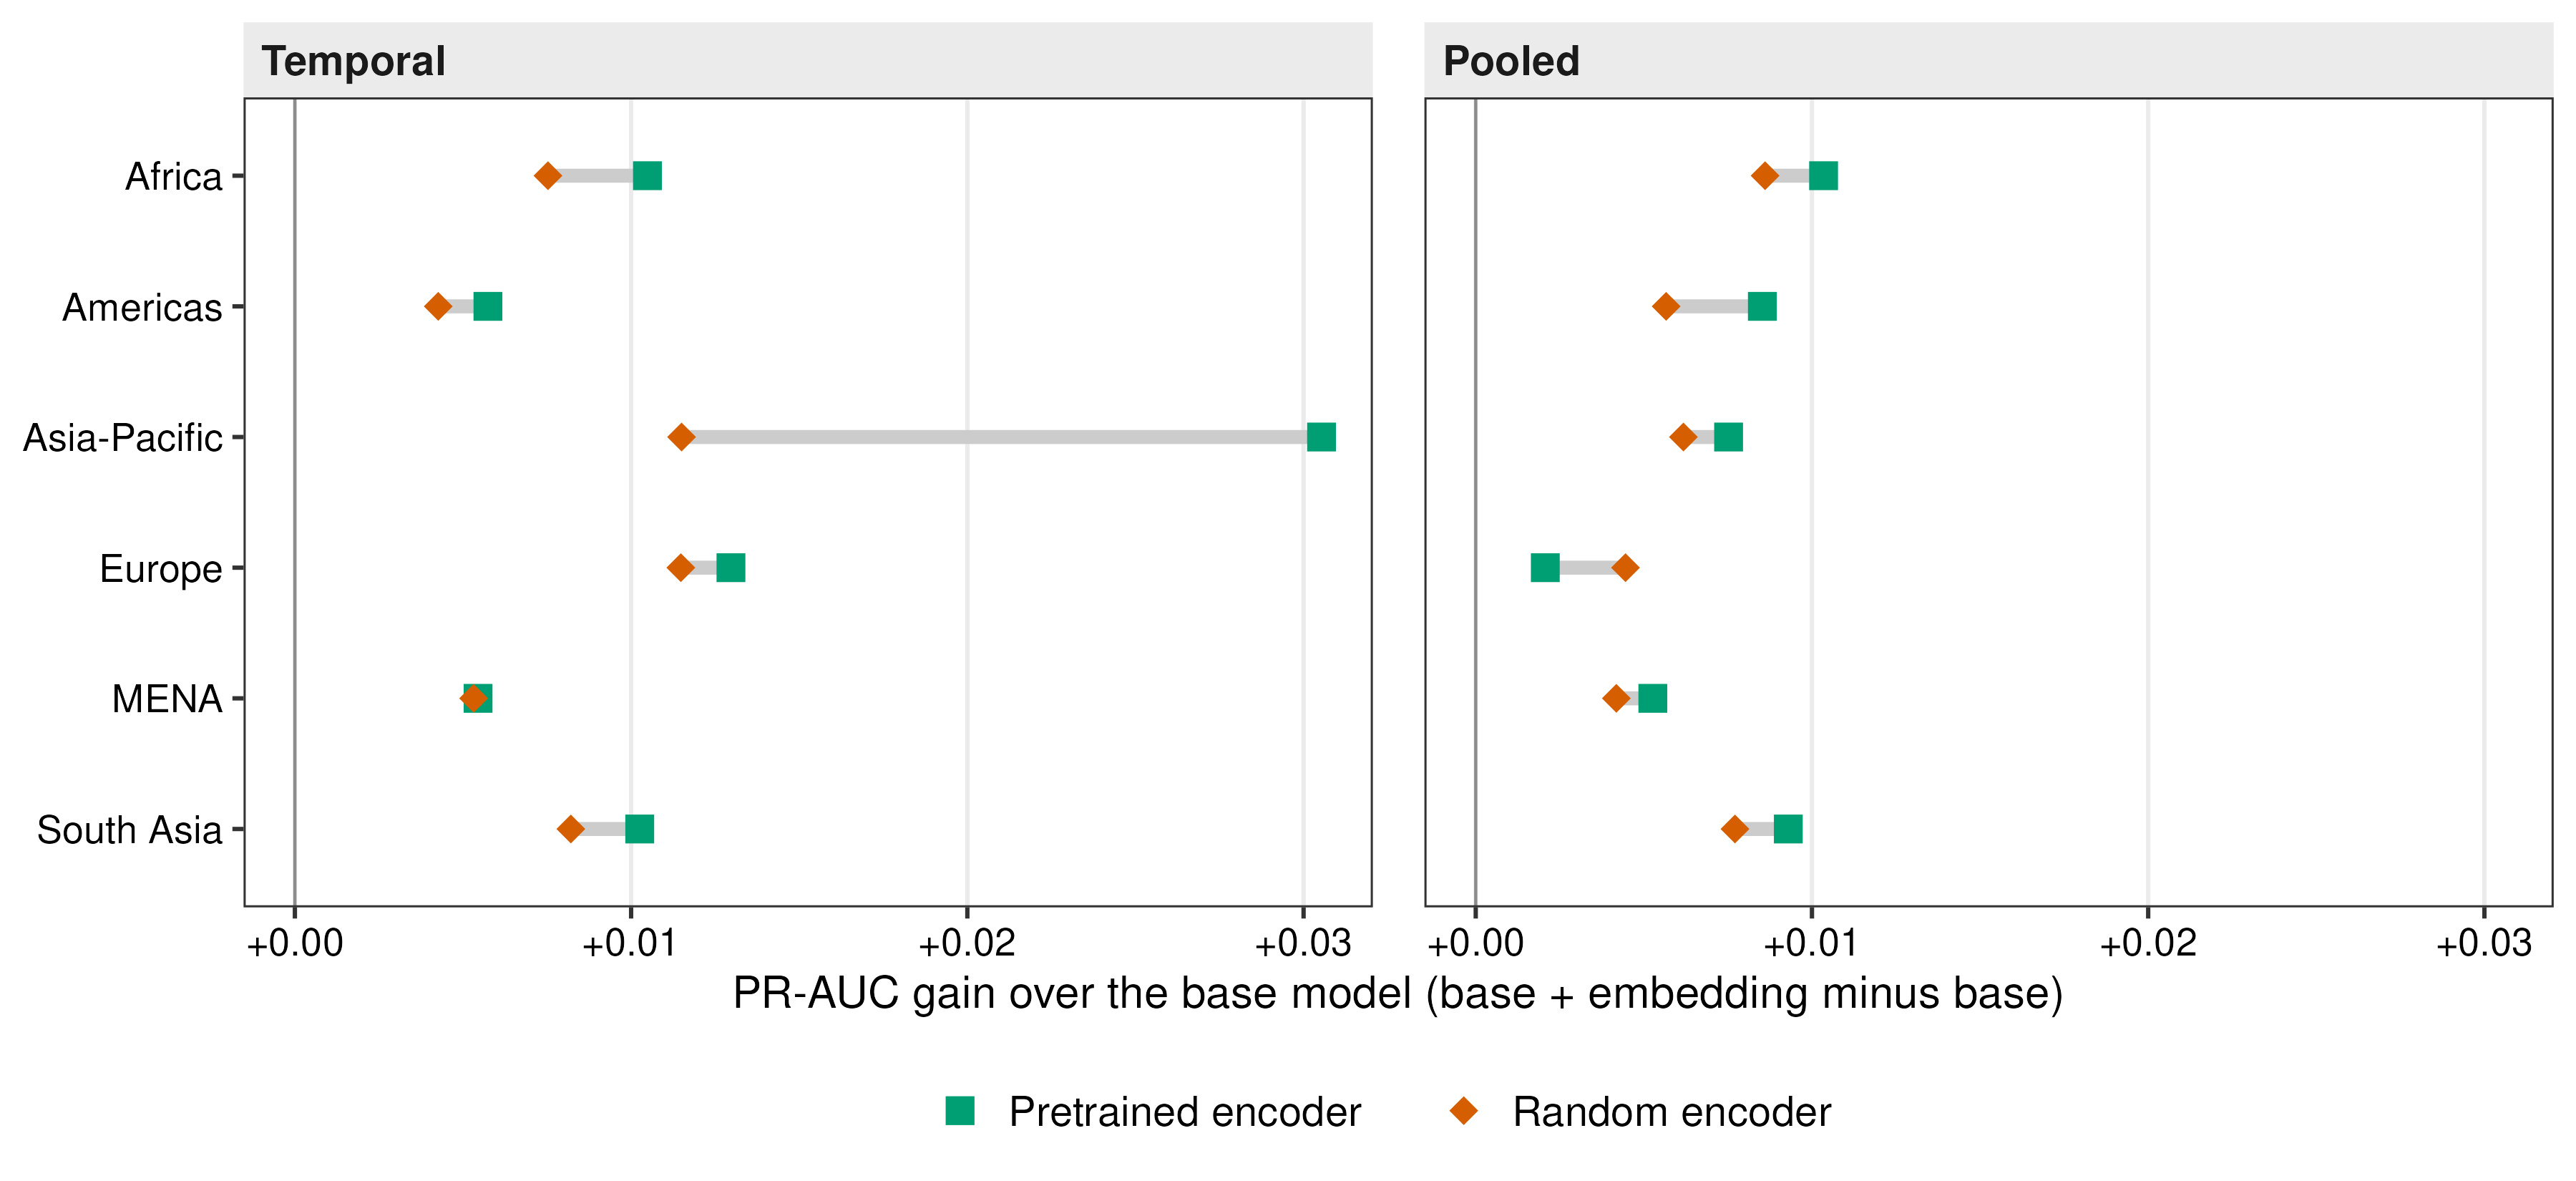
\includegraphics[width=\textwidth]{figures/fig_random_encoder.png}
\caption{Gain in PR-AUC over the base model from the pretrained encoder (squares) and from a random-weight encoder with the same architecture (diamonds), by held-out region, for the temporal test (left) and the pooled five-fold test (right). Points are means over three encoder seeds. The gap between the two markers is the gain from pretraining.}
\label{fig:random}
\end{figure}

% MOVED from the main text 2026-10-16
\section{Frozen Embedding With Minimal Local Data}
\label{app:shares}
Table~\ref{tab:pretrained_1pct} displays model performance when the held-out region's training data are limited to between 0.25 and 10 percent. I compare held-out region performance for a forecaster using the frozen embedding and features versus a features-alone forecaster; the encoder itself is never retrained. In five of six regions (Africa, the Americas, Asia-Pacific, MENA and South Asia), the frozen embeddings improve model performance at every share, with gains of +0.008 to +0.043. With 1 percent of the training data, the models with the frozen embeddings improve the PR-AUC in five regions, with gains of +0.013 to +0.035 in those regions. Averaged over all six regions, the gain at 1 percent is +0.008 [+0.004, +0.017], and the average gain is positive at every share from 0.25 to 10 percent (Figure~\ref{fig:boot_shares}). Europe is the exception. With very few violent training cell-months (15 at 0.25 percent and 59 at 1 percent), adding the embedding lowers performance at every share below 10 percent. In the five regions that gain at 1 percent, issuing the same number of alerts, the models with the frozen embeddings flag [alert count pending] more violent cell-months, and therefore raise as many fewer false alarms.

% UPDATED 2026-10-26 (Claude) to M full-source: outputs/share_grid_fullsrc/metrics_M_nested_{region}_s{seed}.csv, means over 3 seeds x 5 draws.
\begin{table}[!htbp]
\centering\footnotesize\setlength{\tabcolsep}{4pt}
\caption{Held-out regions with limited local data, temporal test: gain from adding the embedding to the base model (PR-AUC)}
\label{tab:pretrained_1pct}
\begin{tabular}{lccccccc}
\hline
 & \multicolumn{7}{c}{Share of the held-out region's training data} \\
Held-out region & 0.25\% & 0.5\% & 0.75\% & 1\% & 2.5\% & 5\% & 10\% \\
\hline
Africa & $+0.024$ & $+0.023$ & $+0.026$ & $+0.029$ & $+0.022$ & $+0.018$ & $+0.011$ \\
Americas & $+0.022$ & $+0.020$ & $+0.017$ & $+0.022$ & $+0.023$ & $+0.019$ & $+0.012$ \\
Asia-Pacific & $+0.037$ & $+0.017$ & $+0.026$ & $+0.013$ & $+0.024$ & $+0.035$ & $+0.017$ \\
Europe & $-0.077$ & $-0.034$ & $-0.036$ & $-0.065$ & $-0.029$ & $-0.010$ & $+0.010$ \\
MENA & $+0.009$ & $+0.016$ & $+0.012$ & $+0.015$ & $+0.018$ & $+0.015$ & $+0.008$ \\
South Asia & $+0.031$ & $+0.043$ & $+0.037$ & $+0.035$ & $+0.026$ & $+0.020$ & $+0.010$ \\
\hline
Mean & $+0.008$ & $+0.014$ & $+0.014$ & $+0.008$ & $+0.014$ & $+0.016$ & $+0.011$ \\
Regions $>0$ & 5/6 & 5/6 & 5/6 & 5/6 & 5/6 & 5/6 & 6/6 \\
\hline
\end{tabular}
\begin{minipage}{0.98\textwidth}\footnotesize\vspace{0.5ex}
Notes. Base + embedding minus base, both trained on the stated share of the held-out region's training months and scored on the full temporal test.
Means over three encoder seeds and five random draws of the training share. The encoder itself is never retrained.
Europe has very few violent training cell-months at small shares (15, 30, 44, 59, 148, 296 and 593 across the seven shares).
Fine-tuned pretrained versus scratch encoders: Appendix Table~\ref{tab:finetune_grid_full}.
\end{minipage}
\end{table}

\begin{figure}[!htbp]
\centering
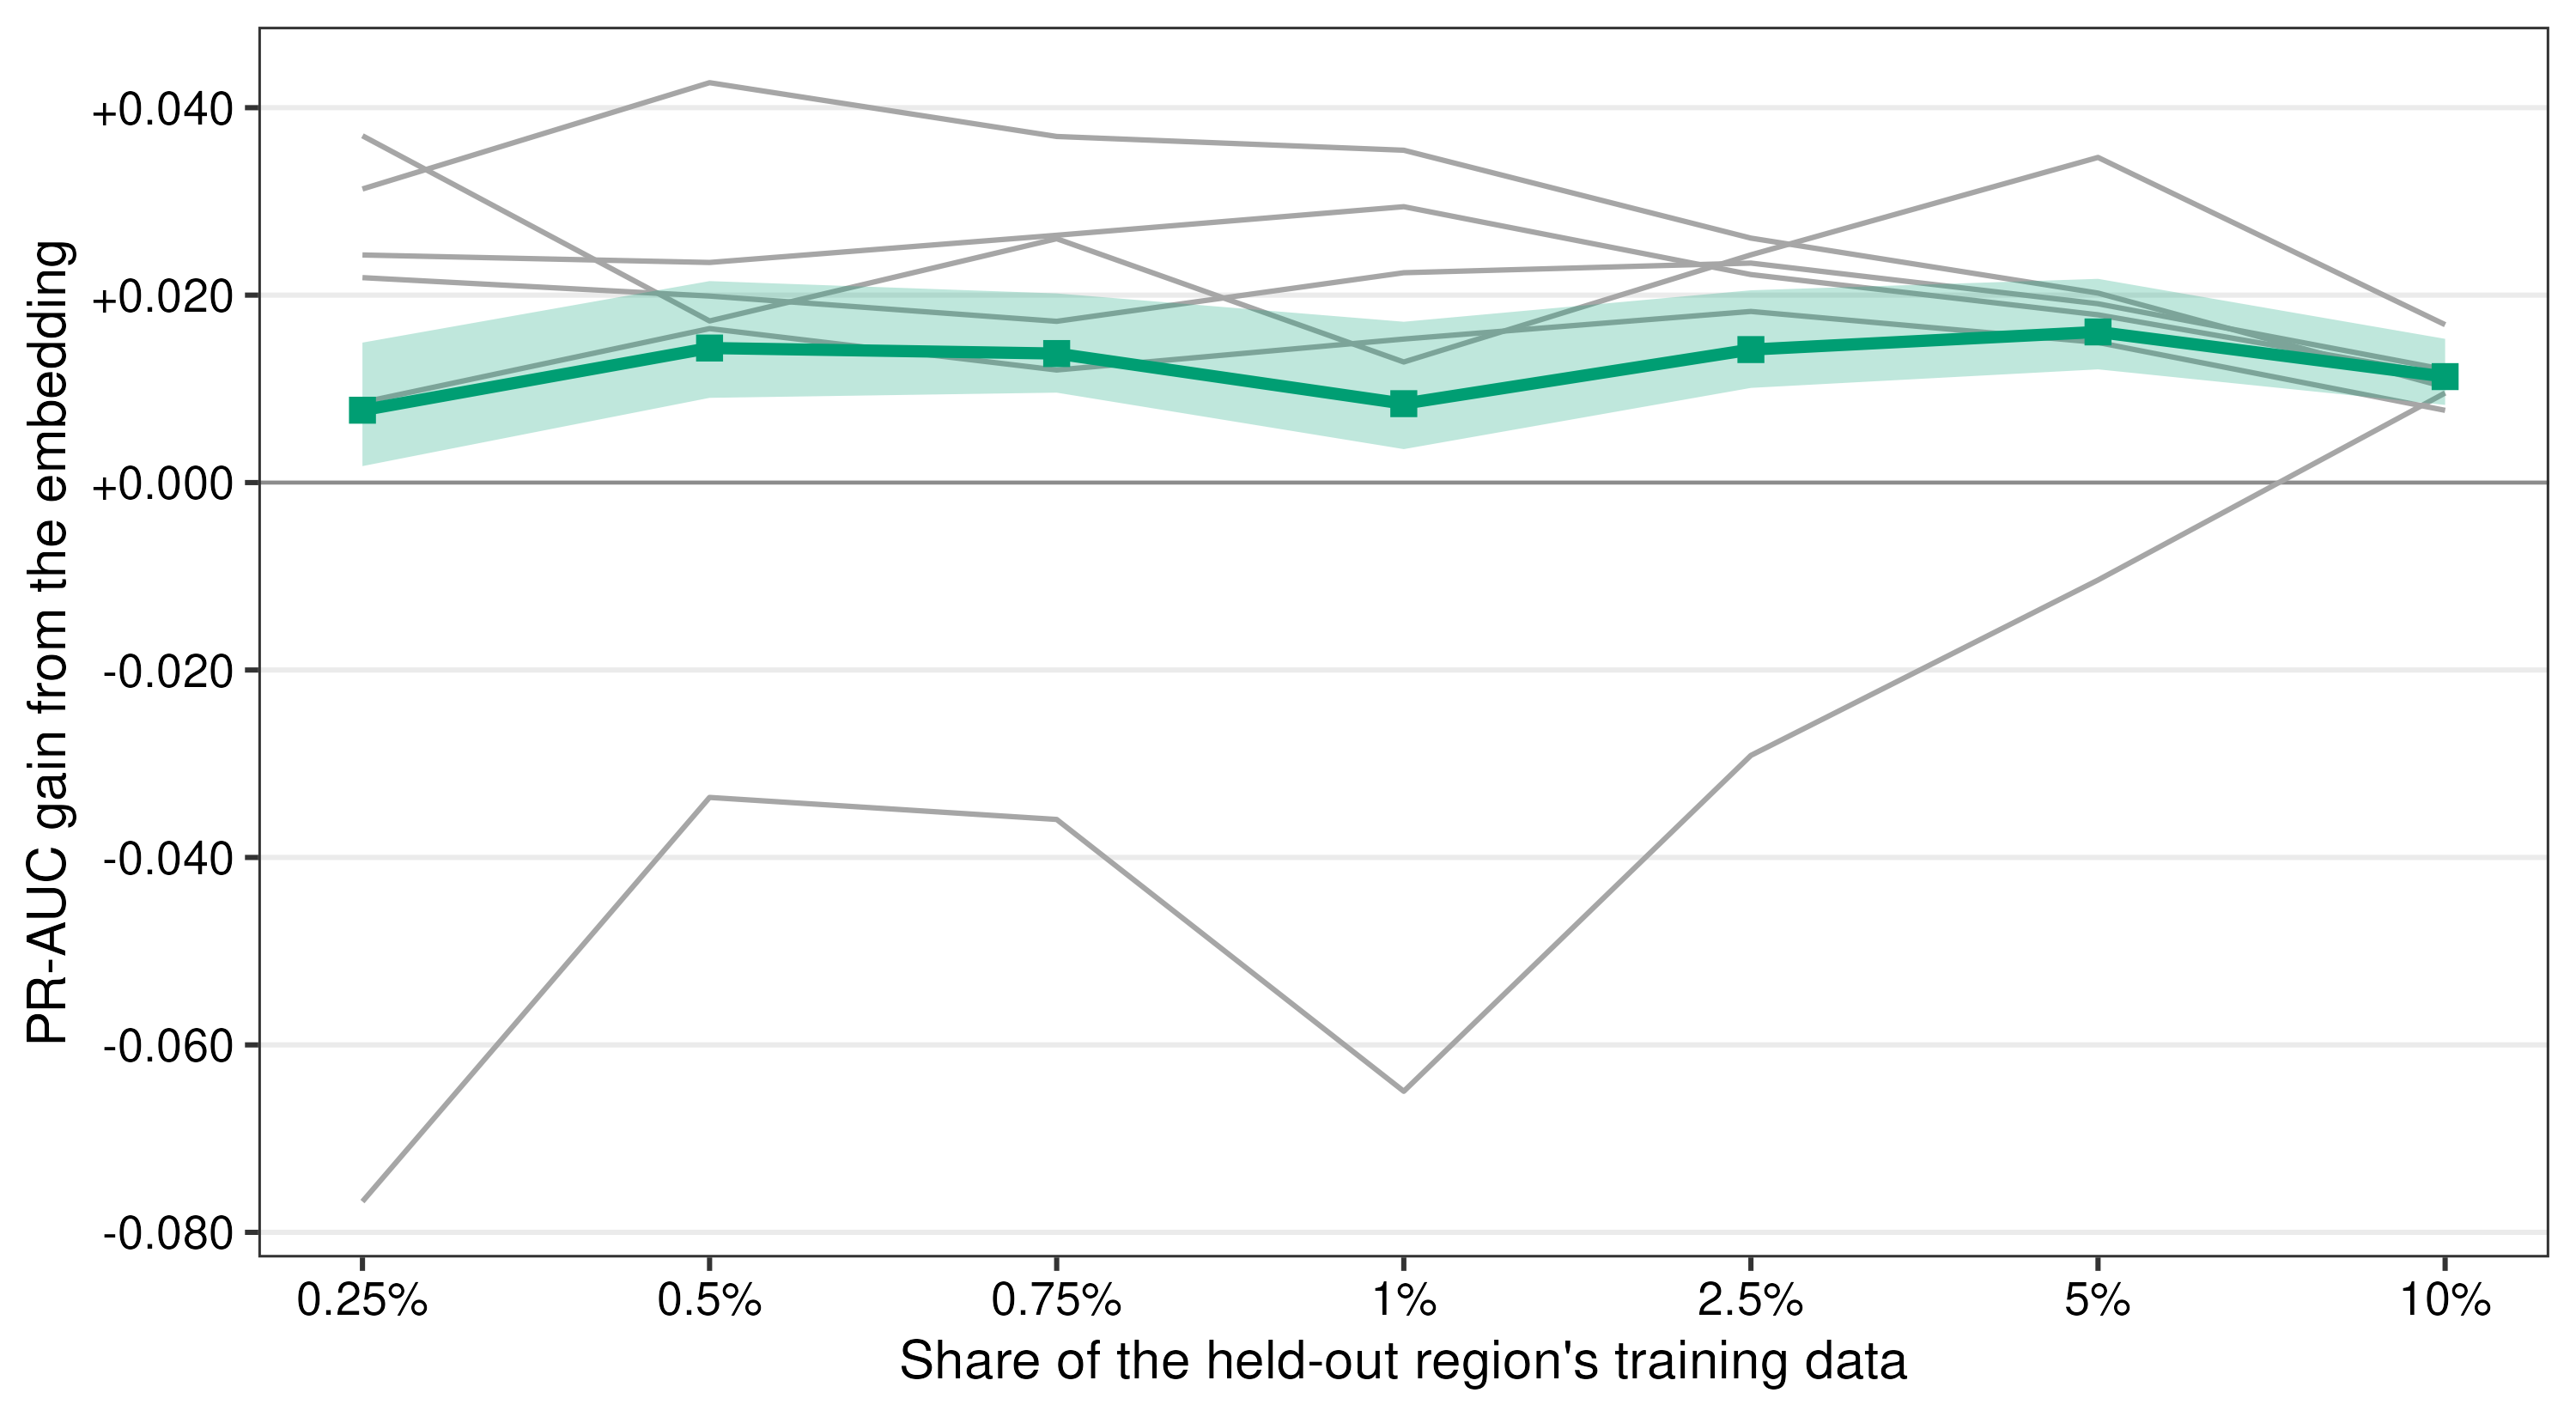
\includegraphics[width=\textwidth]{figures/fig_boot_shares_M.png}
\caption{Gain from adding the frozen embedding when the forecaster sees only a small share of the held-out region's training data (temporal test, PR-AUC). Teal line and band show the mean over the six held-out regions with its 95\% spatial-block bootstrap interval; gray lines show individual regions. Each point averages three encoder seeds and five random draws of the training share.}
\label{fig:boot_shares}
\end{figure}


\section{2022 Russia-Ukraine War}
\label{sec:ukraine}
In Section~\ref{sec:finetune}, I show that the pretrained encoder can be used for transfer learning in new regions. Here, I ground those findings by assessing whether the pretrained encoder improves out-of-sample prediction using the 2022 Russia-Ukraine War. This conflict offers a useful case for two reasons. First, the conflict unfolded outside of the training window, allowing me to assess the transformer on data that it has not been trained on. Second, the 2022 Russia-Ukraine War has been especially lethal, with estimates of 100,000 to 140,000 Ukrainian and 275,000 to 325,000 Russian military deaths through December 2025 \citep{jones2026grinding}. These features make the war a demanding test of whether the pretrained encoder is useful for forecasting violence in a new war.

To assess the model, I score the Europe hold-out models from Section~\ref{sec:finetune} on Ukraine's grid cells alone, without retraining. Ukraine contributes 13,200 test cell-months, 4,745 of them violent, constituting two-thirds of Europe's violent test cell-months. With 0.25 percent of Europe's training data, the fine-tuned encoder beats the network trained from scratch in Ukraine by +0.134 [+0.106, +0.161], more than twice its average across regions (+0.053), and it scores higher in all 15 seed and draw runs (Table~\ref{tab:ukraine_ft}). The advantage is also clear at 1 percent (+0.085 [+0.067, +0.101]) but is uneven at the other shares, ranging from $-$0.014 at 0.75 percent to +0.032 at 10 percent.\footnote{With 0.25 percent of the data, the fine-tuned encoder beats persistence in Ukraine (PR-AUC of 0.66, against 0.64 for persistence), while the network trained from scratch does not (0.52); from 0.5 percent on, the fine-tuned encoder scores 0.70 to 0.82.}


\begin{table}[t]
\centering
\caption{Fine-Tuned Pretrained Encoder Versus the Same Network Trained From Scratch, Ukraine}
\label{tab:ukraine_ft}
\scriptsize\setlength{\tabcolsep}{2.5pt}
\resizebox{\textwidth}{!}{\begin{tabular}{lccccccc}
\hline
& \multicolumn{7}{c}{Share of Europe's training data (\%)} \\
& 0.25 & 0.5 & 0.75 & 1 & 2.5 & 5 & 10 \\
\hline
\multicolumn{8}{l}{\textit{All parameters tuned}} \\
Ukraine & +0.134 & +0.022 & $-$0.014 & +0.085 & +0.009 & $-$0.004 & +0.032 \\
& [+0.106, +0.161] & [+0.010, +0.033] & [$-$0.024, $-$0.004] & [+0.067, +0.101] & [+0.001, +0.018] & [$-$0.013, +0.004] & [+0.026, +0.038] \\
Runs $>0$ (\%) & 100 & 53 & 47 & 73 & 60 & 53 & 80 \\
Europe (all cells) & +0.070 & $-$0.020 & $-$0.024 & +0.005 & +0.000 & $-$0.042 & +0.028 \\
\hline
\multicolumn{8}{l}{\textit{Top two layers tuned}} \\
Ukraine & +0.139 & +0.051 & +0.020 & +0.101 & $-$0.007 & +0.013 & +0.024 \\
& [+0.105, +0.169] & [+0.038, +0.065] & [+0.004, +0.036] & [+0.083, +0.118] & [$-$0.017, +0.004] & [+0.004, +0.021] & [+0.015, +0.032] \\
Runs $>0$ (\%) & 80 & 67 & 60 & 80 & 47 & 67 & 67 \\
Europe (all cells) & +0.045 & $-$0.012 & $-$0.053 & +0.019 & $-$0.053 & $-$0.037 & +0.006 \\
\hline
\end{tabular}}
\caption*{\footnotesize \textit{Note:} Entries are PR-AUC differences, fine-tuned pretrained encoder minus the same network trained from scratch, averaged over three encoder seeds and five draws of the training share. The models are the Europe hold-out models from Section~\ref{sec:finetune}, scored on Ukraine's 13,200 test cell-months (forecasts made January 2022 to April 2025) without retraining. Rows are grouped by fine-tuning arm: all parameters of the encoder and the output layer tuned (the arm in Section~\ref{sec:finetune}), and only the top two transformer layers and the output layer tuned. Runs $>0$ is the share of the 15 seed and draw runs in which the pretrained encoder scores higher in Ukraine. The Europe row is the same comparison across all of Europe's test cells.}
\end{table}

Figure~\ref{fig:ukraine_invasion} visualizes the forecasts during the first six months of the invasion.\footnote{I show the forecasts at 0.25 percent of Europe's training data, the share at which the fine-tuned encoder's advantage over the network trained from scratch in Ukraine is largest over the full test period. Table~\ref{tab:ukraine_ft} reports every share.} In these months, the forecast averaged across the 15 runs fine-tuned on 0.25 percent of Europe's training data identifies 465 of the 798 violent cell-months, against 466 for the averaged network trained from scratch at the same number of alerts, so in this window it beats persistence and matches the scratch network (PR-AUC of 0.626 against 0.624 and 0.571). Over the full test period the fine-tuned encoder pulls ahead of the scratch network (Table~\ref{tab:ukraine_ft}).
\begin{figure}[t]
\centering
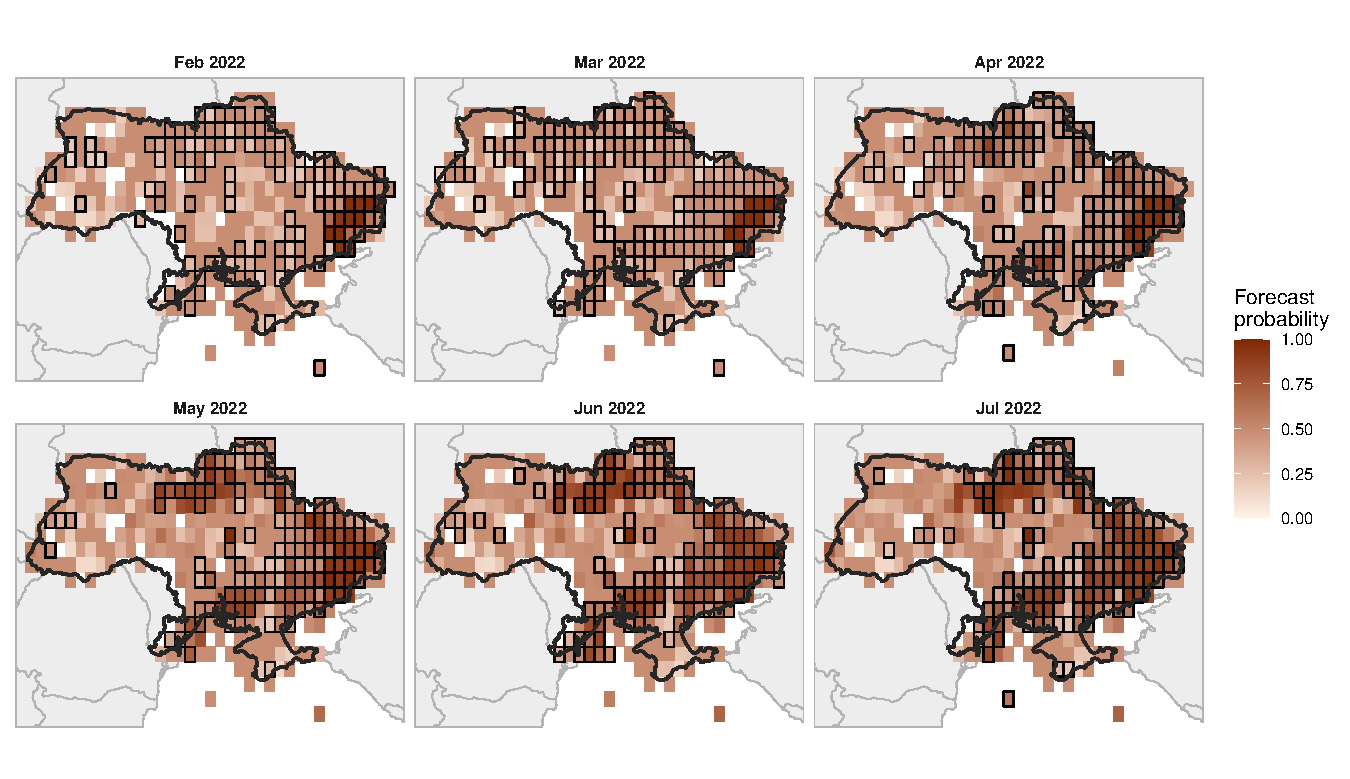
\includegraphics[width=\textwidth]{figures/fig_ukraine_f0025_full_1_invasion.pdf}
\caption{Forecasts of Violence in Ukraine, February to July 2022. Cells are 0.5-degree PRIO-GRID cells assigned to Ukraine. Shading is the forecast probability of any violent event in the month shown, from the pretrained encoder fine-tuned on 0.25 percent of Europe's training data, averaged over the 15 fine-tuned runs (three encoder seeds by five draws). Over the full test period, this averaged forecast has a PR-AUC of 0.76 in Ukraine, against 0.64 for persistence and 0.66 for the average single run; each forecast is made at the end of the previous month. Black outlines mark cells with at least one violent event that month. White cells are not in the Ukraine test sample. National borders are from Natural Earth (internationally recognized boundaries).}
\label{fig:ukraine_invasion}
\end{figure}

\subsection{Ukraine Forecast Maps}
\label{app:ukraine_maps}
Figure~\ref{fig:ukraine_alert_gain} shows where the fine-tuned encoder changes Ukraine forecasts at the two ends of the data-scarcity range. With 0.25 percent of Europe's training data the pretrained model adds correct alerts across most of the country, and with 10 percent the gains and losses roughly offset. This is the spatial counterpart of the $+0.134$ at 0.25 percent and $+0.032$ at 10 percent reported in Table~\ref{tab:ukraine_ft}.


\begin{figure}[!htbp]
\centering
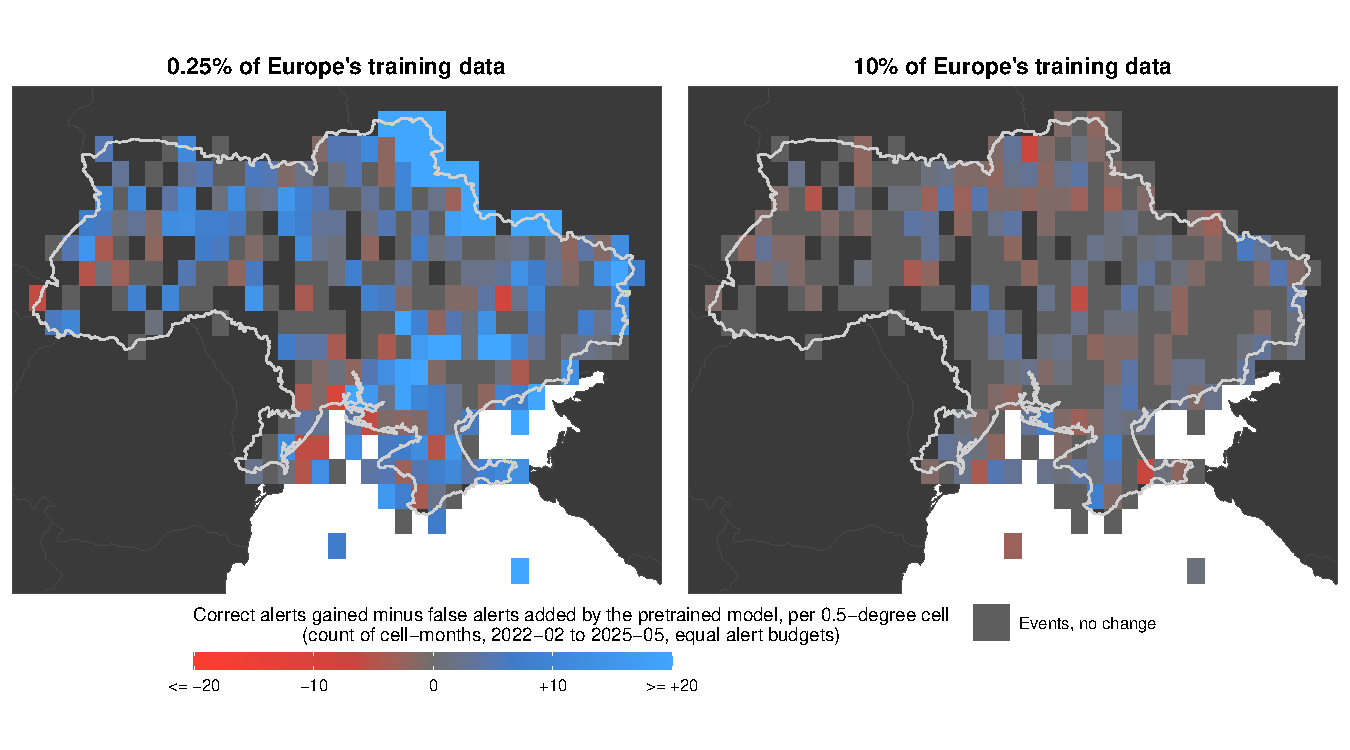
\includegraphics[width=\textwidth]{figures/fig_ukraine_alert_gain_full.pdf}
\caption{Where the pretrained encoder changes Ukraine forecasts, by the amount of local fine-tuning data. Each 0.5-degree cell is shaded by the number of correct alerts gained minus false alerts added by the pretrained, fine-tuned model relative to the same architecture trained from scratch, summed over the 40 target months February 2022 to May 2025. Both models flag the same number of cell-months, a budget equal to the 4,745 violent cell-months in the window, following the equal-budget convention of Figure~\ref{fig:cell_maps}. Blue marks cells where the pretrained model gains, red where it loses, on one symmetric scale shared by both panels. Counts beyond plus or minus 20 are clipped to the ends of the scale, which affects 28 of 660 cells. Gray marks cells with violent events but no change in alerts, and cells with neither events nor change are left as unshaded land. At 0.25 percent of Europe's training data the pretrained model gains in 175 cells and loses in 43, a net of 1,652 cell-months. At 10 percent it gains in 84 and loses in 73, a net of 84.}
\label{fig:ukraine_alert_gain}
\end{figure}


Figures~\ref{fig:ukraine_invasion}, \ref{fig:ukraine_counter}, \ref{fig:ukraine_south}, and~\ref{fig:ukraine_2024} display the forecasts during the invasion, the counteroffensives, the southern front, and the 2024 to 2025 fighting. These maps compare the averaged forecast from the pretrained encoder against persistence. The averaged forecast improves on persistence by +0.055 PR-AUC during the invasion (Figure~\ref{fig:ukraine_invasion}), +0.087 during the counteroffensives (Figure~\ref{fig:ukraine_counter}), +0.144 on the southern front (Figure~\ref{fig:ukraine_south}), and +0.171 from August 2024 to May 2025 (Figure~\ref{fig:ukraine_2024}). Over the full test period, the averaged forecast reaches a PR-AUC of 0.76, against 0.64 for persistence and 0.66 for the average single run. The gain over the averaged network trained from scratch grows over the war, from +0.001 during the invasion to +0.186, +0.244, and +0.264 in the three later periods.

\begin{figure}[!htbp]
\centering
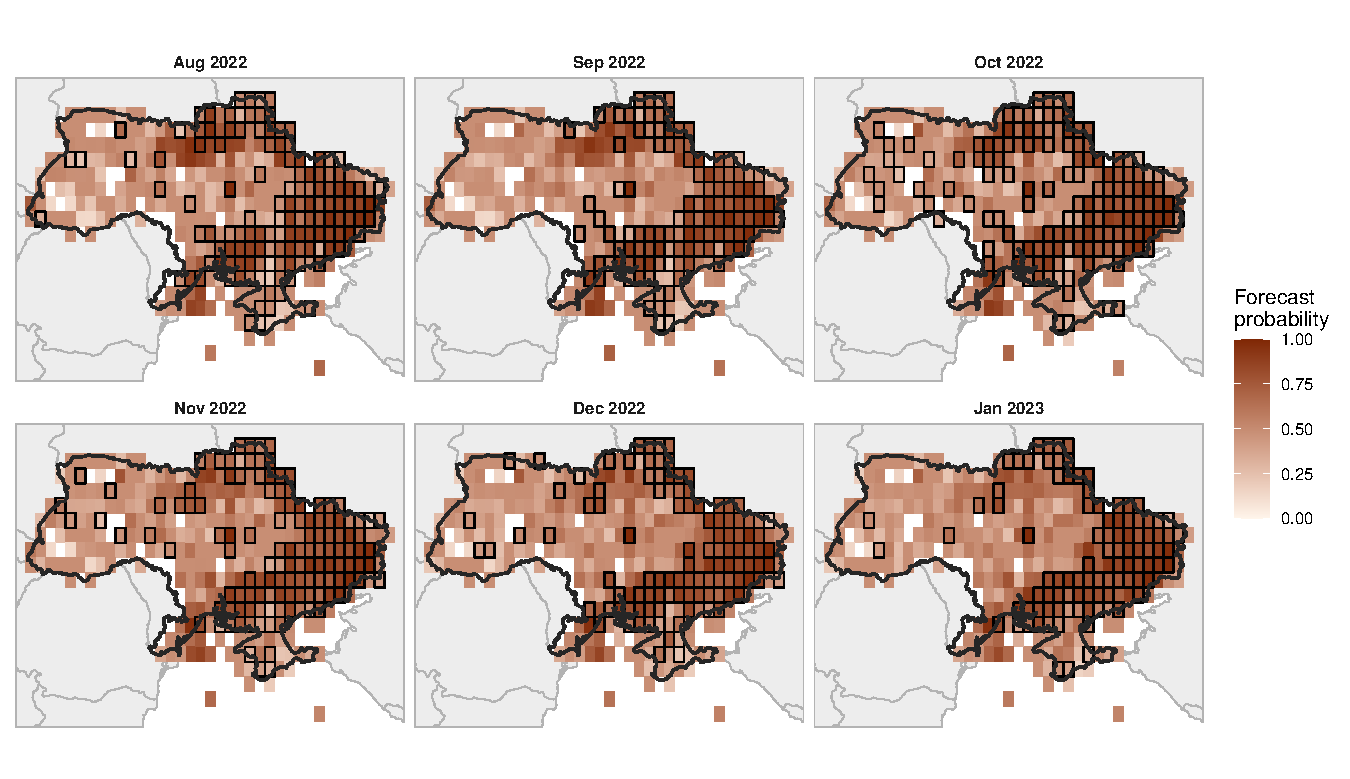
\includegraphics[width=\textwidth]{figures/fig_ukraine_f0025_full_2_counteroffensives.pdf}
\caption{Forecasts of Violence in Ukraine, August 2022 to January 2023. Cells are 0.5-degree PRIO-GRID cells assigned to Ukraine. Shading is the forecast probability of any violent event in the month shown, from the pretrained encoder fine-tuned on 0.25 percent of Europe's training data, averaged over the 15 fine-tuned runs (three encoder seeds by five draws). This averaged forecast has a PR-AUC of 0.76 in Ukraine, against 0.64 for persistence and 0.66 for the average single run; each forecast is made at the end of the previous month. Black outlines mark cells with at least one violent event that month. White cells are not in the Ukraine test sample. National borders are from Natural Earth (internationally recognized boundaries).}
\label{fig:ukraine_counter}
\end{figure}

\begin{figure}[!htbp]
\centering
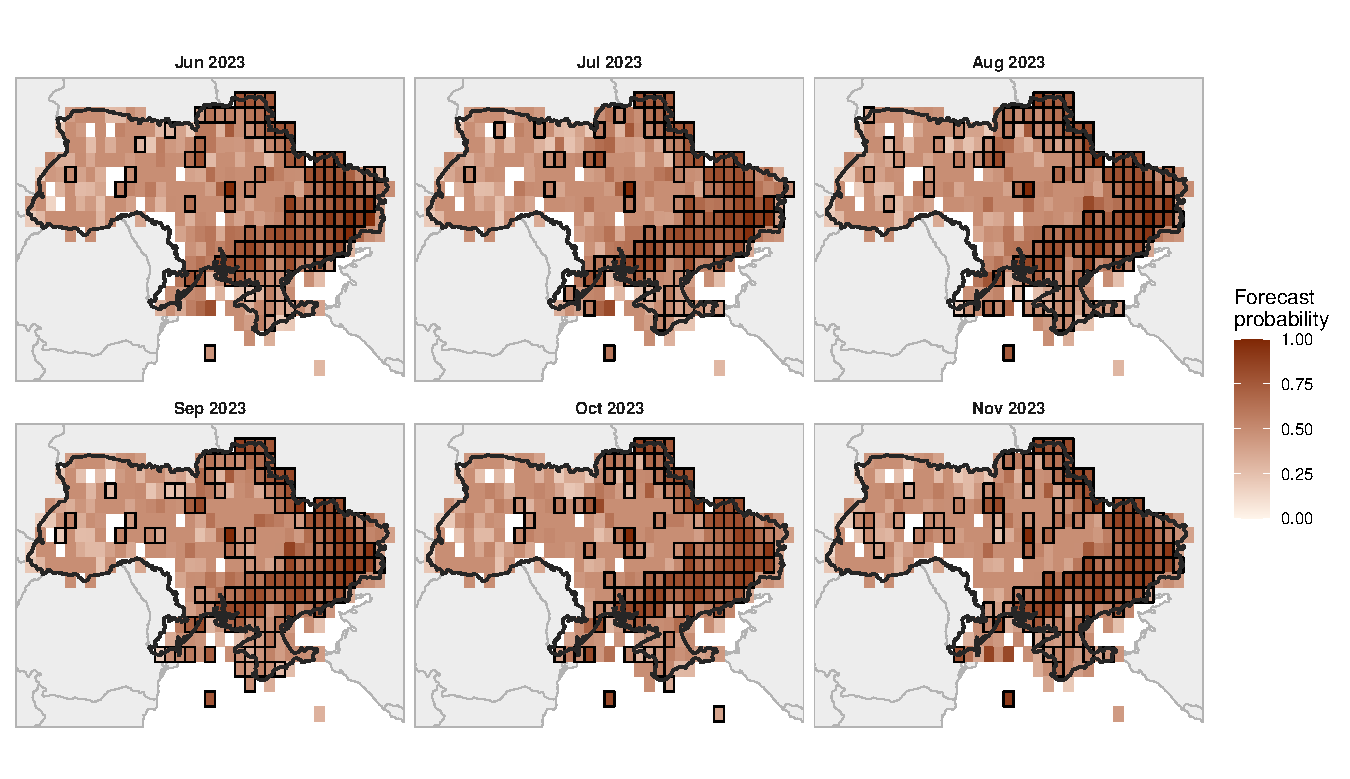
\includegraphics[width=\textwidth]{figures/fig_ukraine_f0025_full_3_southern_offensive.pdf}
\caption{Forecasts of Violence in Ukraine, June to November 2023. Cells are 0.5-degree PRIO-GRID cells assigned to Ukraine. Shading is the forecast probability of any violent event in the month shown, from the pretrained encoder fine-tuned on 0.25 percent of Europe's training data, averaged over the 15 fine-tuned runs (three encoder seeds by five draws). This averaged forecast has a PR-AUC of 0.76 in Ukraine, against 0.64 for persistence and 0.66 for the average single run; each forecast is made at the end of the previous month. Black outlines mark cells with at least one violent event that month. White cells are not in the Ukraine test sample. National borders are from Natural Earth (internationally recognized boundaries).}
\label{fig:ukraine_south}
\end{figure}

\begin{figure}[!htbp]
\centering
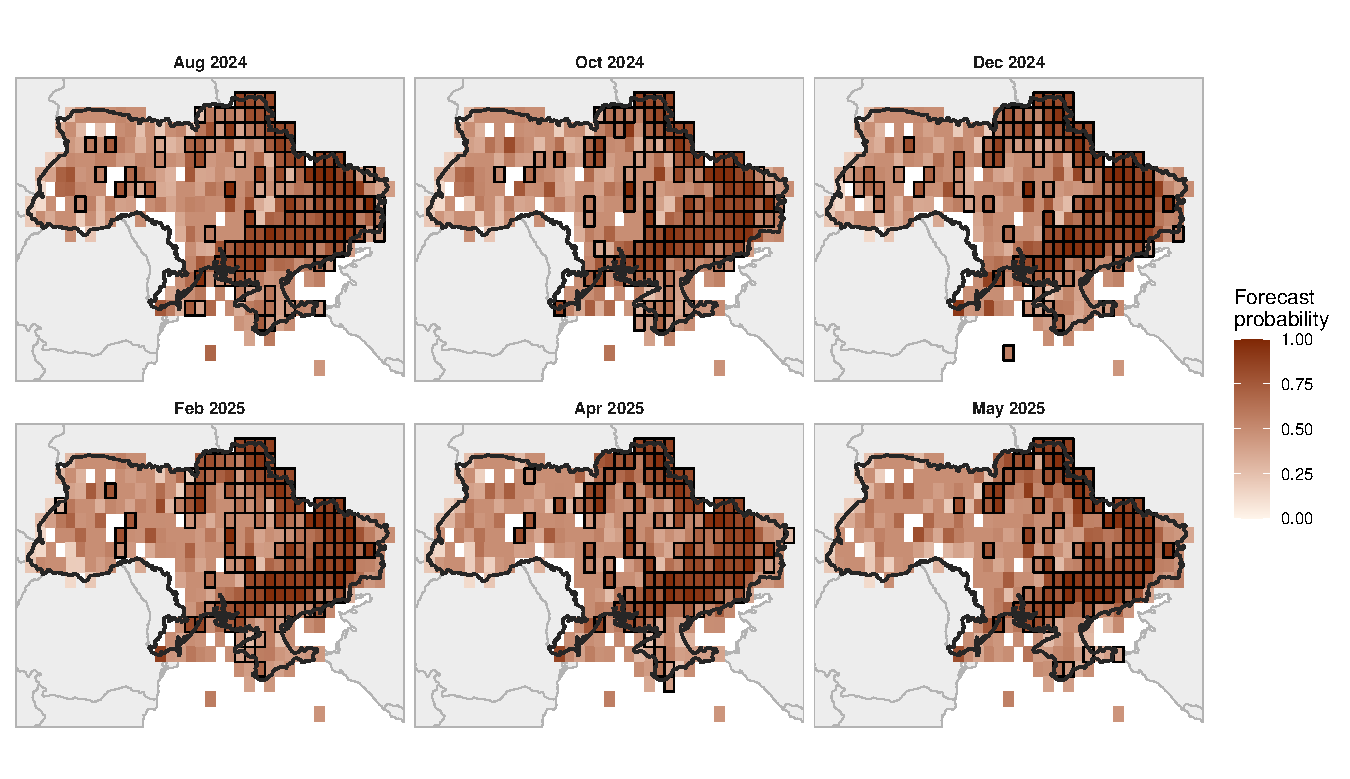
\includegraphics[width=\textwidth]{figures/fig_ukraine_f0025_full_4_2024_2025.pdf}
\caption{Forecasts of Violence in Ukraine, August 2024 to May 2025 (every second month, then April and May 2025). Cells are 0.5-degree PRIO-GRID cells assigned to Ukraine. Shading is the forecast probability of any violent event in the month shown, from the pretrained encoder fine-tuned on 0.25 percent of Europe's training data, averaged over the 15 fine-tuned runs (three encoder seeds by five draws). This averaged forecast has a PR-AUC of 0.76 in Ukraine, against 0.64 for persistence and 0.66 for the average single run; each forecast is made at the end of the previous month. Black outlines mark cells with at least one violent event that month. White cells are not in the Ukraine test sample. National borders are from Natural Earth (internationally recognized boundaries).}
\label{fig:ukraine_2024}
\end{figure}
\section{Transfer Within Other Domains}
\label{app:transformers_other_domains}
In this section, I (a) construct transformers from other high-dimensional data sources and (b) discuss the Brazil mortality transfer framework in further detail. 
\subsection{Other Data Sources}
\label{app:domains}
In the main text, I show that encoders can be developed from high-dimensional data and used for transfer learning with spatial political violence. Here, I replicate the main analyses using validated turnout from the Cooperative Election Study (CES) \citep{kuriwaki2026ces}, crime incidents from the Crime Open Database \citep{ashby2019code}, and dengue outbreaks in Brazil \citep{cox2024arbovirus}. These analyses follow the same set-up as the main text, but the held-out units follow the geography of each data source. Specifically, the CES analysis holds out each of the nine U.S.\ census divisions, the crime analysis holds out each of five U.S.\ cities (Austin, Boston, Los Angeles, St.\ Louis, and Seattle), and the dengue analysis holds out each of Brazil's five macro-regions (North, Northeast, Southeast, South, and Center-West).

Table~\ref{tab:domains} displays the results for the held-out units when only a small share of their training data is available. As in the main analyses, with 0.25 percent of the held-out unit's training data, the pretrained encoders for CES turnout, crime, and dengue outperform their comparisons. Specifically, for the CES, the fine-tuned encoder beats the network trained from scratch, and the embedding beats the base model, in eight of nine census divisions. For crime, the fine-tuned encoder wins in five of five cities and the embedding in four of five, and for dengue, the fine-tuned encoder wins in five of five regions and the embedding in four of five. For the CES and crime, the gains largely persist at larger data shares, although the fine-tuning gain shrinks to about zero at 10 percent. For dengue, the fine-tuning gain disappears after 0.25 percent, and the embedding gains are small and mixed.

\begin{table}[!htbp]
\centering
\caption{Limited-Data Transfer for Turnout, Crime, and Dengue}
\label{tab:domains}
\small
\begin{tabular}{llccccccc}
\hline
 & & \multicolumn{7}{c}{Share of the held-out unit's training data (\%)} \\
Domain & Comparison & 0.25 & 0.5 & 0.75 & 1 & 2.5 & 5 & 10 \\
\hline
CES turnout & Fine-tuned vs.\ scratch & +0.033 & +0.036 & +0.017 & +0.029 & +0.019 & +0.004 & +0.001 \\
 & Units $>0$ & 8/9 & 9/9 & 8/9 & 9/9 & 8/9 & 7/9 & 6/9 \\
CES turnout & Embedding vs.\ base & +0.012 & +0.017 & +0.017 & +0.015 & +0.011 & +0.008 & +0.005 \\
 & Units $>0$ & 8/9 & 9/9 & 9/9 & 9/9 & 9/9 & 9/9 & 7/9 \\
Crime & Fine-tuned vs.\ scratch & +0.085 & +0.078 & +0.086 & +0.058 & +0.019 & +0.021 & $-$0.006 \\
 & Units $>0$ & 5/5 & 5/5 & 4/5 & 5/5 & 4/5 & 4/5 & 0/5 \\
Crime & Embedding vs.\ base & +0.014 & +0.035 & +0.032 & +0.032 & +0.048 & +0.040 & +0.041 \\
 & Units $>0$ & 4/5 & 5/5 & 5/5 & 5/5 & 5/5 & 5/5 & 5/5 \\
Dengue & Fine-tuned vs.\ scratch & +0.059 & $-$0.006 & +0.006 & $-$0.006 & $-$0.007 & $-$0.007 & $-$0.008 \\
 & Units $>0$ & 5/5 & 2/5 & 2/5 & 2/5 & 1/5 & 1/5 & 1/5 \\
Dengue & Embedding vs.\ base & +0.011 & +0.007 & $-$0.000 & +0.006 & +0.003 & +0.004 & +0.009 \\
 & Units $>0$ & 4/5 & 4/5 & 2/5 & 2/5 & 3/5 & 3/5 & 3/5 \\
\hline
\end{tabular}
\caption*{\footnotesize \textit{Note:} Entries are PR-AUC differences averaged over the held-out units (nine census divisions for the CES, five cities for crime, five regions for dengue), three encoder seeds (123, 456, 789) and five draws of the training share. \emph{Fine-tuned vs.\ scratch} compares the fine-tuned pretrained encoder with the same network trained from scratch. \emph{Embedding vs.\ base} compares a gradient-boosted forecaster with and without the frozen embedding. \emph{Units $>0$} counts held-out units whose mean difference is positive.}
\end{table}
\subsection{Mapping Brazilian Mortality Records to the Conflict Vocabulary}
\label{app:vocab}
In the main text, I assess whether the pretrained encoder can improve forecasting across four mortality outcomes in Brazil. Here, I list the decision rules used to map the Brazilian mortality records to the encoder's vocabulary. Table~\ref{tab:brazil_vocab} lists those decisions. The labels follow how ACLED codes comparable events in Brazil, so each death is expressed in terms the encoder saw during pretraining.

To format the data, I assign each death to its municipality of occurrence and then to the 0.5-degree PRIO-GRID cell that holds that municipality's IBGE centroid.\footnote{When the municipality of occurrence is missing, I use the municipality of residence.} The analysis includes every cell that holds at least one municipality centroid. Figure~\ref{fig:brazil_deaths_map} displays a heat map of the total data. Table~\ref{tab:brazil_summary} displays summary statistics of the outcomes.

% ADDED 2026-11-06: generated by scripts/crossdomain/brazil_descriptives.py and fig_brazil_deaths_map.R (pipeline task br_desc)
\begin{figure}[!htbp]
\centering
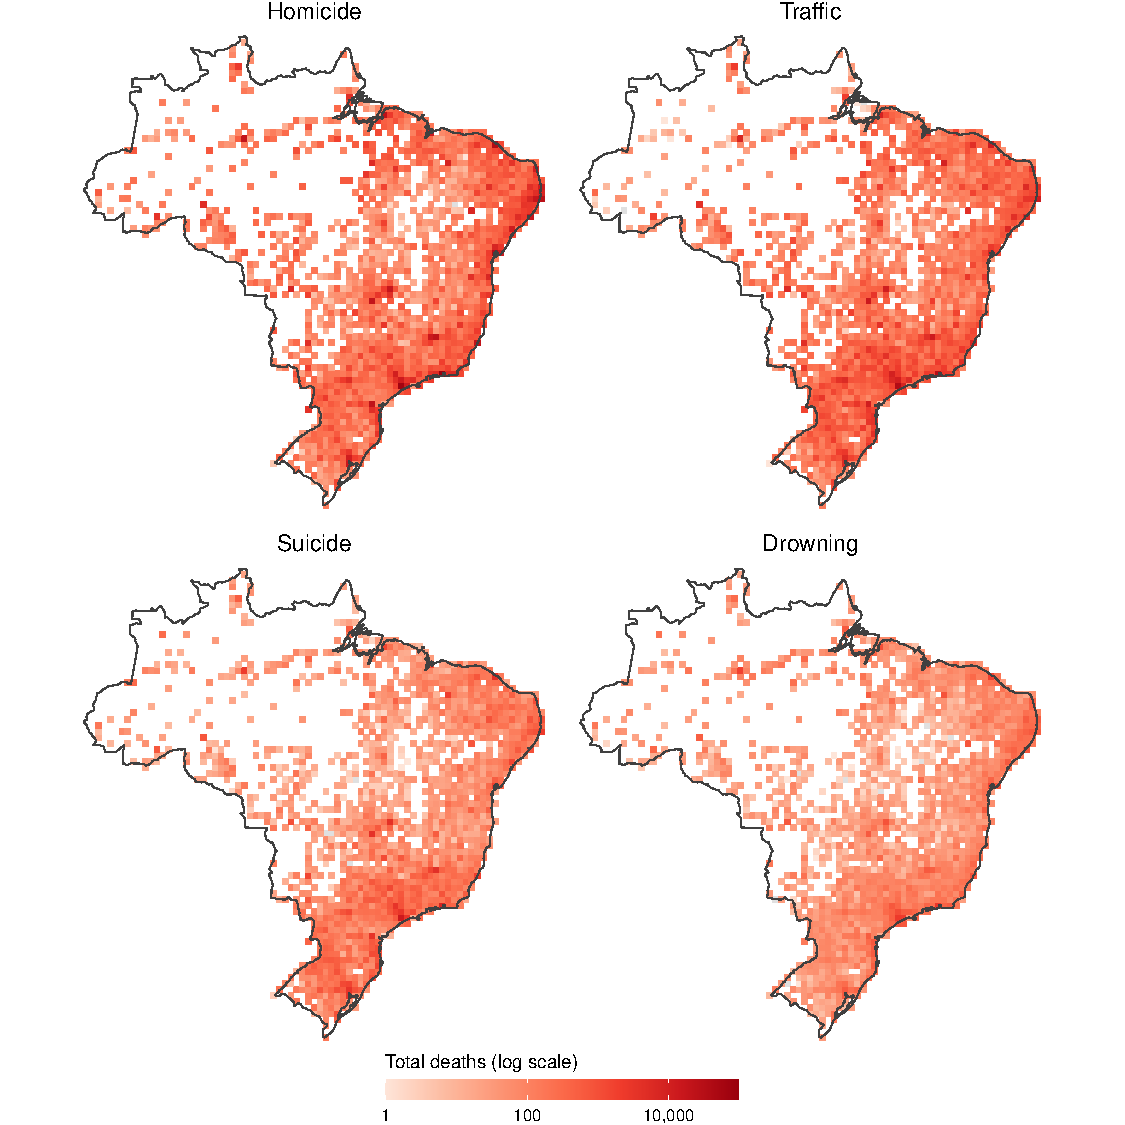
\includegraphics[width=0.85\textwidth]{figures/fig_brazil_deaths_map.pdf}
\caption{Total deaths per 0.5-degree PRIO-GRID cell from February 2001 to December 2024, by outcome, on one log scale shared by the four panels. Gray cells recorded no deaths. Unshaded areas inside Brazil are cells with no municipality centroid, which are not in the analysis. Source: SIM death records \citep{sim_datasus}.}
\label{fig:brazil_deaths_map}
\end{figure}

% Generated by scripts/crossdomain/brazil_descriptives.py from outputs/crossdomain/brazil_summary.csv. Do not edit by hand.
\begin{table}[!htbp]
\centering
\caption{Summary Statistics for the Four Brazilian Mortality Outcomes}
\label{tab:brazil_summary}
\small
\begin{tabular}{llrrrrr}
\hline
Outcome & Period & Total deaths & Mean & SD & Any death (\%) & Max \\
\hline
Homicide & Training & 1,068,577 & 3.01 & 16.96 & 44.0 & 851 \\
 & Test & 130,856 & 2.53 & 9.42 & 49.6 & 330 \\
\hline
Traffic & Training & 743,321 & 2.10 & 7.00 & 46.5 & 220 \\
 & Test & 103,321 & 2.00 & 4.90 & 51.6 & 120 \\
\hline
Suicide & Training & 202,702 & 0.57 & 2.07 & 26.0 & 77 \\
 & Test & 48,801 & 0.94 & 2.63 & 36.8 & 62 \\
\hline
Drowning & Training & 111,593 & 0.31 & 0.96 & 18.8 & 39 \\
 & Test & 14,546 & 0.28 & 0.80 & 18.5 & 24 \\
\hline
\end{tabular}
\caption*{\footnotesize \textit{Note:} Statistics are for the outcome the forecasters predict, deaths in month $t+1$, over 1,478 PRIO-GRID cells. The training period covers forecast origins from January 2001 to December 2020 (354,720 cell-months) and the test period covers origins from January 2022 to November 2024 (51,730 cell-months). Mean, SD, and Max are deaths per cell-month. Any death is the share of cell-months with at least one death. Source: SIM death records \citep{sim_datasus}.}
\end{table}



The cells form a monthly panel from January 2000 to December 2024. I use rows from January 2001 onward, so every row has 12 months of history. For the test, I use the medium-sized encoders with the Americas held out, meaning that the encoders never saw events from the Americas, including Brazil. The training period rows run from January 2001 to December 2020, with validation data for 2021. The test covers the forecast origins from January 2022 to November 2024. 

For the training shares, I use 0.25, 1, 5, 10, and 100 percent of the data with five random draws per share for all shares below 100 percent. I use the same baseline features as the conflict models rebuilt from Brazilian deaths plus the PRIO-GRID covariates. The forecaster is XGBoost with a Poisson objective function. A cell with zero deaths in the previous 12 months gets an embedding of zero, the same rule as the conflict evaluation. 

For the outcome, I use the count of deaths in month $t+1$ scored with Poisson deviance. Gains in forecasting are relative deviance reductions. For the uncertainty quantification, I use a two-way bootstrap that resamples grid cells and the 15 seed and draw pairs with 1,000 replicates and seed 123. Comparisons across outcomes use the same resampled cells and pairs, so differences between outcomes are paired. 


\begin{table}[!htbp]
\centering
\caption{ICD-10 Cause of Death Mapped to the Pretrained Encoder's Vocabulary}
\label{tab:brazil_vocab}
\small
\begin{tabular}{lllll}
\hline
SIM record & event\_type & sub\_event\_type & actor1 (type) & actor2 (type) \\
\hline
Assault & Violence against & Attack & Unidentified Armed & Civilians (Brazil) \\
(X85--Y09) & civilians & & Group (Brazil) & \\
 & & & \textit{political militia} & \textit{civilians} \\
\hline
Assault by firearm & Violence against & Attack & Unidentified Gang & Civilians (Brazil) \\
(X93--X95), male & civilians & & (Brazil) & \\
victim aged 15--29 & & & \textit{political militia} & \textit{civilians} \\
\hline
Legal intervention & Battles & Armed clash & Military Forces of & Unidentified Gang \\
(Y35) & & & Brazil, Military Police & (Brazil) \\
 & & & \textit{state} & \textit{political militia} \\
\hline
\end{tabular}
\caption*{\footnotesize \textit{Note}: One event per death. The firearm row applies only under the rich specification used in the main results. Military Police actor names are period-specific, following ACLED's own naming (2016--2018, 2019--2022, 2023--). The fatalities bin is ``1--2'' for every record. The civilian-death bin is ``1--2'' for assaults and ``0'' for legal intervention. Suicide, traffic, and drowning deaths are coded with the assault row. Vocabulary ids come from the encoder's own \texttt{vocab\_super.json}; no Brazil-specific vocabulary is introduced.}
\end{table}


\begin{table}[!htbp]
\centering
\caption{Frozen Conflict Embedding Applied to Homicides in Brazil}
\label{tab:brazil}
\small
\begin{tabular}{lccccc}
\hline
& \multicolumn{5}{c}{Share of the training data (\%)} \\
Comparison & 0.25 & 1 & 5 & 10 & 100 \\
\hline
Pretrained vs.\ random encoder & +11.1 & +5.7 & +3.8 & +3.6 & +2.8 \\
& [+6.2, +16.7] & [+4.2, +7.6] & [+3.1, +4.4] & [+3.0, +4.1] & [+2.0, +3.4] \\
Pretrained vs.\ base & +2.9 & +6.8 & +6.1 & +6.0 & +8.5 \\
& [$-$2.7, +6.4] & [+5.8, +7.8] & [+5.4, +6.8] & [+5.4, +6.6] & [+5.4, +13.6] \\
Random encoder vs.\ base & $-$9.6 & +1.1 & +2.4 & +2.5 & +5.9 \\
& [$-$17.9, $-$3.7] & [$-$1.1, +2.7] & [+1.8, +3.1] & [+2.0, +3.0] & [+2.7, +11.3] \\
\hline
\end{tabular}
\end{table}

% ADDED 2026-10-29 by Claude at Jared's request: placebo gradient figure for the Section 5 falsification evidence.
% Source (Roar): outputs/placebo_gradient_M/fig_placebo_gradient_M.pdf, built by scripts/phase4_scaling/fig_placebo_gradient.R from outputs/crossdomain/xd_placebo_boot_v3M.csv via launch_placebo_gradient.sbatch (job 56857810, account open).
\begin{figure}[!htbp]
\centering
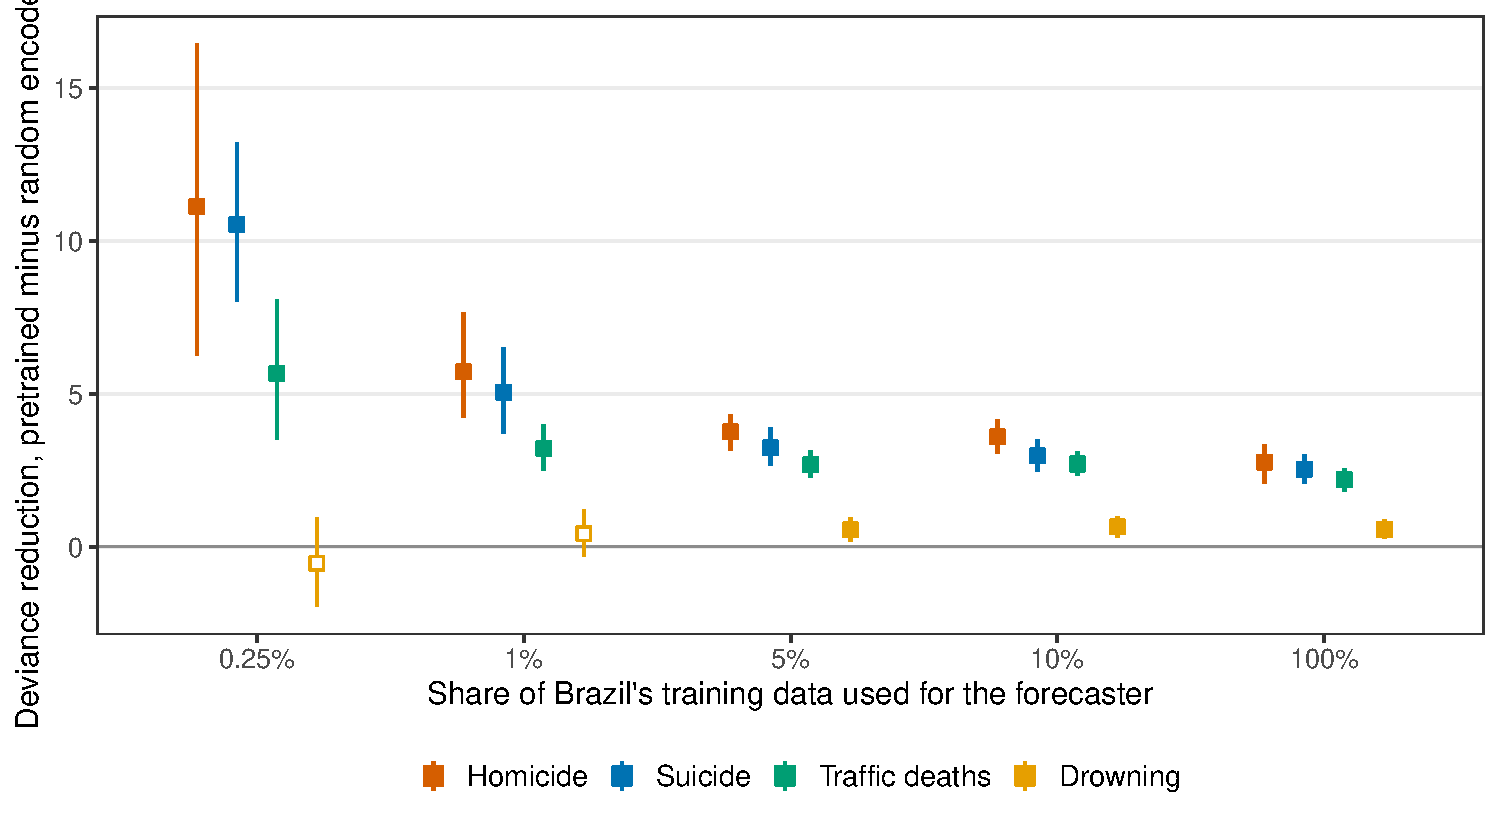
\includegraphics[width=\textwidth]{figures/fig_placebo_gradient.pdf}
\caption{Placebo gradient for the Brazil cross-domain test. Each square is the relative reduction in Poisson deviance from adding the frozen conflict embedding to the gradient-boosted forecaster, measured against the same forecaster with a randomly initialized encoder of the same architecture, by outcome and by the share of Brazil's training data used to train the forecaster. Squares are means over three encoder seeds and five draws of the training share, one draw with all data, and bars are 95\% paired bootstrap intervals that resample test cells and seed-draw pairs. Filled squares mark intervals that exclude zero and hollow squares mark intervals that include zero. Homicide is the target outcome and the other three are placebos.}
\label{fig:placebo_gradient}
\end{figure}

Against a randomly initialized encoder with the same architecture, at 0.25 percent of Brazil's training data the pretrained encoder reduces Poisson deviance by 11.1 percent for homicides, 10.5 percent for suicides, and 5.7 percent for traffic deaths, while drowning is slightly worse at $-$0.5 percent, the only interval to include zero.


\section{Bootstrap Intervals}
\label{app:bootstrap}
% MOVED from main-text footnote 2026-10-20 (Claude)
Training the encoder with multiple seeds allows me to gauge how much the results vary across runs \citep[see][for discussion of transformers varying by random initialization]{dodge2020finetuning, mosbach2021stability, sellam2022multiberts}.

% NOTES 2026-10-21 (Claude): my draft prose removed (see Overleaf History); write this in your own words. Numbers are from the OLD encoders.
\begin{itemize}
\item What. Paired cluster bootstrap, 1,000 replicates, resampling $5^\circ \times 5^\circ$ blocks of cells (main) or single cells (check).
\item Where. Table~\ref{tab:boot_main} has the three main comparisons by region. Table~\ref{tab:boot_shares} and Figure~\ref{fig:boot_share_regions} have the limited-data comparison at every share. Figure~\ref{fig:boot_persistence} has the gap over persistence.
\item Caveat to state. Intervals condition on the fitted models, encoder seeds and training draws, so they capture uncertainty from the test sample, not from retraining.
\end{itemize}
% UPDATED 2026-10-26 (Claude): Panels A and B = M full-source (bootstrap_ci_M_fullsrc_{block5,cell}.csv). Panel C M full-source (bootstrap_ci_M_fullsrc_{block5,cell}_rand.csv, job 56803740).
\begin{table}[!htbp]
\centering\footnotesize
\caption{Bootstrap intervals for the main comparisons (temporal test, PR-AUC differences)}
\label{tab:boot_main}
\begin{tabular}{lccc}
\hline
Held-out region & Estimate & 95\% interval, $5^\circ$ blocks & 95\% interval, single cells \\
\hline
\multicolumn{4}{l}{\textit{A. Base + embedding minus persistence}} \\
Africa & +0.304 & [+0.288, +0.320] & [+0.298, +0.310] \\
Americas & +0.345 & [+0.335, +0.355] & [+0.340, +0.351] \\
Asia-Pacific & +0.307 & [+0.271, +0.330] & [+0.294, +0.318] \\
Europe & +0.275 & [+0.235, +0.295] & [+0.263, +0.287] \\
MENA & +0.311 & [+0.283, +0.342] & [+0.296, +0.323] \\
South Asia & +0.317 & [+0.276, +0.331] & [+0.302, +0.329] \\
All regions & +0.310 & [+0.296, +0.317] & [+0.305, +0.314] \\
\hline
\multicolumn{4}{l}{\textit{B. Base + embedding minus base}} \\
Africa & +0.010 & [+0.008, +0.013] & [+0.009, +0.012] \\
Americas & +0.006 & [+0.002, +0.010] & [+0.004, +0.008] \\
Asia-Pacific & +0.031 & [+0.021, +0.042] & [+0.023, +0.038] \\
Europe & +0.013 & [$-$0.001, +0.022] & [+0.006, +0.021] \\
MENA & +0.005 & [+0.002, +0.011] & [+0.003, +0.008] \\
South Asia & +0.010 & [+0.005, +0.019] & [+0.006, +0.014] \\
All regions & +0.013 & [+0.009, +0.015] & [+0.011, +0.014] \\
\hline
\multicolumn{4}{l}{\textit{C. Pretrained minus random-weight encoder}} \\
Africa & +0.003 & [+0.001, +0.005] & [+0.002, +0.004] \\
Americas & +0.001 & [$-$0.000, +0.003] & [$-$0.000, +0.003] \\
Asia-Pacific & +0.019 & [+0.009, +0.028] & [+0.013, +0.025] \\
Europe & +0.001 & [$-$0.003, +0.007] & [$-$0.003, +0.006] \\
MENA & +0.000 & [$-$0.002, +0.002] & [$-$0.002, +0.002] \\
South Asia & +0.002 & [$-$0.002, +0.006] & [$-$0.001, +0.005] \\
All regions & +0.005 & [+0.002, +0.007] & [+0.003, +0.006] \\
\hline
\end{tabular}
\begin{minipage}{0.92\textwidth}\footnotesize\vspace{0.5ex}
Notes. Estimates are means over three encoder seeds; persistence is violence in month $t$. Intervals are 95\% percentile intervals from 1,000 paired bootstrap replicates that resample test units within each held-out region, keeping all test months of a unit together and applying the same draw to every model and seed. Units are $5^\circ \times 5^\circ$ blocks of grid cells or single grid cells. Intervals hold the fitted models fixed. All regions is the equal-weight mean of the six regions.
\end{minipage}
\end{table}

% UPDATED 2026-10-26 (Claude): M full-source, bootstrap_ci_M_fullsrc_block5_shares.csv (job 56803741).
\begin{table}[!htbp]
\centering\scriptsize\setlength{\tabcolsep}{2.5pt}
\caption{Gain from the embedding with limited local data: estimates and 95\% spatial-block bootstrap intervals}
\label{tab:boot_shares}
\resizebox{\textwidth}{!}{\begin{tabular}{lccccccc}
\hline
 & \multicolumn{7}{c}{Share of the held-out region's training data} \\
Held-out region & 0.25\% & 0.5\% & 0.75\% & 1\% & 2.5\% & 5\% & 10\% \\
\hline
Africa & +0.024 & +0.023 & +0.026 & +0.029 & +0.022 & +0.018 & +0.011 \\
 & [+0.017, +0.031] & [+0.016, +0.033] & [+0.021, +0.032] & [+0.024, +0.036] & [+0.018, +0.026] & [+0.014, +0.022] & [+0.009, +0.015] \\[2pt]
Americas & +0.022 & +0.020 & +0.017 & +0.022 & +0.023 & +0.019 & +0.012 \\
 & [+0.014, +0.029] & [+0.014, +0.026] & [+0.012, +0.023] & [+0.018, +0.027] & [+0.020, +0.027] & [+0.015, +0.023] & [+0.008, +0.016] \\[2pt]
Asia-Pacific & +0.037 & +0.017 & +0.026 & +0.013 & +0.024 & +0.035 & +0.017 \\
 & [+0.012, +0.059] & [$-$0.006, +0.044] & [+0.006, +0.047] & [$-$0.012, +0.048] & [+0.003, +0.050] & [+0.017, +0.058] & [+0.006, +0.034] \\[2pt]
Europe & $-$0.077 & $-$0.034 & $-$0.036 & $-$0.065 & $-$0.029 & $-$0.010 & +0.010 \\
 & [$-$0.097, $-$0.044] & [$-$0.048, $-$0.012] & [$-$0.045, $-$0.017] & [$-$0.079, $-$0.039] & [$-$0.040, $-$0.013] & [$-$0.021, +0.010] & [$-$0.000, +0.022] \\[2pt]
MENA & +0.009 & +0.016 & +0.012 & +0.015 & +0.018 & +0.015 & +0.008 \\
 & [$-$0.003, +0.023] & [+0.011, +0.025] & [+0.004, +0.024] & [+0.008, +0.028] & [+0.013, +0.029] & [+0.010, +0.025] & [+0.004, +0.013] \\[2pt]
South Asia & +0.031 & +0.043 & +0.037 & +0.035 & +0.026 & +0.020 & +0.010 \\
 & [+0.019, +0.047] & [+0.027, +0.063] & [+0.025, +0.052] & [+0.025, +0.050] & [+0.018, +0.035] & [+0.013, +0.031] & [+0.002, +0.022] \\[2pt]
\hline
All regions & +0.008 & +0.014 & +0.014 & +0.008 & +0.014 & +0.016 & +0.011 \\
 & [+0.002, +0.015] & [+0.009, +0.021] & [+0.010, +0.020] & [+0.004, +0.017] & [+0.010, +0.021] & [+0.012, +0.022] & [+0.008, +0.015] \\[2pt]
\hline
\end{tabular}}
\begin{minipage}{0.98\textwidth}\footnotesize\vspace{0.5ex}
Notes. Base + embedding minus base, both trained on the stated share of the held-out region's training months. Means over three encoder seeds and five draws of the training share. Brackets are 95\% intervals from 1,000 paired bootstrap replicates resampling $5^\circ \times 5^\circ$ blocks of grid cells; they hold the fitted models fixed.
\end{minipage}
\end{table}

\begin{figure}[!htbp]
\centering
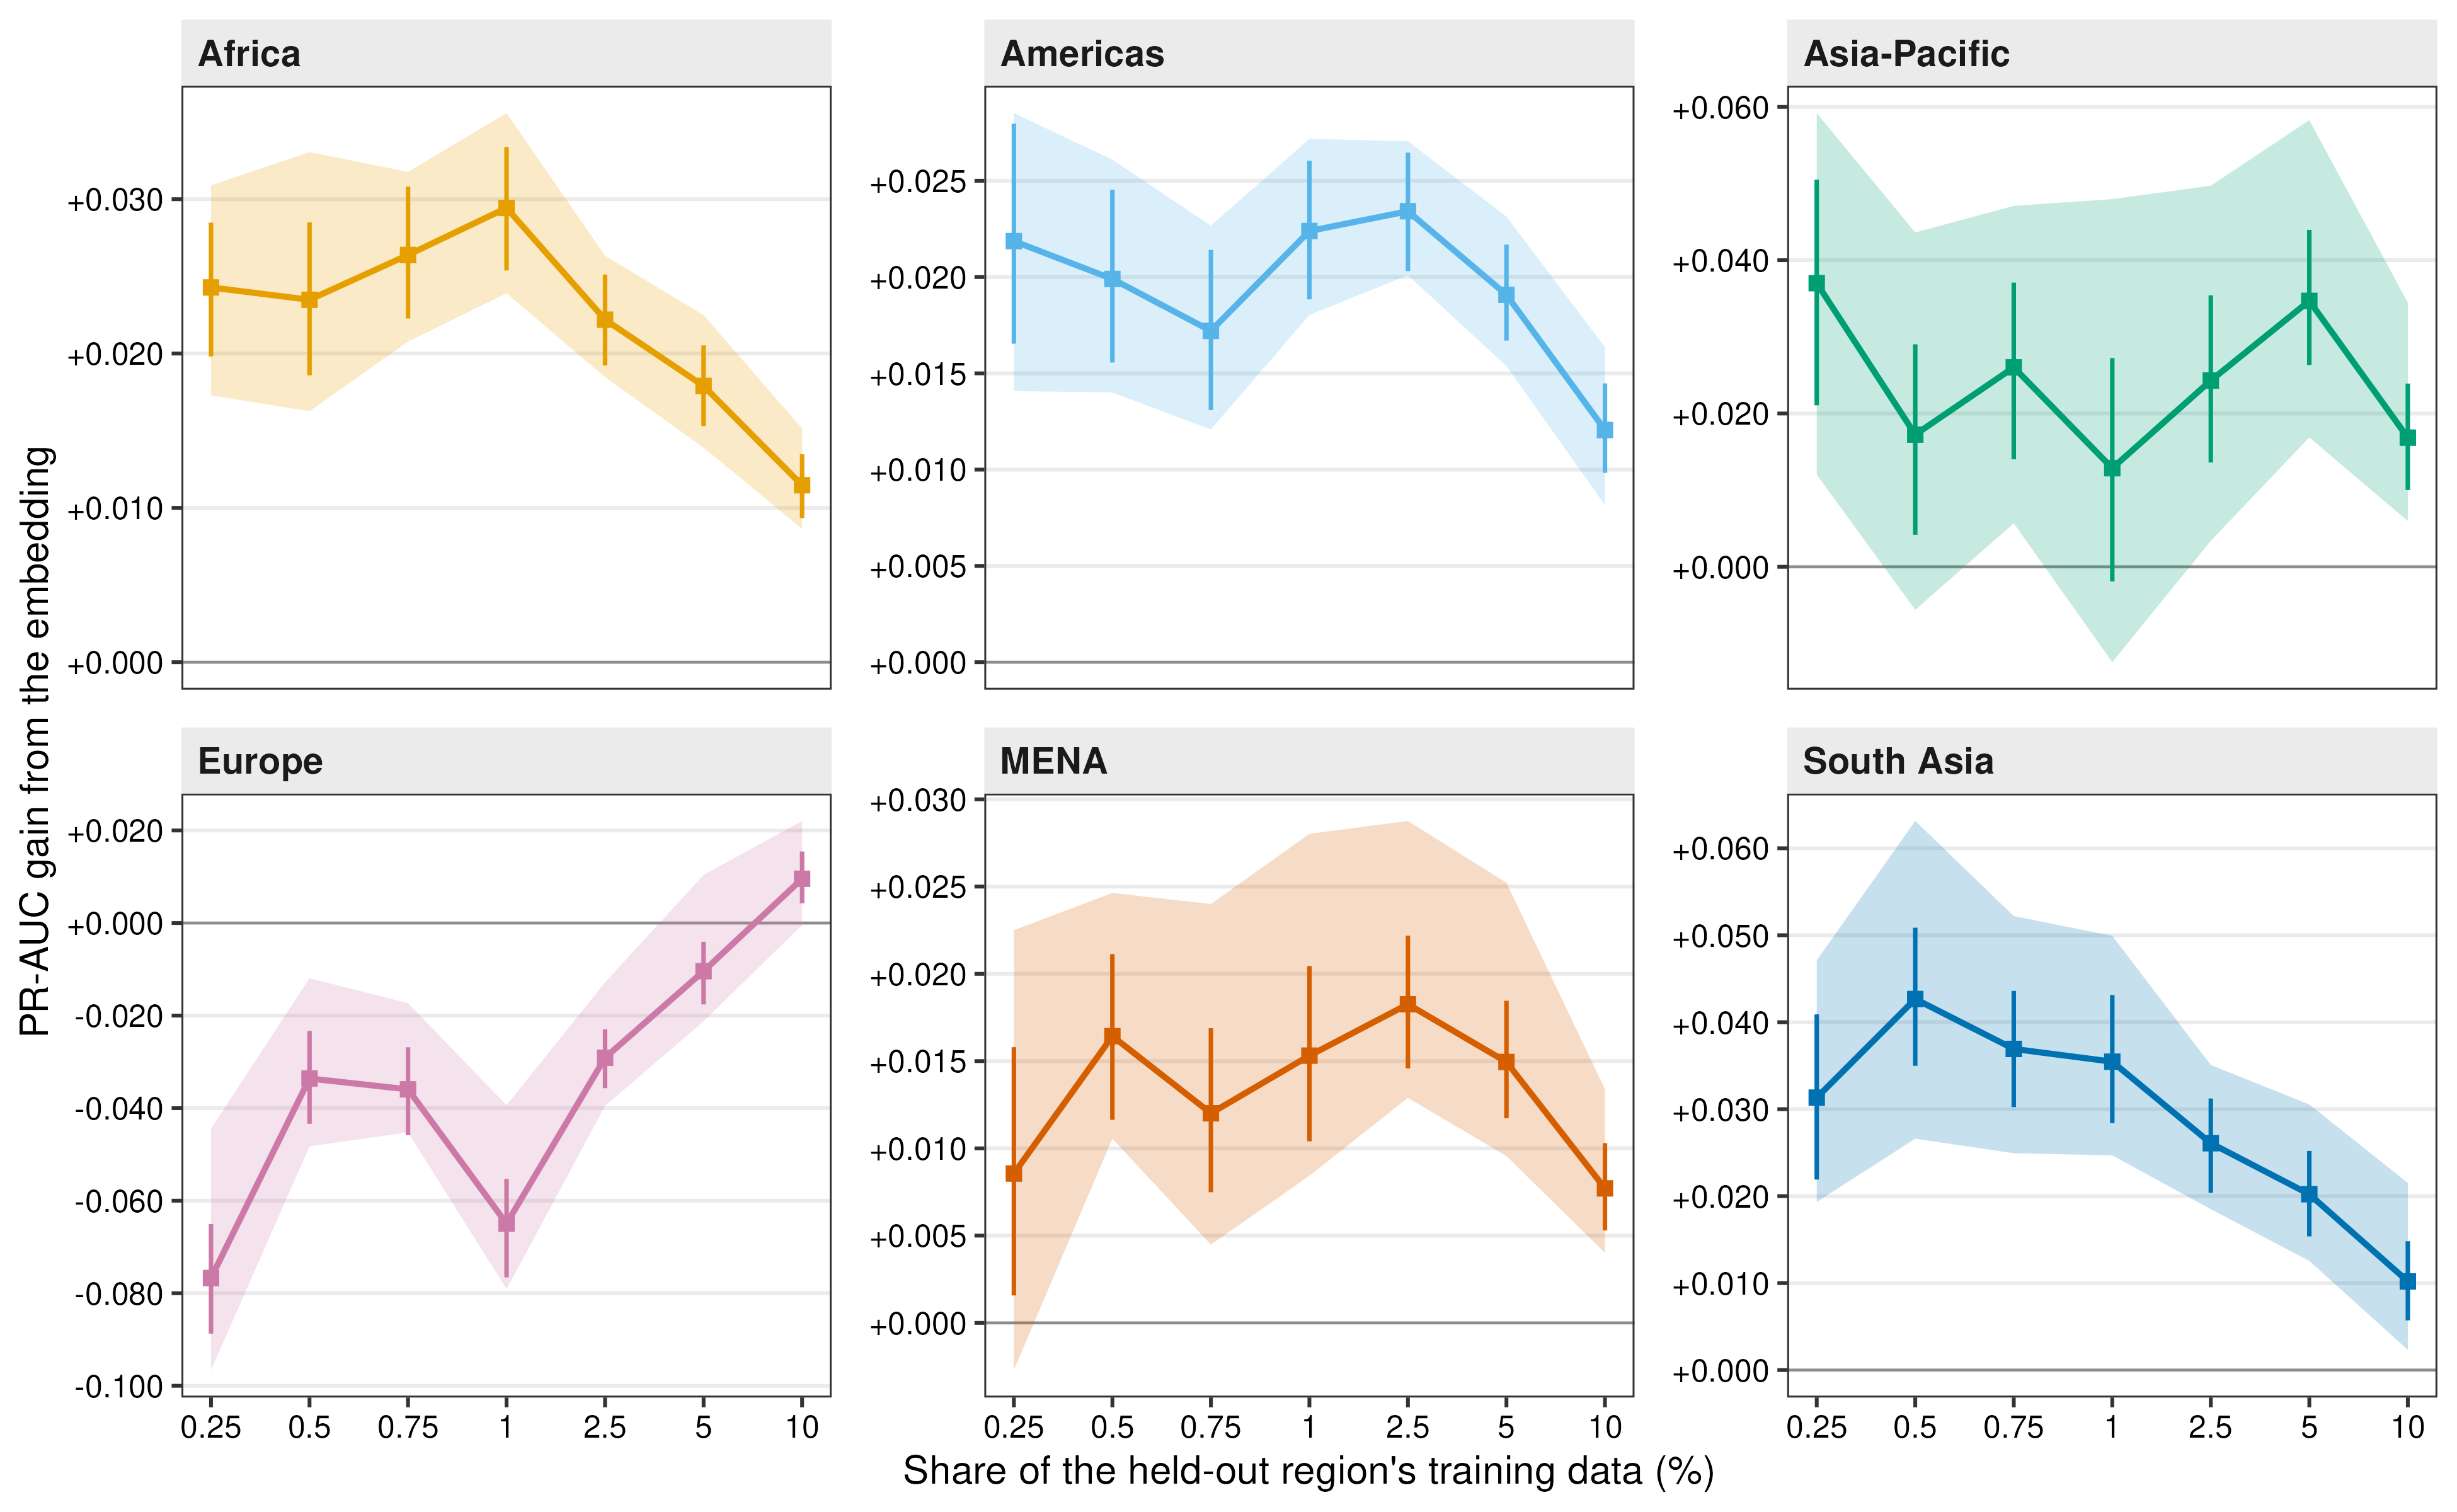
\includegraphics[width=\textwidth]{figures/fig_boot_share_regions_M.png}
\caption{Gain from the embedding by training share and held-out region. Band = 95\% spatial-block bootstrap interval; vertical lines = 95\% single-cell interval. Y-axes differ across panels.}
\label{fig:boot_share_regions}
\end{figure}
\begin{figure}[!htbp]
\centering
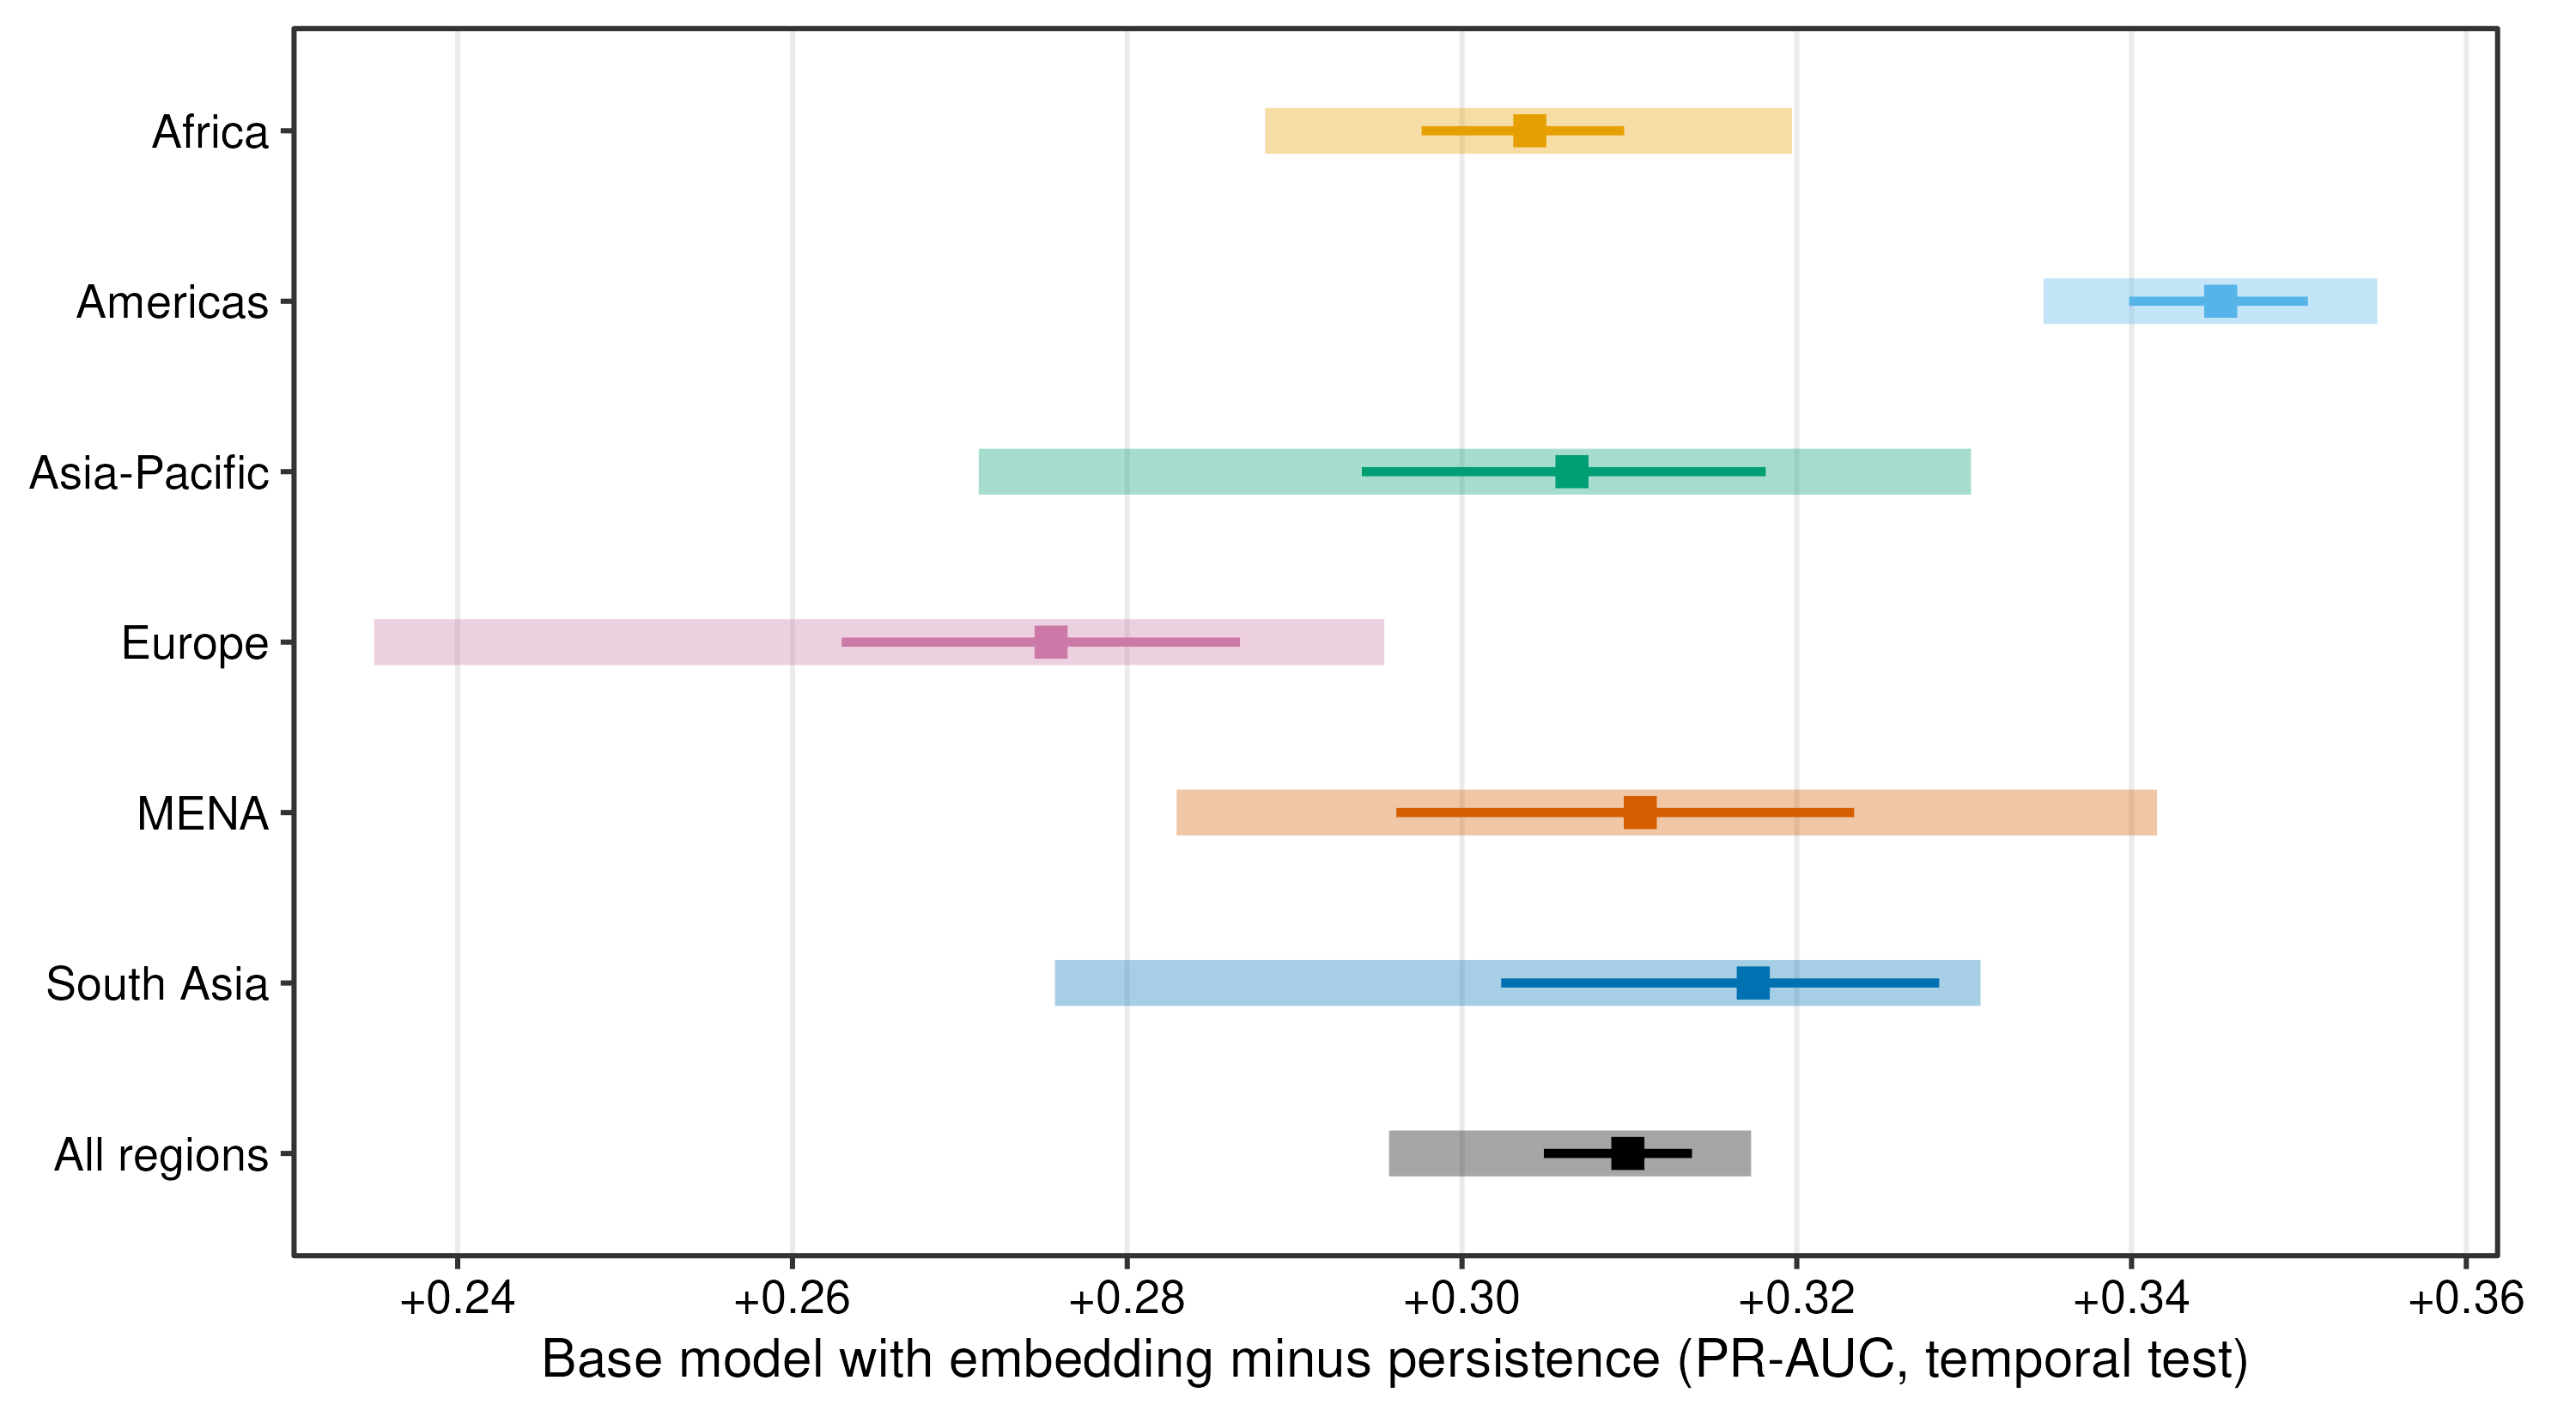
\includegraphics[width=0.85\textwidth]{figures/fig_boot_persistence_M.png}
\caption{Base model with the embedding minus persistence (violence in month $t$), by held-out region (temporal test, PR-AUC). Wide bars are 95\% spatial-block intervals; thin bars are single-cell intervals.}
\label{fig:boot_persistence}
\end{figure}

% CUT 2026-10-16 (superseded by Section~\ref{sec:civilian_case}): % moved from the main text 2026-10-11 (civilian scope check and AR-objective table)
% CUT 2026-10-16 (superseded by Section~\ref{sec:civilian_case}): \section{Civilian Targeting Scope Check}

% CUT 2026-10-16 (superseded by Section~\ref{sec:civilian_case}): %\subsection{Civilian-Deaths Target (Scope Check)}
% CUT 2026-10-16 (superseded by Section~\ref{sec:civilian_case}): \label{sec:civilian}
% CUT 2026-10-16 (superseded by Section~\ref{sec:civilian_case}): The results suggest that the transformer can be used for transfer learning in conflict forecasting, with the embedding adding information in most regions even when little local data are available. Here, I test the model on a narrower outcome, whether any violence against civilians occurs in a grid cell in the following month. This outcome is useful for two reasons. First, it is more specific and rarer than the general violence outcome, because violence against civilians is a subset of the violent events used above. This tests whether the embedding remains useful when violent cell-months are scarcer. Second, reducing violence against civilians in civil wars and other forms of political violence is a central goal of early-warning systems \citep{XX}. In turn, this example offers an intuitive frame of reference for the model. 

% CUT 2026-10-16 (superseded by Section~\ref{sec:civilian_case}): Table \ref{tab:civilian_scope} displays the results. 

% CUT 2026-10-16 (superseded by Section~\ref{sec:civilian_case}): \input{tables/table4_civilian_scope.tex}
% CUT 2026-10-16 (superseded by Section~\ref{sec:civilian_case}): % civilian = binarized etype_violence_against_civilians incidence, PR-AUC
% CUT 2026-10-16 (superseded by Section~\ref{sec:civilian_case}): % scored (Table~\ref{tab:civilian_scope}). Report honestly: transfer advantage
% CUT 2026-10-16 (superseded by Section~\ref{sec:civilian_case}): % and absolute performance both markedly weaker than general incidence, and
% CUT 2026-10-16 (superseded by Section~\ref{sec:civilian_case}): % Europe/Temporal is the one cell where emb\_base actually LOSES to base
% CUT 2026-10-16 (superseded by Section~\ref{sec:civilian_case}): % (-0.007). Do NOT frame as "mass atrocity" forecasting -- civilian incidence
% CUT 2026-10-16 (superseded by Section~\ref{sec:civilian_case}): % is a much lower bar than mass-atrocity scale (Valentino/Straus/Early Warning
% CUT 2026-10-16 (superseded by Section~\ref{sec:civilian_case}): % Project definitions -- citation still needed, see references.bib TODO).
% CUT 2026-10-16 (superseded by Section~\ref{sec:civilian_case}): % Keep general political-violence framing primary; this is a boundary/scope
% CUT 2026-10-16 (superseded by Section~\ref{sec:civilian_case}): % test -- consistent with what was sent to Babette Kania (USHMM) on the
% CUT 2026-10-16 (superseded by Section~\ref{sec:civilian_case}): % framing pivot.
\section{Forecasting Violence Against Civilians} % moved from the main text to the appendix 2026-10-16 (Jared) 

\label{sec:civilian_case}
% Possible alternative section names: "Forecasting Violence Against Civilians" or "Application to Civilian Targeting"
% NOTE: the appendix still holds the older "Civilian Targeting Scope Check" section (sec:civilian, table4_civilian_scope, s123 + original vocab). Delete or replace it once this section is written.

\subsection{Why Civilian Targeting}
% - Policy priority: protection of civilians is a core mandate in peacekeeping and atrocity prevention; ties to the USHMM early-warning agenda
% - Outcome: any violence-against-civilians event in a PRIO-GRID cell in the following month (ACLED event type)
% - Harder target than general incidence: rarer events, and civilian targeting follows its own strategic logic (cite XXX, e.g., Kalyvas 2006; Valentino 2014)
% - Question for this section: does the same pretrained encoder help forecast a narrower outcome it was never trained to predict?

% DRAFTED 2026-10-16 from the outline above
% NOTES 2026-10-21 (Claude): my draft prose removed (see Overleaf History); write this in your own words. Numbers are from the OLD encoders.
\begin{itemize}
\item What. Change the outcome to any violence against civilians in a cell in the following month.
\item Why. Protecting civilians is a core goal of peacekeeping, atrocity prevention and early warning (USHMM link). The outcome is narrower and rarer than general violence, and civilian targeting follows its own strategic logic \citep{kalyvas2006logic, valentino2014why}.
\item Question. Does the same embedding help forecast an outcome the encoder was not built for?
\end{itemize}

\subsection{Design}
% - Same 18 encoders as the main analysis (6 held-out regions x 3 seeds); no retraining for this outcome
% - Encoder stays frozen; only the gradient-boosted head is refit on the civilian target
% - Same LORO protocol, same temporal (train through 2020, test 2022 on) and pooled evaluations, same vocabulary remap
% - Comparison of interest is nested: base model plus embedding vs. base model alone (Table~\ref{tab:civilian_remap})

% DRAFTED 2026-10-16
% NOTES 2026-10-21 (Claude): my draft prose removed (see Overleaf History); write this in your own words. Numbers are from the OLD encoders.
\begin{itemize}
\item Same 18 encoders (six regions by three seeds), not retrained. Encoder frozen; only the gradient-boosted forecaster is refit on the civilian outcome.
\item Same protocol, evaluation periods and vocabulary remap. Comparison is nested (base plus embedding versus base).
\end{itemize}

\subsection{Results}
% - Embedding improves the base model in five of six regions in both evaluations
% - Average gain about +0.014 (temporal) and +0.009 (pooled), similar to or slightly larger than the general incidence result
% - Largest gains in Asia-Pacific (+0.037 temporal) and Africa (+0.019 temporal)
% - Europe is the exception: about zero in both modes, and the full model does not beat persistence there (hypothesis: very few civilian-targeting events in the test window; counts to be checked)
% - Translate a gain into XX more true positive cell-months and XX fewer false positives at a fixed threshold

% DRAFTED 2026-10-16
% NOTES 2026-10-21 (Claude): my draft prose removed (see Overleaf History); write this in your own words. Numbers are from the OLD encoders.
\begin{itemize}
\item Nested gain in five of six regions. Mean +0.016 (temporal); the pooled +0.011 goes to Section~\ref{app:pooled}. Largest in Asia-Pacific (+0.059) and Africa (+0.017).
\item Europe is the exception. No embedding gain, and no gain over persistence.
% CUT 2026-11-08 (needs a multi-day GPU rerun; Jared): \item Fine-tuned versus scratch (Table~\ref{tab:finetune_civilian}). +0.046 at 0.25 percent (Europe has no runs there), then close to zero and negative from 2.5 percent.
\end{itemize}
% PENDING: civilian fine-tuning (step 7b) results, jobs 56448906/56448907; alert counts for the civilian outcome (cell_alerts_agg.py civilian) not yet run.

\subsection{Implications for Early Warning}
% - Atrocity early-warning systems often cover places with little historical data; the encoder adds signal there without retraining region by region
% - The gains are modest, so the embedding complements rather than replaces hand-crafted risk models
% - Caveat: whether the gain comes from pretraining or from the encoder architecture is tested in the random-encoder control (Appendix Section XX)

% DRAFTED 2026-10-16
% NOTES 2026-10-21 (Claude): my draft prose removed (see Overleaf History); write this in your own words. Numbers are from the OLD encoders.
\begin{itemize}
\item Gains are modest, so the embedding complements rather than replaces existing risk models.
\item Why it still matters. Civilian-protection early warning often covers places with little recent data, and the encoder adds information there without retraining region by region.
\end{itemize}

% Source: outputs/eval_region_L_contrastive_e_loro_{region}_s{123,456,789}.csv, target civilian (Roar, Oct 14, 2026); all three seeds for every region.
\begin{table}[!htbp]
\centering
\caption{Embedding Gain for Forecasting Violence Against Civilians}
\label{tab:civilian_remap}
% UPDATED 2026-11-08 from figures_tables/tables_v5_20261108/tab_civilian_remap.tex (make_tables.py; eval_region_M_contrastive_e_fullsrc_loro_{region}_s{seed}.csv, target civilian)
\begin{tabular}{lccccc}
\hline
& \multicolumn{2}{c}{Temporal} & \multicolumn{2}{c}{Pooled} & Temporal \\
Region & Gain vs.\ base & Seeds $>0$ & Gain vs.\ base & Seeds $>0$ & Gain vs.\ persistence \\
\hline
Asia-Pacific & +0.059 & 3/3 & +0.012 & 3/3 & +0.166 \\
Africa & +0.017 & 3/3 & +0.011 & 3/3 & +0.197 \\
South Asia & +0.016 & 3/3 & +0.018 & 3/3 & +0.132 \\
Middle East and North Africa & +0.003 & 3/3 & +0.014 & 3/3 & +0.177 \\
Americas & +0.003 & 3/3 & +0.012 & 3/3 & +0.216 \\
Europe & $-$0.003 & 0/3 & $-$0.000 & 1/3 & +0.001 \\
\hline
Mean & +0.016 & & +0.011 & & +0.148 \\
\hline
\end{tabular}
\caption*{\footnotesize \textit{Note:} Outcome is any violence against civilians in a grid cell in the following month. Entries are PR-AUC differences averaged over three encoder seeds (123, 456, 789). ``Gain vs.\ base'' compares the gradient-boosted model with and without the frozen pretrained embedding; ``Gain vs.\ persistence'' compares the base plus embedding model with a persistence baseline. Temporal models train through 2020 and are tested on forecasts made from January 2022 onward; pooled results use five-fold cross-validation with cell-months assigned to folds at random, so they measure interpolation rather than forecasting.}
\end{table}

% Source: outputs/share_grid/metrics_finetune_{region}_s{seed}_f{share}_civ.csv (job 56448906); means over seeds 123/456/789 and five draws. Point estimates; bootstrap intervals pending (job 56448907).
% Europe 0.25 percent: no runs in the output (to check). Mean at 0.25 percent is over five regions.
% CUT 2026-11-08 (needs a multi-day GPU rerun; Jared): \begin{table}[!htbp]
% CUT 2026-11-08 (needs a multi-day GPU rerun; Jared): \centering
% CUT 2026-11-08 (needs a multi-day GPU rerun; Jared): \caption{Fine-Tuned Pretrained Encoder Versus the Same Network Trained From Scratch, Violence Against Civilians}
% CUT 2026-11-08 (needs a multi-day GPU rerun; Jared): \label{tab:finetune_civilian}
% CUT 2026-11-08 (needs a multi-day GPU rerun; Jared): \small
% CUT 2026-11-08 (needs a multi-day GPU rerun; Jared): \begin{tabular}{lccccccc}
% CUT 2026-11-08 (needs a multi-day GPU rerun; Jared): \hline
% CUT 2026-11-08 (needs a multi-day GPU rerun; Jared): & \multicolumn{7}{c}{Share of the held-out region's training data (\%)} \\
% CUT 2026-11-08 (needs a multi-day GPU rerun; Jared): Region & 0.25 & 0.5 & 0.75 & 1 & 2.5 & 5 & 10 \\
% CUT 2026-11-08 (needs a multi-day GPU rerun; Jared): \hline
% CUT 2026-11-08 (needs a multi-day GPU rerun; Jared): Africa & $-$0.011 & +0.026 & +0.008 & $-$0.009 & +0.014 & $-$0.011 & $-$0.006 \\
% CUT 2026-11-08 (needs a multi-day GPU rerun; Jared): Americas & +0.062 & +0.003 & +0.047 & $-$0.034 & $-$0.028 & $-$0.014 & $-$0.010 \\
% CUT 2026-11-08 (needs a multi-day GPU rerun; Jared): Asia-Pacific & +0.040 & +0.008 & +0.029 & +0.017 & $-$0.031 & $-$0.018 & $-$0.028 \\
% CUT 2026-11-08 (needs a multi-day GPU rerun; Jared): Europe & -- & +0.001 & $-$0.002 & $-$0.009 & +0.016 & $-$0.001 & $-$0.015 \\
% CUT 2026-11-08 (needs a multi-day GPU rerun; Jared): MENA & +0.107 & $-$0.015 & $-$0.023 & +0.032 & $-$0.019 & $-$0.024 & $-$0.030 \\
% CUT 2026-11-08 (needs a multi-day GPU rerun; Jared): South Asia & +0.030 & +0.040 & +0.011 & +0.003 & $-$0.013 & $-$0.038 & $-$0.012 \\
% CUT 2026-11-08 (needs a multi-day GPU rerun; Jared): \hline
% CUT 2026-11-08 (needs a multi-day GPU rerun; Jared): Mean & +0.046 & +0.010 & +0.012 & $-$0.000 & $-$0.010 & $-$0.018 & $-$0.017 \\
% CUT 2026-11-08 (needs a multi-day GPU rerun; Jared): Runs $>0$ (\%) & 68 & 62 & 53 & 53 & 40 & 24 & 23 \\
% CUT 2026-11-08 (needs a multi-day GPU rerun; Jared): \hline
% CUT 2026-11-08 (needs a multi-day GPU rerun; Jared): \end{tabular}
% CUT 2026-11-08 (needs a multi-day GPU rerun; Jared): \caption*{\footnotesize \textit{Note:} Outcome is any violence against civilians in a grid cell in the following month. Entries are PR-AUC differences, fine-tuned pretrained encoder minus the same network trained from scratch, averaged over three encoder seeds (123, 456, 789) and five draws of the training share. Both networks choose their learning rate and weight decay on 2021 validation data. Forecasts are made from January 2022 onward. The mean at 0.25 percent excludes Europe. The last row is the share of region, seed, and draw runs in which the pretrained encoder scores higher. Europe has no runs at 0.25 percent (--) because 0.25 percent of its 1,412 training-period positives is 4 cell-months, below the minimum of 5.}
% CUT 2026-11-08 (needs a multi-day GPU rerun; Jared): \end{table}

\clearpage
\section{Where the Embedding Changes Alerts}
\label{app:cell_alerts}

\subsection{Country-Level Alert Gains}
\label{app:country_alerts}

\begin{figure}[!htbp]
\centering
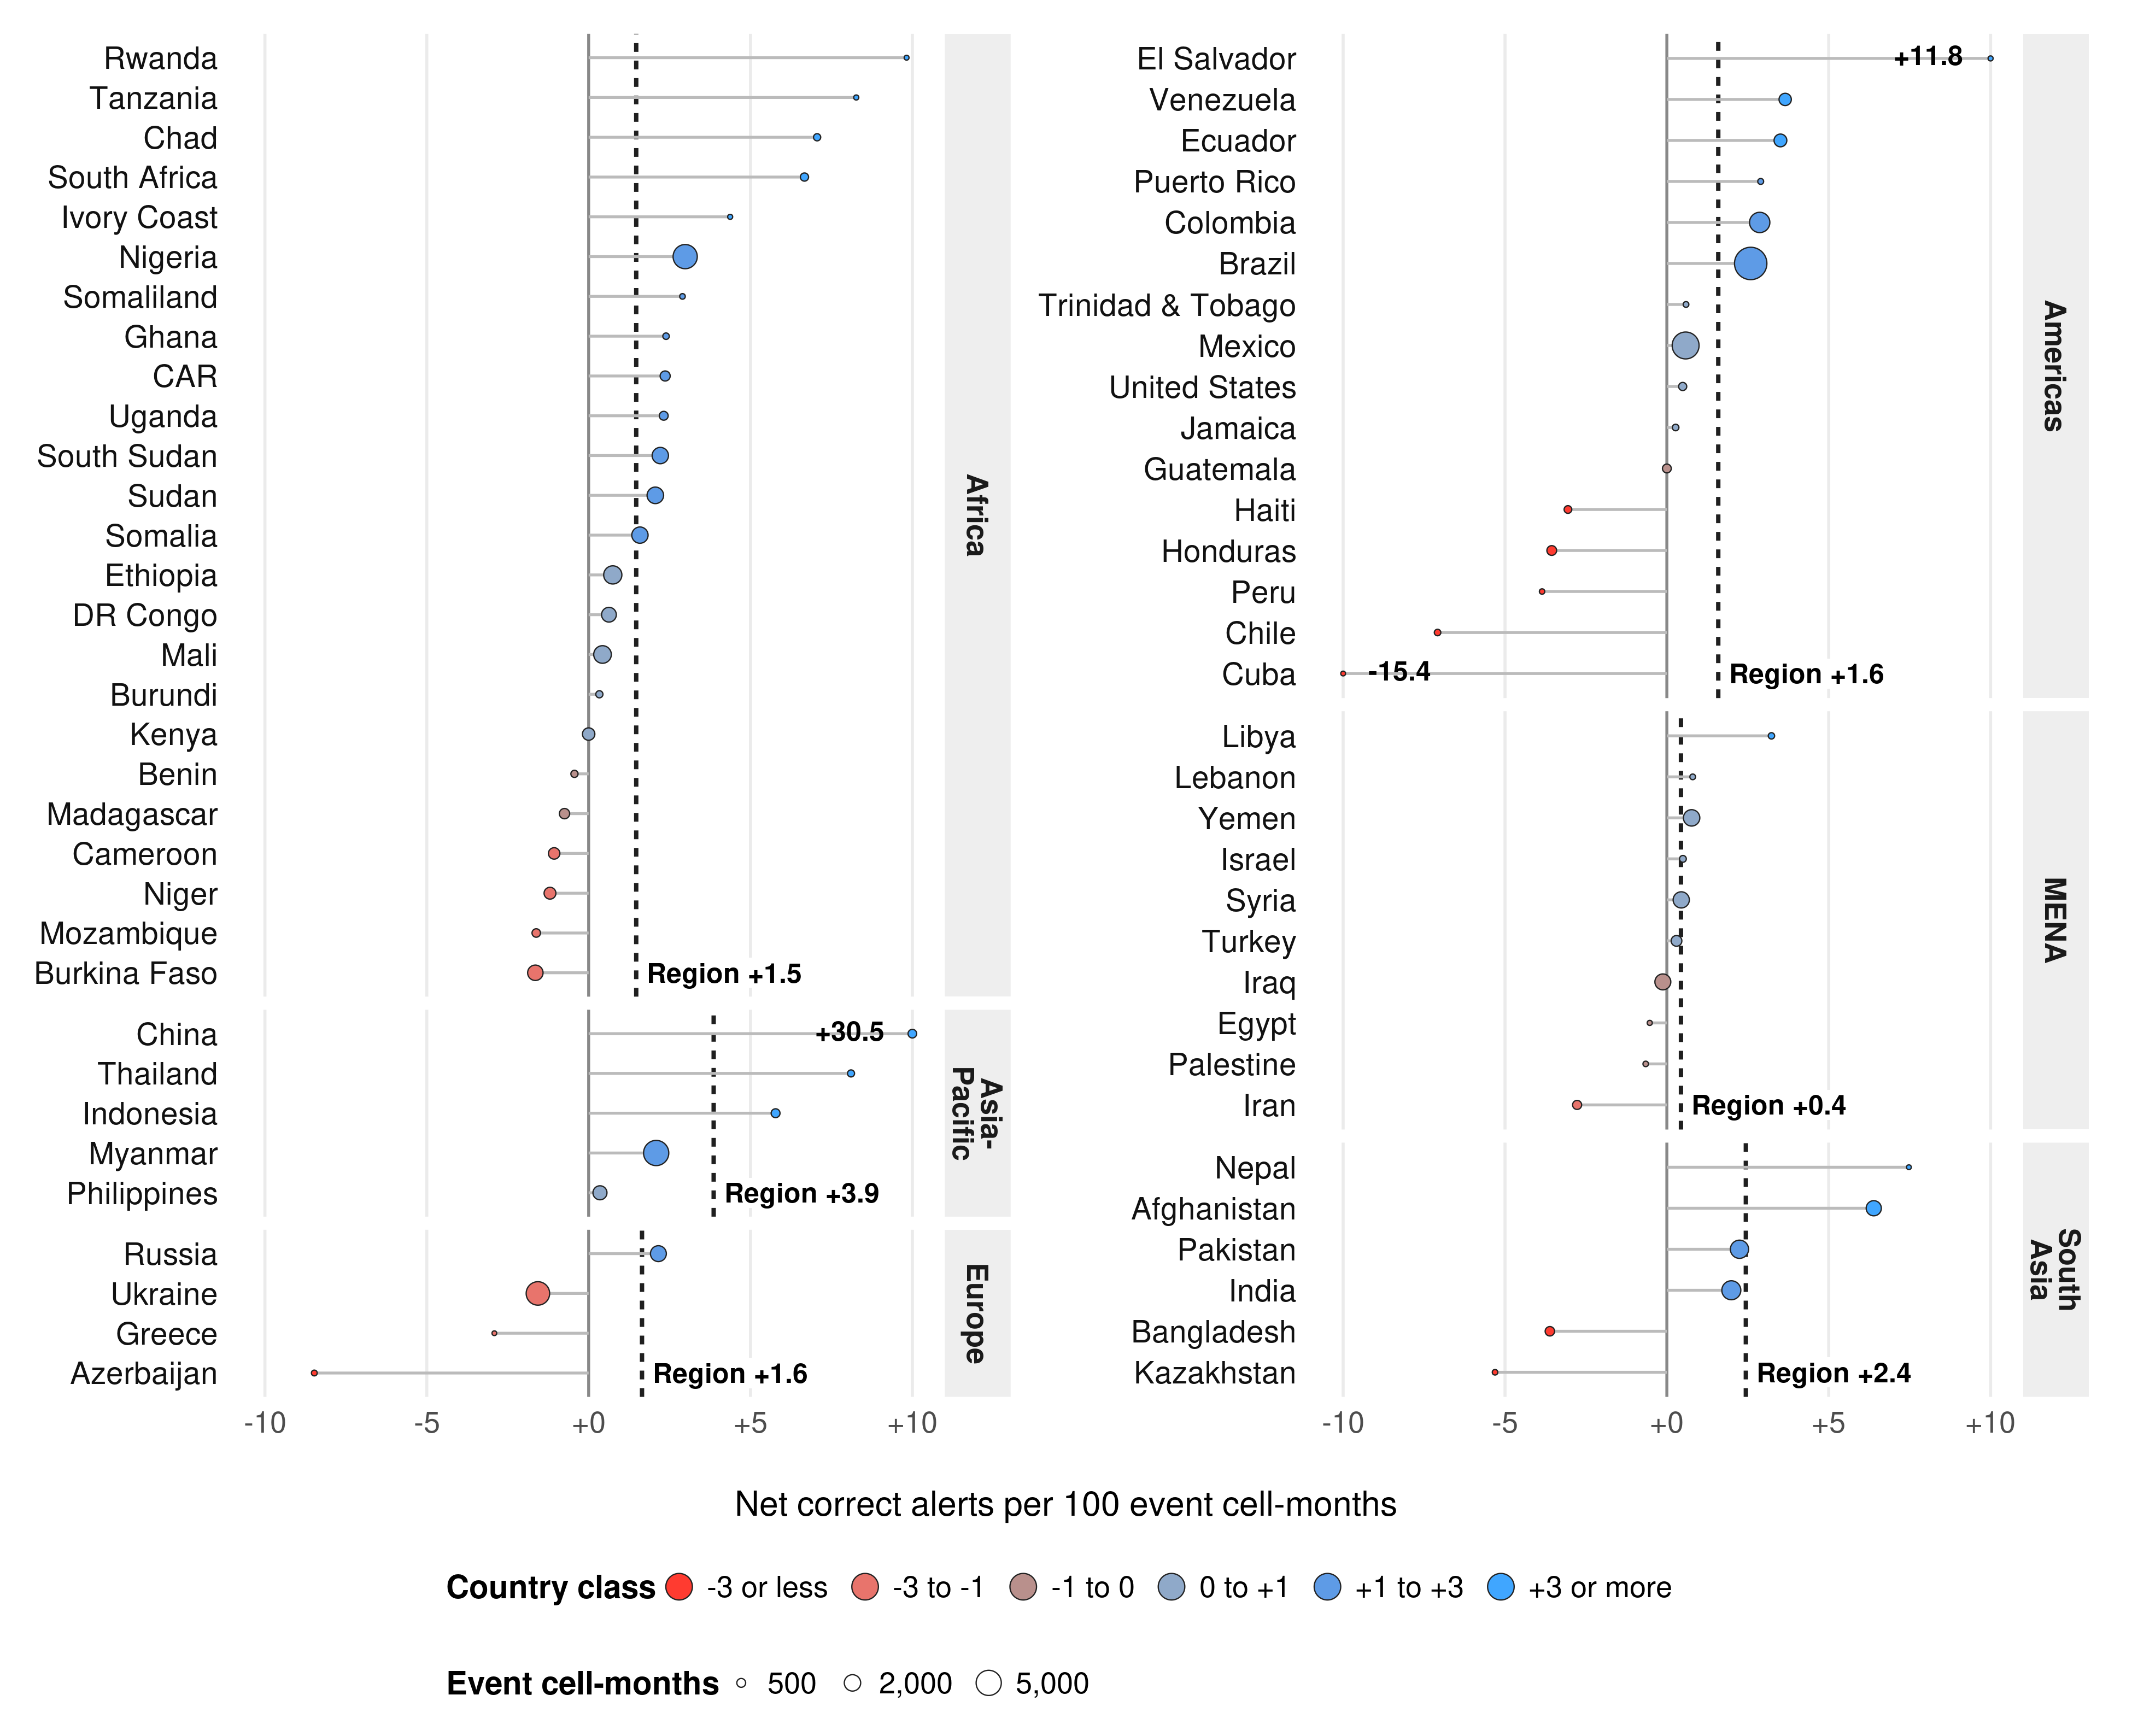
\includegraphics[width=\textwidth]{figures/fig_cell_alerts_countries_wide_M_fullsrc.png}
\caption{Net correct alerts per 100 event cell-months by country, base plus embedding against the base model at an equal alert budget, seed-averaged. Countries with at least 100 event cell-months, grouped by held-out region. Point size is the country's event cell-months; the dashed line is that region's mean.}
\label{fig:country_alerts}
\end{figure}

Of the 22 highest-exposure states, 19 see a net gain in true alarms, while Ukraine, Burkina Faso, and Iraq see a net loss. Across the 65 countries with at least 100 event cell-months, 44 gain and 21 lose.


The gains in forecasting are relatively small overall. Although the gains appear nominal, they are substantively meaningful. In particular, issuing the same number of alerts as the base model, the forecaster with the embedding correctly flags 710 more violent cell-months across the six regions, and therefore raises 710 fewer false alarms. The base plus embedding model's advantage over persistence is larger still. Issuing the same number of alerts as persistence, the base plus embedding model correctly flags 4,762 more violent cell-months across all regions (between 97 and 1,695 by region).\footnote{These counts rank all of a region's test cell-months together and set the number of alerts after the fact. They describe how well each model ranks cells, not a monthly alert rule an analyst could have applied in real time. Because both models issue the same number of alerts, each additional correct alert takes the place of a false alarm, so these gains do not come from issuing more alerts.} Matching the share of violent cell-months that persistence detects, it does so with 13,557 fewer false alarms across all regions (between 357 and 4,634 by region). Given that the transfer learning task is political violence, identifying 710 more violent cell-months could be consequential for both protecting human life and appropriately focusing resources in the most high-risk areas. Put differently, even if the gains are close to zero, they are consequential for the states and victims of these attacks.

% NOTES 2026-10-21 (Claude): my draft prose removed (see Overleaf History); write this in your own words. Numbers are from the OLD encoders.
% UPDATED 2026-10-29 (Claude): numbers below now from M full-source LORO (outputs/cell_alerts_{persistence,incidence}_M_fullsrc.csv.gz, seed-averaged over 123/456/789). Prior values were from the superseded encoders.
\begin{itemize}
\item What the map shows. For each cell, true alarms gained minus false alarms added by the base plus embedding model, with both models flagging the same number of cell-months.
\item Against persistence. 2,193 cells gain and 2,110 lose; net +4,762 true alarms.
\item Against the base model. Gains and losses sit side by side in the same conflict zones (1,452 cells gain, 1,293 lose); net +710.
\item Point to Figure~\ref{fig:country_alerts} for the by-country sums (label still missing, see bullets below).
\end{itemize}

% NOTES 2026-10-21 (Claude): my draft prose removed (see Overleaf History); write this in your own words. Numbers are from the OLD encoders.
\begin{itemize}
\item What. Score the same incidence-trained forecasts only on cell-months with no violence the month before (onset), and then only where neighbouring cells were also quiet.
\item Why. These are the cases where persistence cannot help, so they test whether the embedding adds information about new violence.
\item Numbers. Onset +0.017, positive in 18 of 18 runs. Quiet neighbours +0.009, 13 of 18. Best F1 +0.010, 18 of 18.
\end{itemize}

% Source: outputs/eval_region_L_contrastive_e_loro_{region}_s{seed}.csv, mode B_temporal, targets onset, noncontig_onset, rare_event_f1 (transfer_eval_region.py lines 214-227); means over seeds 123/456/789. Read 2026-10-17.
\begin{table}[!htbp]
\centering
\caption{Embedding Gain on Onsets and Rare Events (Temporal Test)}
\label{tab:onset_subsets}
\small
% UPDATED 2026-11-08 from figures_tables/tables_v5_20261108/tab_onset_subsets.tex (make_tables.py; eval_region_M_contrastive_e_fullsrc_loro_{region}_s{seed}.csv, B_temporal)
\begin{tabular}{lccccccccc}
\hline
& \multicolumn{3}{c}{Onset} & \multicolumn{3}{c}{Onset, quiet neighbours} & \multicolumn{2}{c}{Best F1} \\
Region & Share & Base & Gain & Share & Base & Gain & Base & Gain \\
\hline
Africa & 0.067 & 0.360 & +0.014 & 0.035 & 0.187 & +0.015 & 0.615 & +0.007 \\
Americas & 0.045 & 0.341 & +0.013 & 0.024 & 0.215 & +0.006 & 0.626 & +0.007 \\
Asia-Pacific & 0.023 & 0.292 & +0.034 & 0.010 & 0.118 & +0.022 & 0.654 & +0.021 \\
Europe & 0.020 & 0.173 & +0.028 & 0.013 & 0.085 & +0.001 & 0.630 & +0.012 \\
MENA & 0.038 & 0.370 & +0.007 & 0.017 & 0.142 & +0.015 & 0.744 & +0.003 \\
South Asia & 0.052 & 0.287 & +0.006 & 0.033 & 0.174 & $-$0.006 & 0.546 & +0.012 \\
\hline
Mean & 0.041 & 0.304 & +0.017 & 0.022 & 0.153 & +0.009 & 0.636 & +0.010 \\
Runs $>0$ & & & 18/18 & & & 13/18 & & 18/18 \\
\hline
\end{tabular}
\caption*{\footnotesize \textit{Note:} Onset columns score the incidence forecasts only on cell-months with no violent event in the month before the forecast month. Quiet-neighbour columns further require no violence in the cell's spatial lag in that month. Share is the share of those cell-months with violence the next month, which is also the PR-AUC of the lagged persistence forecast there. Base is the PR-AUC of the base model, and Gain is base plus embedding minus base. Best F1 is the highest F1 over thresholds on all test cell-months. Values are means over three encoder seeds.}
\end{table}

% ADDED 2026-10-20 by Claude: items to resolve in this section
\begin{itemize}
\item Figure~\ref{fig:country_alerts} is referenced above but no figure carries that label. Include figures/fig\_cell\_alerts\_countries\_final.png (or the 2row version) with \texttt{\textbackslash label\{fig:country\_alerts\}}.
\item Onset, quiet-neighbour, and best-F1 definitions appear only here. The main-text Discussion uses ``violence onset'' without a definition.
\end{itemize}

% CUT 2026-11-08 (needs a multi-day GPU rerun; Jared): \section{Autoregressive Pretraining Objective}
% CUT 2026-11-08 (needs a multi-day GPU rerun; Jared): \label{app:ar}


% CUT 2026-11-08 (needs a multi-day GPU rerun; Jared): \input{tables/table5_ar_baseline.tex}
% ADDED 2026-10-20 by Claude: items to resolve
% CUT 2026-11-08 (needs a multi-day GPU rerun; Jared): \begin{itemize}
% CUT 2026-11-08 (needs a multi-day GPU rerun; Jared): \item Discussion says the AR encoder is evaluated on 26 held-out countries in the pooled evaluation. The table does not mention the 26 countries or the pooled setup, and its source comment says 151 units. Reconcile and state both.
% CUT 2026-11-08 (needs a multi-day GPU rerun; Jared): \item Add the temporal setup alongside the pooled one (both setups, per plan).
% CUT 2026-11-08 (needs a multi-day GPU rerun; Jared): \item Define feature sets a, b, c, e, f in a table note; the tablenotes are commented out.
% CUT 2026-11-08 (needs a multi-day GPU rerun; Jared): \item List the 26 countries in Section~\ref{app:holdout_countries}.
% CUT 2026-11-08 (needs a multi-day GPU rerun; Jared): \end{itemize}
% Autoregressive-objective encoder: emb\_base advantage holds (15/15 positive,
% smaller magnitude, Table~\ref{tab:ar_baseline}) -- state as "not an artifact
% of the contrastive objective."
%
% STATUS AS OF 2026-09-29 (pulled directly from Roar this session):
%   AR-objective robustness check  — DONE, see Table~\ref{tab:ar_baseline}
%   Gradient-boosted base arm      — DONE, this IS the "base" arm throughout
%   Geography ablation             — NOT FOUND in outputs/ as of today; needs a run
%   Seeds 4-5                      — NOT FOUND (only s123/s456/s789 present); needs a run
%   Unseen-unit representation clarification — write up the resolution


% ===== APPENDIX SKELETONS added 2026-10-17 (Claude, at Jared's request). Headings/labels only; text and tables to be written by Jared. =====
\section{Event Fields}
\label{app:fields}
% TODO (Jared): one entry per field used by the encoder (event type, sub-event type, actor 1, actor 2, actor 1 type, actor 2 type, month offset); source: data_intermediate/vocab_super.json (vocabulary sizes) and ACLED codebook definitions.

% CUT 2026-11-08 (Jared, keep only the forecasting ensemble): \section{Models Without Static Covariates}
% CUT 2026-11-08 (Jared, keep only the forecasting ensemble): \label{app:nostatic}
% TODO (Jared): results without the 34 PRIO-GRID static covariates. NOTE: no such run found on Roar as of 2026-10-17 (geography ablation listed as NOT FOUND in the app:ar status notes); needs a run.

% CUT 2026-11-08 (needs a multi-day GPU rerun; Jared): \section{Countries Excluded From Pretraining}
% CUT 2026-11-08 (needs a multi-day GPU rerun; Jared): \label{app:holdout_countries}
% TODO (Jared): the 26 countries, their regions, and why they were held out.

% CUT 2026-11-08 (Jared, keep only the forecasting ensemble): \section{Encoder Design Selection}
% CUT 2026-11-08 (Jared, keep only the forecasting ensemble): \label{app:design}
% MOVED from main-text footnote 2026-10-20 (Claude)
% CUT 2026-11-08 (Jared, keep only the forecasting ensemble): The contrastive objective, encoder size, and feature set were chosen from a set of candidates scored on the same post-2021 test months, before the leave-one-region-out design.

% TODO (Jared): candidate objectives, encoder sizes and feature sets, with their scores on the post-2021 months. Table~\ref{tab:ar_baseline} (app:ar) covers the objective only.

% CUT 2026-11-08 (Jared, keep only the forecasting ensemble): \section{Transformers With Static Geographic Information}
% CUT 2026-11-08 (Jared, keep only the forecasting ensemble): \label{app:static_geo}
% TODO (Jared): comparison referenced in Appendix Section~\ref{app:cell_alerts} ("seen in Section ..."); no such section existed before 2026-10-17. Check whether this should point to app:nostatic instead.

% CUT 2026-11-08 (Jared, keep only the forecasting ensemble): \section{True and False Positives by Month}
% CUT 2026-11-08 (Jared, keep only the forecasting ensemble): \label{app:tpfp_month}
% TODO (Jared): monthly TP/FP for the nested comparison at equal alert counts; source outputs/cell_alerts_persistence.csv.gz and the incidence alert files.

\section{Forecasting Ensemble With a Four-Head Encoder}
\label{app:forecast_ensemble}
\label{app:ensemble} % ADDED 2026-10-20 by Claude: the Discussion cites app:ensemble
% ADDED 2026-10-20 by Claude: claims in the Discussion this section must support
\begin{itemize}
\item The embedding clearly improves forecasts of civilian victimization and violence onset.
\item It matches the XGBoost forecaster on overall violence.
\item It does not beat persistence for fatal violence (25 or more deaths).
\item Table of the four heads (incidence, civilian, onset, fatal25) for ens\_mean and ens\_stack against persistence and XGBoost, with the disclosure that encoder design was chosen on 2022+ months.
\end{itemize}
% TODO (Jared): forecasting with the pretrained encoding (not the LORO transfer design). Five all-region encoders (seeds 123, 456, 789, 101112, 131415) fine-tuned once each with four heads (incidence, civilian, onset, fatal25); train 1990-2020, stop 2021-01..06, stack 2021-07..12, test 2022-01 on; combiners ens_mean and ens_stack vs persistence and XGBoost. Results: outputs/ens/scores_mt_{target}.csv (jobs 56515866-71, running 2026-10-17). Disclose that encoder design was chosen on 2022+ months.



\section{Pooled (Interpolation) Evaluation}
\label{app:pooled}
% ADDED 2026-10-20 by Claude: all pooled results live here; the main text reports only the temporal design (train through 2020, early stopping on 2021, forecasts from January 2022).
\begin{itemize}
\item Define the pooled design. Five-fold cross-validation with cell-months assigned to folds at random, so it measures interpolation rather than forecasting or transfer over time.
\item Pooled version of Figure~\ref{fig:loro_gains} (persistence, base, base plus embedding by held-out region). The Mode A pooled rows are in the same source CSVs as the temporal rows.
\item Pretrained versus random encoder, pooled (Table~\ref{tab:random_pooled}). The gap is +0.001 (positive in 15 of 18 runs). State plainly that the pretraining advantage appears in the temporal test, not in the pooled one.
% CUT 2026-11-08 (needs a multi-day GPU rerun; Jared): \item Autoregressive objective (Section~\ref{app:ar}). The 15 feature-set and seed combinations cited in the Discussion are pooled results on the 26 held-out countries; add the temporal counterpart.
\item Civilian outcome pooled column (Table~\ref{tab:civilian_remap}).
\end{itemize}

\section{Smaller and Medium Encoders}
\label{app:sizes}
% MOVED from main-text footnote 2026-10-20 (Claude)
I replicate the main results using two other transformers that use the same (a) input data, (b) training, validation, and testing sets, and (c) contrastive pretraining objective and early stopping rule. The models differ in embedding width, number of layers, number of attention heads, and learning rate. The first model is a smaller encoder with a 64-dimensional embedding, 2 layers, 4 attention heads, and a learning rate of $10^{-3}$. The second model is a medium encoder with a 128-dimensional embedding, 4 layers, 8 attention heads, and a learning rate of $5 \times 10^{-4}$.

% ADDED 2026-10-20 by Claude
\begin{itemize}
\item Promised in the Protocols footnote (formerly ``Appendix Section XX'').
\item Repeat Figure~\ref{fig:loro_gains} and the fine-tuning comparison with the small ($d=64$, 2 layers, 4 heads, learning rate $10^{-3}$) and medium ($d=128$, 4 layers, 8 heads, $5\times10^{-4}$) encoders, 18 LORO encoders each.
\item State the decision rule for not training the extra-large encoder.
\item Fixed 30-epoch cap (patience 15 often did not trigger) \citep{prechelt1998early, goodfellow2016deep}.
\end{itemize}

% ADDED 2026-10-28 by Claude: encoder-size ladder skeleton (S/M/L). Frozen-embedding numbers from outputs/bootstrap_ci_{S,M,L}_fullsrc_block5.csv and the matching _rand.csv files.
\subsection{Frozen Embedding Results by Encoder Size}
\label{app:sizes_frozen}
Table~\ref{tab:sizes_frozen} reports the frozen-embedding step of the ladder for the small, medium and large encoders.

\begin{table}[!htbp]
\centering\footnotesize
\caption{Frozen embedding by encoder size (temporal test, PR-AUC differences, all regions)}
\label{tab:sizes_frozen}
\begin{tabular}{lccc}
\hline
Comparison & Small (S) & Medium (M) & Large (L) \\
\hline
Base + emb. $-$ persistence & $+0.3058$ & $+0.3099$ & $+0.3095$ \\
 & [$+0.2918$, $+0.3137$] & [$+0.2956$, $+0.3173$] & [$+0.2954$, $+0.3170$] \\
Base + emb. $-$ base & $+0.0085$ & $+0.0126$ & $+0.0122$ \\
 & [$+0.0052$, $+0.0115$] & [$+0.0094$, $+0.0153$] & [$+0.0082$, $+0.0152$] \\
Pretrained $-$ random encoder & $+0.0057$ & $+0.0045$ & $+0.0061$ \\
 & [$+0.0031$, $+0.0075$] & [$+0.0024$, $+0.0066$] & [$+0.0044$, $+0.0080$] \\
\hline
\end{tabular}
\begin{minipage}{0.98\textwidth}\footnotesize\vspace{0.5ex}
Notes. Equal-weight mean of the six held-out regions, averaged over three encoder seeds (123, 456, 789). Brackets are 95\% intervals from 1,000 paired bootstrap replicates resampling $5^\circ \times 5^\circ$ blocks of grid cells. M is the main-text encoder; for M the gain over persistence is positive in all six regions and the gain over the base model is positive in 18 of 18 region-seed runs. Built from outputs/bootstrap\_ci\_\{S,M,L\}\_fullsrc\_block5.csv and the matching \_rand.csv files.
\end{minipage}
\end{table}

\subsection{Fine-Tuning by Encoder Size}
\label{app:sizes_finetune}
% FILLED 2026-10-29 by Claude from outputs/bootstrap_ft_fullsrc_{S,M,L}_top2_block5.csv (ALL rows, equal-weight mean of the six held-out regions).
Table~\ref{tab:sizes_finetune_full} reports the fine-tuning step of the ladder for the three encoder sizes, with all parameters tuned, and Table~\ref{tab:sizes_finetune} repeats it with only the top two layers tuned.

% ADDED 2026-10-31 by Claude from outputs/bootstrap_ft_fullsrc_{S,M,L}_full_block5.csv (ALL rows, equal-weight mean of the six held-out regions, B 1000).
\begin{table}[!htbp]
\centering\scriptsize\setlength{\tabcolsep}{2.5pt}
\caption{Fine-tuning by encoder size, all parameters tuned (temporal test, PR-AUC difference over the same network trained from scratch, all regions)}
\label{tab:sizes_finetune_full}
\resizebox{\textwidth}{!}{\begin{tabular}{lccccccc}
\hline
 & \multicolumn{7}{c}{Share of the held-out region's training data} \\
Encoder & 0.25\% & 0.5\% & 0.75\% & 1\% & 2.5\% & 5\% & 10\% \\
\hline
Small (S) & $+0.062$ & $+0.028$ & $+0.022$ & $+0.005$ & $+0.001$ & $+0.007$ & $+0.002$ \\
 & [$+0.047$, $+0.074$] & [$+0.020$, $+0.039$] & [$+0.015$, $+0.030$] & [$-0.000$, $+0.013$] & [$-0.003$, $+0.008$] & [$+0.004$, $+0.013$] & [$-0.001$, $+0.006$] \\[2pt]
Medium (M) & $+0.053$ & $+0.014$ & $+0.025$ & $+0.014$ & $-0.007$ & $-0.018$ & $-0.010$ \\
 & [$+0.038$, $+0.063$] & [$+0.007$, $+0.021$] & [$+0.018$, $+0.031$] & [$+0.008$, $+0.020$] & [$-0.011$, $-0.003$] & [$-0.022$, $-0.012$] & [$-0.012$, $-0.007$] \\[2pt]
Large (L) & $+0.056$ & $+0.022$ & $+0.028$ & $+0.008$ & $-0.005$ & $+0.005$ & $-0.001$ \\
 & [$+0.041$, $+0.066$] & [$+0.015$, $+0.029$] & [$+0.019$, $+0.036$] & [$+0.003$, $+0.014$] & [$-0.008$, $+0.001$] & [$+0.000$, $+0.010$] & [$-0.005$, $+0.002$] \\
\hline
\end{tabular}}
\begin{minipage}{0.98\textwidth}\footnotesize\vspace{0.5ex}
Notes. Equal-weight mean of the six held-out regions, averaged over three encoder seeds and five draws of the training share. Brackets are 95\% intervals from 1,000 paired bootstrap replicates resampling $5^\circ \times 5^\circ$ blocks of grid cells. All parameters of the encoder and the output layer are tuned.
\end{minipage}
\end{table}

\begin{table}[!htbp]
\centering\scriptsize\setlength{\tabcolsep}{2.5pt}
\caption{Fine-tuning by encoder size, top two layers tuned (temporal test, PR-AUC difference over the same network trained from scratch, all regions)}
\label{tab:sizes_finetune}
\resizebox{\textwidth}{!}{\begin{tabular}{lccccccc}
\hline
& \multicolumn{7}{c}{Share of the held-out region's training data} \\
Encoder & 0.25\% & 0.5\% & 0.75\% & 1\% & 2.5\% & 5\% & 10\% \\
\hline
Small (S) & $+0.051$ & $+0.005$ & $+0.017$ & $-0.013$ & $-0.011$ & $+0.000$ & $-0.001$ \\
& [$+0.033$, $+0.067$] & [$-0.004$, $+0.018$] & [$+0.007$, $+0.028$] & [$-0.021$, $-0.002$] & [$-0.016$, $-0.004$] & [$-0.004$, $+0.006$] & [$-0.006$, $+0.004$] \\[2pt]
Medium (M) & $+0.037$ & $+0.004$ & $+0.009$ & $+0.005$ & $-0.023$ & $-0.022$ & $-0.014$ \\
& [$+0.021$, $+0.049$] & [$-0.006$, $+0.013$] & [$-0.003$, $+0.017$] & [$-0.005$, $+0.012$] & [$-0.030$, $-0.017$] & [$-0.027$, $-0.017$] & [$-0.019$, $-0.010$] \\[2pt]
Large (L) & $+0.024$ & $-0.002$ & $-0.002$ & $-0.011$ & $-0.030$ & $-0.037$ & $-0.024$ \\
& [$+0.007$, $+0.039$] & [$-0.013$, $+0.010$] & [$-0.013$, $+0.011$] & [$-0.021$, $-0.002$] & [$-0.037$, $-0.023$] & [$-0.044$, $-0.031$] & [$-0.030$, $-0.019$] \\
\hline
\end{tabular}}
\begin{minipage}{0.98\textwidth}\footnotesize\vspace{0.5ex}
Notes. Equal-weight mean of the six held-out regions, averaged over three encoder seeds and five draws of the training share. Brackets are 95\% intervals from 1,000 paired bootstrap replicates resampling $5^\circ \times 5^\circ$ blocks of grid cells. Only the top two transformer layers and the output layer are tuned.
\end{minipage}
\end{table}

% BULLET NOTES 2026-10-29 by Claude, for Jared to write prose from. Delete this block once the prose is written.
\begin{itemize}
\item What. The fine-tuning rung of the ladder for all three sizes, all parameters tuned, against the same architecture trained from scratch (Table~\ref{tab:sizes_finetune_full}). Table~\ref{tab:sizes_finetune} reports the top-two-layer arm.
\item Common pattern. Every size is positive with an interval that excludes zero at 0.25, 0.5 and 0.75 percent. At 0.25 percent the gains are S +0.062, M +0.053 and L +0.056, with overlapping intervals.
\item At 1 percent. M (+0.014) and L (+0.008) exclude zero, and S (+0.005 [$-$0.000, +0.013]) does not.
\item With more data. M is negative from 2.5 percent on ($-$0.007, $-$0.018, $-$0.010), each interval excluding zero. S and L stay near zero, and both are positive at 5 percent (S +0.007 [+0.004, +0.013], L +0.005 [+0.000, +0.010]). The decline at larger shares is clearest for M.
\end{itemize}

\subsection{Brazil Cross-Domain Transfer by Encoder Size}
\label{app:sizes_brazil}
% FILLED 2026-10-29 by Claude. S from outputs/crossdomain/xd_s_boot.csv (rungs C0_S and C1_S); M and L from outputs/crossdomain/xd_m_boot.csv (rungs C0_M, C1_M, C0_L and C1_L). All rows status complete, so no size is missing.
Table~\ref{tab:sizes_brazil} repeats the Brazil homicide comparisons of Section~\ref{sec:brazil} for the three encoder sizes.

\begin{table}[!htbp]
\centering\footnotesize
\caption{Brazil homicides by encoder size (relative reduction in Poisson deviance, \%)}
\label{tab:sizes_brazil}
\begin{tabular}{lccc}
\hline
Comparison & Small (S) & Medium (M) & Large (L) \\
\hline
Pretrained vs.\ random encoder, 0.25\% & $+7.6$ & $+11.1$ & $+16.5$ \\
& [$+3.7$, $+11.1$] & [$+6.2$, $+16.7$] & [$+10.6$, $+23.7$] \\
Pretrained vs.\ random encoder, 1\% & $+5.6$ & $+5.7$ & $+6.1$ \\
& [$+4.4$, $+6.8$] & [$+4.2$, $+7.6$] & [$+3.9$, $+9.4$] \\
Pretrained vs.\ random encoder, all data & $+4.1$ & $+2.8$ & $+1.9$ \\
& [$+3.4$, $+4.9$] & [$+2.0$, $+3.4$] & [$+1.4$, $+2.4$] \\
Pretrained vs.\ base, 1\% & $+6.4$ & $+6.8$ & $+6.6$ \\
& [$+5.2$, $+7.4$] & [$+5.8$, $+7.8$] & [$+5.3$, $+7.6$] \\
\hline
Pre-registered fine-tuning test, 1\% & $+5.4$ & $+3.6$ & $+5.7$ \\
& [$-1.6$, $+11.3$] & [$-0.4$, $+7.0$] & [$+0.2$, $+11.3$] \\
\hline
\end{tabular}
\begin{minipage}{0.92\textwidth}\footnotesize\vspace{0.5ex}
Notes. Positive values favor the first model named. Means over three encoder seeds (123, 456, 789) and five draws of the training share, one draw with all data. The frozen-embedding rows above the line carry 95\% paired bootstrap intervals that resample test cells and seed-draw pairs, as in Table~\ref{tab:brazil}. The pre-registered fine-tuning test compares the encoder with its top two layers and output layer tuned against the same network trained from scratch, and carries the cell bootstrap interval used for the pre-registered rule in Section~\ref{sec:brazil}. Each encoder is the size-matched encoder pretrained without the Americas.
\end{minipage}
\end{table}

% BULLET NOTES 2026-10-29 by Claude, for Jared to write prose from. Delete this block once the prose is written.
\begin{itemize}
\item What. The Brazil cross-domain test repeated at all three sizes. Every cell is a completed run, nothing is pending.
\item Scarce data favor the big encoder. Against the random encoder at 0.25 percent the gap widens with size, S $+7.6$, M $+11.1$, L $+16.5$, and every interval excludes zero.
\item With all the data the ordering flips, S $+4.1$, M $+2.8$, L $+1.9$. The advantage of pretraining shrinks as local data grow, fastest for the largest encoder.
\item Against the base model at 1 percent the three sizes are indistinguishable, $+6.4$, $+6.8$ and $+6.6$.
\item Pre-registered comparison (top two layers tuned versus scratch, 1 percent). S +5.4 percent [$-$1.6, +11.3], M +3.6 [$-$0.4, +7.0], L +5.7 [+0.2, +11.3]. Point estimates are similar across sizes, and the intervals overlap. Appendix Section~\ref{app:brazil_prereg} reports this comparison on its own.
\item Note for the size discussion. In Brazil the gain over the random encoder at 0.25 percent is largest for L (+16.5 vs +11.1 for M), though the intervals overlap.
\end{itemize}

\subsection{Pre-Registered Fine-Tuning Test for Brazil}
\label{app:brazil_prereg}
% MOVED 2026-10-29 by Claude from Section~\ref{sec:brazil} at Jared's request. Effect and intervals from outputs/crossdomain/xd_m_boot.csv (rungs C0_M and C0_L) and xd_s_boot.csv (rung C0_S), comparison scratch versus top2, cell bootstrap.
Before running the cross-domain test I registered a single comparison, the encoder fine-tuned on 1 percent of Brazil's data with its top two layers and output layer tuned, against the same network trained from scratch, with a 2 percent threshold set in advance.

\begin{itemize}
\item Effect. With the M encoder the fine-tuned model reduces Poisson deviance by 3.6 percent relative to the scratch network, cell-bootstrap interval [$-$0.4, +7.0].
\item Other sizes. S gives +5.4\% [$-$1.6, +11.3] and L gives +5.7\% [+0.2, +11.3] on the same comparison (Table~\ref{tab:sizes_brazil}).
\item Precision. With three encoder seeds and five draws of the training share, the interval spans about 7 percentage points, wider than the 2 percent threshold, so the comparison cannot distinguish an effect of that size from zero.
\item Architecture note. For M the top two layers are half the network, two of four, so the tuned and frozen arms are less distinct than the label suggests.
\end{itemize}

\section{Fine-Tuning Details}
\label{app:ft_details}
% ADDED 2026-10-20 by Claude
\begin{itemize}
\item The main text says both networks search ``the same grid of learning rates and weight decays'' without listing it. Give the grid (learning rates $3\times10^{-5}$, $10^{-4}$, $3\times10^{-4}$, $10^{-3}$; weight decay 0 or 0.01), maximum epochs (50), patience (5), the linear output layer on the summary token, and the class-weighted loss.
\item State the 2021 validation draw at the same share and the minimum number of positives. The civilian table note says a minimum of 5; the code floor is 10 validation positives. Reconcile.
\item State how the five stratified draws are seeded.
\end{itemize}

\section{Data Sources, Coverage, and Event-Type Harmonization}
\label{app:harmonize}
% MOVED from main-text footnote 2026-10-20 (Claude)
When a cell-month has more than 200 events, I keep the 200 most recent. I combine the two sources without removing events that appear in both. About 30 percent of the grid-cell days with a UCDP event also have an ACLED event, so event counts and sequences include some duplicates, although the binary outcome is unaffected. UCDP coverage ends in December 2024, so outcomes in 2025 come from ACLED alone. Events recorded only by UCDP account for 4.3 percent of violent cell-months in the test period.

% ADDED 2026-10-20 by Claude
\begin{itemize}
\item The Introduction says event types are harmonized across ACLED and UCDP. Give the mapping from UCDP violence types to ACLED event and sub-event types.
\item ACLED coverage start year by region (training rows from 1990 rely on UCDP alone where ACLED begins later), UCDP end date (December 2024), and the overlap and UCDP-only shares reported in the Data footnote.
\end{itemize}

\section{Baseline Features}
\label{app:features}
% ADDED 2026-10-20 by Claude
\begin{itemize}
\item Define each baseline feature used by the base model (violence lags 1, 3, 6; spatial lag as the mean of the four neighbouring cells at $t-1$; rolling violent and all-event counts; any event and log event density at $t-1$; months since the last event; the 34 PRIO-GRID covariates with their sources).
\item State the information set (sequences and lags stop at $t-1$; months since last event and persistence use month $t$).
\end{itemize}


% CUT 2026-11-08 (Jared, keep only the forecasting ensemble): \section{Applying the Conflict Encoder to Other Domains}
% CUT 2026-11-08 (Jared, keep only the forecasting ensemble): \label{app:cross_domain}
% ADDED 2026-10-20 by Claude
% CUT 2026-11-08 (Jared, keep only the forecasting ensemble): \begin{itemize}
% CUT 2026-11-08 (Jared, keep only the forecasting ensemble): \item Promised in the Discussion (fourth limitation): the conflict encoder, without further pretraining, applied to crime and dengue does not improve forecasting.
% CUT 2026-11-08 (Jared, keep only the forecasting ensemble): \item Describe how crime and dengue records are mapped into the conflict encoder's fields, the units, target, and shares.
% CUT 2026-11-08 (Jared, keep only the forecasting ensemble): \item Report both arms (frozen embedding in the gradient-boosted forecaster; fine-tuned vs.\ scratch) by share.
% CUT 2026-11-08 (Jared, keep only the forecasting ensemble): \end{itemize}

% CUT 2026-11-05 (to-do notes; nothing cites app:domain_alerts): \section{Alert Counts for Turnout, Crime, and Dengue}
% CUT 2026-11-05 (to-do notes; nothing cites app:domain_alerts): \label{app:domain_alerts}
% CUT 2026-11-05 (to-do notes; nothing cites app:domain_alerts): % ADDED 2026-10-20 by Claude
% CUT 2026-11-05 (to-do notes; nothing cites app:domain_alerts): \begin{itemize}
% CUT 2026-11-05 (to-do notes; nothing cites app:domain_alerts): \item The Discussion reports 1,204, 3,799, and 121 more true alarms at 0.25 percent. Table~\ref{tab:domains} reports only PR-AUC differences. Add these counts by held-out unit, using the same equal-alert rule as the main text.
% CUT 2026-11-05 (to-do notes; nothing cites app:domain_alerts): \item Bootstrap intervals for Table~\ref{tab:domains} (source comment says none yet).
% CUT 2026-11-05 (to-do notes; nothing cites app:domain_alerts): \end{itemize}

\section{Fine-Tuning Results by Region}
\label{app:finetune_table}
% ADDED 2026-10-20 by Claude: the main-text footnote cites app:finetune\_table; this header gives Table~\ref{tab:finetune_grid} its own section.

% ADDED 2026-10-30 by Claude at Jared's request. Cell-months drawn at each share.
% Source: outputs/share_grid_fullsrc/metrics_M_finetune_{region}_s123_f{share}_top2.csv (n_train).
% Training window 1990-01..2020-12 = 372 months, so share x 372 = months of full regional coverage.
\begin{table}[!htbp]
\centering
\caption{Training Data at Each Share, in Cell-Months and in Months of Complete Regional Coverage}
\label{tab:share_months}
\small
\begin{tabular}{lrrrrr}
\hline
 & \multicolumn{5}{c}{Share of the held-out region's 1990--2020 rows} \\
Region & 0.25\% & 0.5\% & 0.75\% & 1\% & 2.5\% \\
\hline
Africa & 4,925 & 9,850 & 14,776 & 19,701 & 49,253 \\
Americas & 5,915 & 11,830 & 17,745 & 23,660 & 59,148 \\
Asia-Pacific & 3,085 & 6,170 & 9,255 & 12,339 & 30,849 \\
Europe & 3,602 & 7,204 & 10,805 & 14,407 & 36,019 \\
MENA & 1,792 & 3,584 & 5,376 & 7,169 & 17,921 \\
South Asia & 2,126 & 4,251 & 6,378 & 8,504 & 21,259 \\
\hline
Months of full coverage & 0.93 & 1.86 & 2.79 & 3.72 & 9.30 \\
\hline
\end{tabular}
\caption*{\footnotesize \textit{Note}: Cell-months drawn for fine-tuning at each share, seed 123. The training window spans 372 months, so a share of rows equals that share of cells times months and converts to the same number of months of complete regional coverage in every region. Draws are stratified random samples of rows rather than contiguous months, so these are information-equivalents and not calendar windows.}
\end{table}

% ADDED 2026-10-31 by Claude. Source: outputs/bootstrap_ft_fullsrc_M_full_block5.csv (M full-source encoders, all parameters tuned); per-region and ALL rows.
\begin{table}[!htbp]
\centering
\caption{Fine-Tuned Pretrained Encoder Versus the Same Network Trained From Scratch, All Parameters Tuned}
\label{tab:finetune_grid_full}
\small
\begin{tabular}{lccccccc}
\hline
 & \multicolumn{7}{c}{Share of the held-out region's training data (\%)} \\
Region & 0.25 & 0.5 & 0.75 & 1 & 2.5 & 5 & 10 \\
\hline
Africa & $-$0.000 & +0.002 & +0.012 & $-$0.006 & $-$0.011 & $-$0.005 & $-$0.005 \\
Americas & +0.046 & +0.017 & $-$0.010 & $-$0.013 & $-$0.010 & $-$0.011 & $-$0.004 \\
Asia-Pacific & +0.101 & +0.022 & +0.141 & +0.033 & $-$0.017 & $-$0.054 & $-$0.061 \\
Europe & +0.070 & $-$0.020 & $-$0.024 & +0.005 & +0.000 & $-$0.042 & +0.028 \\
MENA & +0.061 & +0.009 & +0.011 & +0.029 & $-$0.017 & $-$0.002 & $-$0.010 \\
South Asia & +0.040 & +0.051 & +0.023 & +0.038 & +0.012 & +0.005 & $-$0.007 \\
\hline
Mean & +0.053 & +0.014 & +0.025 & +0.014 & $-$0.007 & $-$0.018 & $-$0.010 \\
 & {\scriptsize [.038, .063]} & {\scriptsize [.007, .021]} & {\scriptsize [.018, .031]} & {\scriptsize [.008, .020]} & {\scriptsize [$-$.011, $-$.003]} & {\scriptsize [$-$.022, $-$.012]} & {\scriptsize [$-$.012, $-$.007]} \\
\hline
\end{tabular}
\caption*{\footnotesize \textit{Note:} Entries are PR-AUC differences, fine-tuned pretrained encoder minus the same network trained from scratch, averaged over three encoder seeds (123, 456, 789) and five draws of the training share. All parameters of the encoder and the output layer are tuned. Both networks choose their learning rate and weight decay on 2021 validation data. Forecasts are made from January 2022 onward. The mean row is the equal-weight mean across the six regions, and its 95\% bootstrap interval, which resamples $5^\circ \times 5^\circ$ blocks of grid cells, excludes zero at every share.}
\end{table}

% Source: outputs/bootstrap_ft_fullsrc_M_top2_block5.csv (M full-source encoders, top-2-layer fine-tuning); means over seeds 123/456/789 and five draws of the training share.
% REBUILT 2026-10-29 by Claude: all 42 region cells and the Mean row read from that file (per-region rows and the ALL row). Runs > 0 recomputed from outputs/share_grid_fullsrc/metrics_M_finetune_{region}_s{seed}_f{share}_top2.csv, 90 runs per share, none missing. Previous values came from outputs/share_grid/metrics_finetune_* (superseded run).
\begin{table}[!htbp]
\centering
\caption{Fine-Tuned Pretrained Encoder Versus the Same Network Trained From Scratch, Top Two Layers Tuned}
\label{tab:finetune_grid}
\small
\begin{tabular}{lccccccc}
\hline
 & \multicolumn{7}{c}{Share of the held-out region's training data (\%)} \\
Region & 0.25 & 0.5 & 0.75 & 1 & 2.5 & 5 & 10 \\
\hline
Africa & $-$0.021 & +0.001 & $-$0.029 & $-$0.013 & $-$0.016 & $-$0.017 & $-$0.015 \\
Americas & +0.044 & +0.004 & $-$0.020 & $-$0.035 & $-$0.024 & $-$0.031 & $-$0.018 \\
Asia-Pacific & +0.112 & +0.059 & +0.143 & +0.054 & $-$0.025 & $-$0.039 & $-$0.028 \\
Europe & +0.045 & $-$0.012 & $-$0.053 & +0.019 & $-$0.053 & $-$0.037 & +0.006 \\
MENA & +0.035 & +0.006 & $-$0.012 & $-$0.010 & $-$0.036 & $-$0.020 & $-$0.023 \\
South Asia & +0.007 & $-$0.032 & +0.025 & +0.016 & +0.015 & +0.013 & $-$0.006 \\
\hline
Mean & +0.037 & +0.004 & +0.009 & +0.005 & $-$0.023 & $-$0.022 & $-$0.014 \\
Runs $>0$ (\%) & 64 & 47 & 49 & 40 & 26 & 26 & 18 \\
\hline
\end{tabular}
\caption*{\footnotesize \textit{Note:} Entries are PR-AUC differences, fine-tuned pretrained encoder minus the same network trained from scratch, averaged over three encoder seeds (123, 456, 789) and five draws of the training share. Both networks choose their learning rate and weight decay on 2021 validation data. Forecasts are made from January 2022 onward. The last row is the share of region, seed, and draw runs in which the pretrained encoder scores higher. Only the top two transformer layers and the output layer are tuned, and the lower layers are frozen.}
\end{table}
% BULLET NOTES 2026-10-29 by Claude, for Jared to write prose from. Delete this block once the prose is written.
\begin{itemize}
\item What. The full region-by-share grid behind Figure~\ref{fig:finetune_gains} and the Section~\ref{sec:finetune} summary, for the M full-source encoder with all parameters tuned (Table~\ref{tab:finetune_grid_full}). Table~\ref{tab:finetune_grid} reports the top-two-layer arm for comparison.
\item Where the gain is. From 0.25 to 1 percent the mean is positive and its interval excludes zero, +0.053 [+0.038, +0.063] at 0.25 percent, then +0.014, +0.025 and +0.014.
\item Where it reverses. From 2.5 percent on the mean is negative and the interval excludes zero, $-$0.007, $-$0.018 and $-$0.010.
\item By region at 0.25 percent. Five of six are positive, from +0.040 (South Asia) to +0.101 (Asia-Pacific). Africa is flat at $-$0.000.
\item Region patterns. Asia-Pacific has the largest gains at 0.25 and 0.75 percent (+0.101, +0.141). South Asia is positive at every share up to 5 percent. Africa stays within $\pm$0.012 at every share.
\item Versus top two layers. Tuning all parameters gives a larger gain at 0.25 percent (+0.053 vs +0.037) and keeps the mean positive through 1 percent, where the top-two arm is near zero.
\end{itemize}




\end{document}
